\documentclass[a4paper,11pt,twoside, leqno]{article}
\usepackage[utf8]{inputenc}
\usepackage{graphicx}
\usepackage{amsmath}
\usepackage{amssymb}
\usepackage{amsfonts}
\usepackage{textcomp}
\usepackage{amsthm}
\usepackage{subcaption}
\usepackage{booktabs}
\usepackage{float}
\usepackage{mathrsfs}
\usepackage{mathtools}
\usepackage{MnSymbol}
\usepackage{xfrac}
\usepackage{hyperref}
\usepackage{xfrac}
\usepackage{enumerate}
\usepackage{cancel}
\DeclareMathOperator{\tr}{tr}
\DeclareMathOperator{\aut}{Aut}
\DeclareMathOperator{\inn}{Inn}
\DeclareMathOperator{\stab}{stab}
\DeclareMathOperator{\orb}{orb}
\DeclareMathOperator{\Ker}{Ker}
\DeclareMathOperator{\mdc}{mdc}
\DeclareMathOperator{\mmc}{mmc}
\DeclareMathOperator{\syl}{Syl}
\DeclareMathOperator{\tor}{Tor}
\DeclareMathOperator{\Sim}{Sim}
\DeclareMathOperator{\Ord}{ord}
\DeclareMathOperator{\ind}{ind}

\newcommand{\genlegendre}[4]{%
	\genfrac{(}{)}{}{#1}{#3}{#4}%
	\if\relax\detokenize{#2}\relax\else_{\!#2}\fi
}
\newcommand{\legendre}[3][]{\genlegendre{}{#1}{#2}{#3}}

\usepackage[all]{xy}
\usepackage{tikz}
\usepackage{anonchap}
\usepackage[symbol]{footmisc}
\usepackage{anonchap}
\usepackage[Sonny]{fncychap}
%\usepackage[brazilian]{babel}
\usepackage[portuguese]{babel}
\usepackage{geometry}
\geometry{a4paper, left=3cm, top=3cm, right=2cm, bottom=2cm}
\usepackage{multicol}
\usepackage{fancyhdr}
\usepackage{calc}

\theoremstyle{definition}
\newtheorem{theorem}{Teorema}[section]
\newtheorem*{definition}{Definição}
\newtheorem{corollary}{Corolário}[theorem]
\newtheorem{lemma}[theorem]{Lema}
\newtheorem{remark}{Observação}[section]
\newtheorem{deff}{Definição}[section]
\newtheorem{fact}{Fato}[section]
\newtheorem{exercise}{Exercício}
\newtheorem*{example}{Exemplo}
\newtheorem{prop}{Proposição}[section]
\newtheorem*{solution}{Solução}



\begin{document}
\thispagestyle{empty}
\begin{tikzpicture}[remember picture,overlay]
\node[inner sep=0pt] (background) at (current page.center) {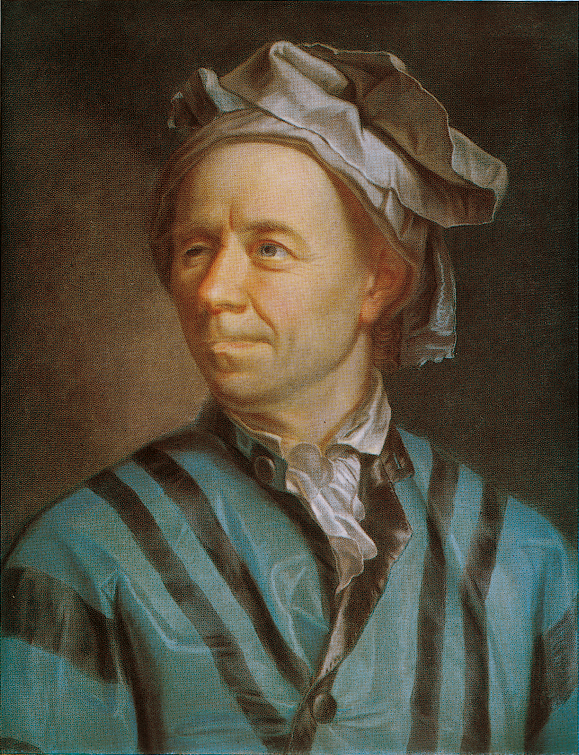
\includegraphics[width=1.5\paperwidth]{Euler.png}};    

\draw (8,-18) 
	node [fill=white!70, fill opacity=1,text opacity=1,inner sep=1cm]
	{\Huge\centering\bfseries\sffamily\parbox[c][][t]{\paperwidth}{\centering
	 Teoria dos Números 1\\[15pt] % Book title
	{\Large Notas de aula transcritas por Caio Tomás de Paula} \\[20pt] % Subtitle
	{\huge Prof. Dr. Hemar Teixeira Godinho}}}; % Author name
\end{tikzpicture}

\pagestyle{fancy} \addtolength{\headwidth}{\marginparsep}
\addtolength{\headwidth}{-0.3cm}
\renewcommand{\headrulewidth}{1pt}

\fancyhf{} \fancyhead[RO,RE]{\small\bfseries\textrm \thepage}
\fancyhead[LO]{\small\bfseries\textrm \leftmark}
\fancyhead[LE]{\small\bfseries\textrm \rightmark}

\newpage

\pagenumbering{roman}
\tableofcontents
\newpage
\pagenumbering{arabic}

\setlength{\baselineskip}{7mm}

\section{Introdução}
\hspace{12pt} Esse documento é uma coletânea, em PDF, das notas de aulas ministradas pelo professor Hemar Godinho (UnB), durante o curso de Teoria dos Números 1, ministrado no semestre letivo de 2020/1.

\section{Divisibilidade e o Algoritmo de Euclides}
\hspace{12pt} No decorrer desse documento, denotaremos:
\begin{itemize}
	\item os números naturais por $\mathbb{N} = \left\{ 1, 2, \dots \right\}$;
	\item os números inteiros por $\mathbb{Z} = \left\{\dots, -2, -1, 0, 1, 2, \dots \right\}$;
	\item os números racionais por $\mathbb{Q} = \left\{ \displaystyle{\frac{a}{b}\ \Big| \ a,b\in\mathbb{Z}}, b\neq 0 \right\}$;
	\item os números primos por $\mathbb{P}$.
\end{itemize}
\begin{definition}
	Sejam $a,b\in\mathbb{Z}$. Dizemos que $a$ {\em divide} $b$ se existe $c\in\mathbb{Z}$ tal que $b = ac$ e escrevemos $a|b$. Do contrário, $a\nmid b$ ($a$ não divide $b$).
\end{definition}
\begin{example}
	$5|10$, pois $10 = 5\cdot 2$, mas $3\nmid 10$, pois $\nexists c\in\mathbb{Z}$ tal que $10 = 3c$. 
\end{example}
\begin{definition}
	Se $a|b$, dizemos que $b$ é um {\em múltiplo} de $a$.
\end{definition}
\begin{lemma}
	\label{lema 1}
	Sejam $a,b,c\in\mathbb{Z}$. Se $a|b$ e $b|c$, então $a|c$.
\end{lemma}
\begin{proof}
	Se $a|b$, então $b = ak_1, k_1\in\mathbb{Z}$. Além disso, se $b|c$, então $c = bk_2, k_2\in\mathbb{Z}$. Portanto, $c = a(k_1k_2) = ak_3, \ k_3=k_1k_2\in\mathbb{Z}$. Logo, $a|c$.
\end{proof}
\begin{lemma}
	\label{lema 2}
	Sejam $a,b,c\in\mathbb{Z}$. Se $a|b$ e $a|c$, então $a|\lambda b + \mu c$, para quaisquer $\lambda, \mu\in\mathbb{Z}$.
\end{lemma}
\begin{proof}
	Por hipótese, sabemos que $b = ak_1$ e $c = ak_2$. Daí, quaisquer que sejam $\lambda,\mu\in\mathbb{Z}$, sabemos que $\lambda b + \mu c = \lambda ak_1 + \mu ak_2 = a(\lambda k_1 + \mu k_2) = ak_3$. Logo, $a|\lambda b + \mu c$.
\end{proof}
\begin{example}
	$5|10$ e $5|15 \Rightarrow 5|2\cdot 10 - 15$. 
\end{example}
\par\textbf{Princípio da Boa Ordenação (PBO):} todo conjunto de inteiros limitado inferiormente tem um menor elemento.
\begin{theorem}[Teorema de Euclides]
	\label{euclides}
	Sejam $a,b\in\mathbb{N}$ quaisquer. Então, existe um único par $q,r\in\mathbb{Z}$ tal que 
	\begin{align*}
	a = bq + r, \hspace{0.6cm} 0\leq r < b
	\end{align*}
\end{theorem}
\begin{proof}
	(Existência) Se $a<b$, tome $q = 0$ e $r = a<b$. Se $a = b$, tome $q = 1$ e $r = 0$.
	
	Suponha, então, $a > b$ e considere
	\begin{align*}
	M = \left\{ a - bx \ | \ x\in\mathbb{Z} \right\}.
	\end{align*}
	Observe que 
	\begin{align*}
	M = \left\{ \dots, a - 2b, a-b, a, a+b, a+2b, \dots \right\}.
	\end{align*}
	Seja 
	\begin{align*}
	M_+ = \left\{ m\in M \ | \ m\geq 0 \right\}\subseteq\mathbb{N}\cup\left\{0\right\}
	\end{align*}
	Pelo PBO, existe $r\in M_+$ tal que $r\leq m, \forall m\in M_+$. Como $r\in M_+\subset M$, existe $q\in\mathbb{Z}$ tal que $a - bq = r$, ou seja, $a = bq + r, r\geq 0$. Falta mostrar que $r < b$. Suponha $r\geq b$. Então, $r - b\geq 0$, i.e., $a - b(q+1) \geq 0$. Logo, $r^\ast = r-b\in M_+$ e $r^\ast < r$, o que é absurdo pois $r$ é o menor elemento de $M_+$. Portanto, $0\leq r < b$.
	
	(Unicidade) Suponha que $a = bq^\ast + r^\ast, \text{ com } q^\ast,r^\ast\in\mathbb{Z}$ e $0\leq r^\ast < b$. Se $r = r^\ast$, temos 
	\begin{align*}
	a = bq + r = bq^\ast + r^\ast \Rightarrow b(q - q^\ast) = r - r^\ast = 0 \Rightarrow q = q^\ast
	\end{align*}
	Suponha $r\neq r^\ast$ e, sem perda de generalidade, tome $r<r^\ast$. Temos $0\leq r < r^\ast < b$. Segue que $0\leq r^\ast - r < b$ e, como $b(q - q^\ast) = r^\ast - r$, temos $0\leq b(q - q^\ast) < b$. Mas $b\in\mathbb{N}$ e $q - q^\ast\in\mathbb{Z}_+$. Logo, temos que é absurdo pois $r < r^\ast$. 
	
	Portanto, $q,r\in\mathbb{Z}$ são únicos.
\end{proof}
\section{Máximo Divisor Comum (MDC)}
\hspace{12pt} \begin{definition}
	Sejam $a,b\in\mathbb{Z}$. Dizemos que $d\in\mathbb{N}$ é o {\em máximo divisor comum} entre $a$ e $b$ se:
	\begin{enumerate}
		\item $d|a$ e $d|b$
		\item se $d^\ast |a$ e $d^\ast |b$, então $d^\ast\leq d$
	\end{enumerate}
Denotamos $d = \mdc(a,b)$.
\end{definition}
\begin{example}
	Vamos calcular o $\mdc(18,14)$. Os divisores positivos de $18$ e $14$ são:
	\begin{align*}
	18: 1, 2, 3, 6, 9, 18 \\
	14: 1, 2, 7, 14
	\end{align*}
	Logo, $\mdc(18,14) = 2$.
\end{example}
\begin{lemma}
	\label{lema 3}
	Sejam $a,b\in\mathbb{Z}^\ast$, e seja $d = \mdc(a,b)$. Então, 
	\begin{align*}
	\mdc\left( \frac{a}{d}, \frac{b}{d} \right) = 1
	\end{align*}
\end{lemma}
\begin{proof}
	Como $d|a$ e $d|b$, temos $\displaystyle{ \frac{a}{d}, \frac{b}{d}\in\mathbb{Z}^\ast }$. Seja $\displaystyle{d^\ast = \mdc\left( \frac{a}{d}, \frac{b}{d} \right)}$. Logo, $\displaystyle{\frac{a}{d} = \lambda_1d^\ast}$ e $\displaystyle{\frac{b}{d} = \lambda_2d^\ast}$, ou seja, $a = \lambda_1dd^\ast$ e $b = \lambda_2dd^\ast$, $\lambda_1, \lambda_2\in\mathbb{Z}$. Portanto, $dd^\ast |a$ e $dd^\ast |b$. Como $d = \mdc(a,b)$ e $d^\ast\in\mathbb{N}$, segue que $dd^\ast\leq d \Rightarrow d^\ast = 1$.
\end{proof}
\begin{definition}
	Se $\mdc(a,b) = 1$, dizemos que $a$ e $b$ são {\em coprimos} ou {\em primos entre si}.
\end{definition}
\begin{remark}
	\label{obs 1}
	Sejam $a,b\in\mathbb{Z}^\ast$. Note que $\mdc(a,b) = \mdc(-a,b) = \mdc(a,-b) = \mdc(-a,-b)$.
\end{remark}
\begin{lemma}
	\label{lema 4}
	Sejam $a,b\in\mathbb{Z}^\ast$ e $d = \mdc(a,b)$. Então, existem inteiros $r,s$ tais que $d = ra + sb$.
\end{lemma}
\begin{proof}
	Pela Observação \eqref{obs 1}, podemos tomar $a,b\in\mathbb{N}$. Seja 
	\begin{align*}
	M = \left\{ ax + by \ | \ x,y\in\mathbb{Z} \right\} = \left\{ \dots, -2a - 2b, -2a - b, -a-2b, -a-b, -a, -b, 0, a, b, \dots \right\}.
	\end{align*}
	Seja \begin{align*}
	P = \left\{ m\in M \ | \ m\geq 1 \right\}\subseteq\mathbb{N}
	\end{align*}.
	Pelo PBO, $P$ tem um menor elemento $d^\ast$ e, como $P\subset M$, segue que $d^\ast = ra + sb$ para algum par $r,s\in\mathbb{Z}$. Vamos mostrar que $d^\ast |a$ e $d^\ast |b$. Pelo Algoritmo de Euclides, segue que $a = d^\ast q + r, 0\leq r < d^\ast$. Daí, $r = a - d^\ast q = a - q(ra + sb) = a(1 - qr) + b(-qs)$, ou seja, $r\in M$ e $r\geq 0$. Se $r = 0$, $d^\ast |a$. Se $r\geq 1$, então $r\in P$ e $r<d^\ast$, o que é absurdo pois $d^\ast$ é o menor elemento de $P$. Portanto, $r=0$ e $d^\ast |a$. 
	
	Também pelo Algoritmo de Euclides, temos $b = q_0d^\ast + r_0, 0\leq r_0 < d^\ast$. Analogamente ao que foi feito acima, concluímos que $d^\ast |b$. Falta mostrar que $d^\ast = d$. Como $d^\ast |a$ e $d^\ast |b$, temos, por definição, $d^\ast\leq d$. Por outro lado, como $d|a$ e $d|b$, segue do Lema \eqref{lema 2} que $d|ra+sb = d^\ast$, ou seja, $d\leq d^\ast$. Como $d,d^\ast\in\mathbb{N}$, segue que $d = d^\ast$. 
\end{proof}
\par Vale observar que, além de demonstrar que $\mdc(a,b)$ pode ser escrito como combinação linear de $a$ e $b$, mostramos que o $\mdc$ é, na verdade, a {\em menor} dessas combinações.
\begin{corollary}
	Seja $d = \mdc(a,b)$. Se $d_0|a$ e $d_0|b$, então $d_0|d$.
\end{corollary}
\begin{proof}
	Pelo Lema \eqref{lema 4}, $\exists r,s\in\mathbb{Z}$ tais que $d = ra + sb$. Como $d_0|a$ e $d_0|b$, segue do Lema \eqref{lema 2} que $d_0|ra + sb$, i.e., $d_0|d$.
\end{proof}
\begin{lemma}
	\label{lema 5}
	Se $a|bc$ e $\mdc(a,b) = 1$, então $a|c$.
\end{lemma}
\begin{proof}
	Sabemos que existem $r,s\in\mathbb{Z}$ tais que $1 = ra+sb$ (Lema \eqref{lema 4}). Também sabemos que $bc = at, t\in\mathbb{Z}$. Daí, 
	\begin{align*}
	c = c\cdot 1 = c(ra + sb) = acr + bcs = acr + ast = (cr + st)a \hspace{0.2cm} \therefore \hspace{0.2cm}a|c
	\end{align*}
\end{proof}
\begin{lemma}
	\label{lema 6}
	Sejam $a,b\in\mathbb{N}$ e tome $a = bq+r, 0\leq r < b$. Então, $\mdc(a,b) = \mdc(b,r)$.
\end{lemma}
\begin{proof}
	Sejam $d = \mdc(a,b)$ e $d^\ast = \mdc(b,r)$. Pelo Lema \eqref{lema 2}, segue que $d|r$, pois $r = a - bq$ e $d|a$ e $d|b$. Logo, como $d|b$ e $d|r$, segue do Corolário que $d|d^\ast$.
	
	Por outro lado, sabemos que $d^\ast |b$ e $d^\ast |r$. Pelo Lema \eqref{lema 2}, $d^\ast |bq+r=a$ e, pelo Corolário, $d^\ast |d$. Como $d,d^\ast\in\mathbb{N}$, segue que $d = d^\ast$.
\end{proof}
\section{Algoritmo de Euclides para o MDC}
\hspace{12pt} Sejam $a,b\in\mathbb{N}$. Pelo Algoritmo de Euclides, temos
\begin{align*}
a &= bq + r, \hspace{0.8cm} 0\leq r < b \\
b &= rq_1 + r_1, \hspace{0.45cm} 0\leq r_1 < r < b \\
r &= r_1q_2 + r_2, \hspace{0.3cm} 0\leq r_2 < r_1 < r < b \\
r_1 &= r_2q_3 + r_3, \hspace{0.3cm} 0\leq r_3 < r_2 < r_1 < r < b \\
&\hspace{0.15cm}\vdots 
\end{align*}
\par Como há $b$ inteiros entre $0$ e $b$, esse algoritmo tem, no máximo, $b$ passos, i.e., para algum $n>b$ teremos
\begin{align*}
&\hspace{0.15cm}\vdots \\
r_{n-3} &= r_{n-2}q_{n-1} + r_{n-1}, \hspace{0.3cm} 0 < r_{n-1} < r_{n-2} < \cdots < b \\
r_{n-2} &= r_{n-1}q_n + r_n, \hspace{0.3cm} r_n = 0
\end{align*}
\par Logo, $r_{n-1}|r_{n-2}$, ou seja, $\mdc(r_{n-1}, r_{n-2}) = r_{n-1}$, pois $r_{n-1} < r_{n-2}$. Pelo Lema \eqref{lema 6}, segue que
\begin{align*}
\mdc(a,b) = \mdc(b,r) = \mdc(r,r_1) = \cdots = \mdc(r_{n-2}, r_{n-1}) = r_{n-1},
\end{align*}
ou seja, $\mdc(a,b) = r_{n-1}$.
\begin{example}
	Calcule $\mdc(153, 27)$. Temos
	\begin{align*}
	153 &= 27\cdot 5 + 18 \\
	27 &= 18\cdot 1 + 9 \\
	18 &= 9\cdot 2,  
	\end{align*}
	logo $\mdc(153, 27) = 9$.
\end{example}
\begin{example}
	Calcule $\mdc(190, 136)$ e determine $r,s\in\mathbb{Z}$ tais que $\mdc(190,136) = 190r + 136s$. Temos
	\begin{align*}
	190 &= 136\cdot 1 + 54 \\
	136 &= 54\cdot 2 + 28 \\
	54 &= 28\cdot 1 + 26 \\
	28 &= 26\cdot 1 + 2 \\
	26 &= 2\cdot 13, 
	\end{align*}
	logo $\mdc(190, 136) = 2$. Reescrevendo os restos, temos
	\begin{align*}
	54 &= 190 - 136 \\
	28 &= 136 - 2\cdot 54 = 136 - 2(190 - 136) = 3\cdot 136 - 2\cdot 190 \\
	26 &= 54 - 28 = (190 - 136) - (3\cdot 136 - 2\cdot 190) = -4\cdot 136 + 3\cdot 190 \\
	2 &= 28 - 26 = (3\cdot 136 - 2\cdot 190) - (-4\cdot 136 + 3\cdot 190) = 190\cdot(-5) + 136\cdot(7)
	\end{align*}
\end{example}
\section{Equação diofantina linear em duas variáveis}
\hspace{12pt} Sejam $a,b,c\in\mathbb{Z}$ e considere a equação
\begin{align*}
ax + by = c.
\end{align*}
\par Queremos determinar todas as soluções inteiras dessa equação.
\begin{lemma}
	\label{lema 7}
	A equação $ax + by = c$ tem solução inteira se, e somente se, $\mdc(a,b)|c$. 
\end{lemma}
\begin{proof}
	Suponha que $x_0, y_0\in\mathbb{Z}$ é solução de $ax + by = c$, ou seja, $ax_0 + by_0 = c$. Seja $d = \mdc(a,b)$. Então, como $d|a$ e $d|b$, pelo Lema \eqref{lema 2}, $d|c$. Reciprocamente, suponha que $d|c$. Então, $c = \lambda d, \lambda\in\mathbb{Z}$. Pelo Lema \eqref{lema 4}, existem $r,s\in\mathbb{Z}$ tais que $d = ar + bs$, logo $c = \lambda d = a(\lambda r) + b(\lambda s)$, ou seja, tomando $x_0 = \lambda r$ e $y_0 = \lambda s$ temos que $x_0, y_0$ é solução de $ax + by = c$.
\end{proof}
\begin{lemma}
	\label{lema 8}
	Suponha que $x_0,y_0\in\mathbb{Z}$ seja solução de $ax + by = c$. Então
	\begin{align*}
	x_t = x_0 + \frac{b}{d}t \hspace{0.3cm} \text{ e } \hspace{0.3cm} y_t = y_0 - \frac{a}{d}t, \hspace{0.3cm} d = \mdc(a,b)
	\end{align*}
	é também solução de $ax + by = c, \forall t\in\mathbb{Z}$. Além disso, todas as soluções de $ax + by = c$ são obtidas dessa forma (i.e., se $x^\ast, y^\ast\in\mathbb{Z}$ é solução de $ax + by = c$, então existe $t\in\mathbb{Z}$ tal que $x^\ast = x_t$ e $y^\ast = y_t$).
\end{lemma}
\begin{proof}
	Primeiro, vamos mostrar que $\forall t\in\mathbb{Z}$, $x_t, y_t$ é solução de $ax + by = c$. Note que 
	\begin{align*}
	ax_t + by_t &= ax_0 + by_0 + \frac{ab}{d}t - \frac{ba}{d}t \\
	&= ax_0 + by_0 \\
	&= c.
	\end{align*}
	Portanto, $x_y, y_t$ é solução.
	
	Suponha, agora, que $x^\ast, y^\ast$ é solução de $ax + by = c$. Então, 
	\begin{align*}
	ax^\ast + by^\ast = c = ax_0 + by_0 \Rightarrow a(x^\ast - x_0) = b(y_0 - y^\ast).
	\end{align*}
	Como $d|a$ e $d|b$, segue que 
	\begin{align*}
	\frac{a}{d}(x^\ast - x_0) = \frac{b}{d}(y_0 - y^\ast).
	\end{align*}
	Pelos Lemas \eqref{lema 3} e \eqref{lema 5}, temos
	\begin{align*}
	\frac{a}{d}\Big| (y_0 - y^\ast) \hspace{0.3cm} \text{ e } \frac{b}{d}\Big| (x^\ast - x_0), \hspace{0.3cm} \text{ pois } \mdc\left( \frac{a}{d}, \frac{b}{d} \right) = 1 \\
	\Rightarrow y_0 - y^\ast = t\frac{a}{d} \hspace{0.3cm} \text{ e } x^\ast - x_0 = k\frac{b}{d}, \hspace{0.2cm} t,k\in\mathbb{Z}.
	\end{align*}
	Agora, 
	\begin{align*}
	c &= ax^\ast + by^\ast = a\left( x_0 + \frac{b}{d}k \right) + b\left( y_0 - \frac{a}{d}t \right) \\
	\Leftrightarrow c &= ax^\ast + by^\ast = ax_0 + by_0 + \frac{ab}{d}(k-t) \\
	\Leftrightarrow c &= c + \frac{ab}{d}(k-t) \\
	\Leftrightarrow &\frac{ab}{d}(k-t) = 0 \underset{a,b\in\mathbb{N}}{\Rightarrow} k = t.
	\end{align*}
	Portanto, $x^\ast = x_0 + \displaystyle{ \frac{b}{d}t }$ e $y^\ast = y_0 - \displaystyle{ \frac{a}{d}t }$.
\end{proof}
\begin{corollary}
	Sejam $a,b\in\mathbb{Z}$. Se $\mdc(a,b) = 1$, então $ax + by = c$ tem infinitas soluções inteiras, independentemente do valor de $c$.
\end{corollary}
\begin{proof}
	Do Lema \eqref{lema 7}, segue que essa equação sempre tem solução pois $\mdc(a,b) = 1$ e $1|c$, para todo $c\in\mathbb{Z}$. Pelo Lema \eqref{lema 8}, segue que há infinitas soluções.
\end{proof}
\begin{example}
	Encontre todas as soluções de $3x + 5y = 14$.
	
	Como $\mdc(3,5) = 1$ e $1|14$, existem infinitas soluções. Note que $1 = 3\cdot 2 - 1\cdot 5$, logo $14 = 3(2\cdot 14) + 5(-1\cdot 14)$. Portanto, $(x_0, y_0) = (28,-14)$ é solução, e as demais são
	\begin{align*}
	\begin{cases}
	x_t = 28 + 5t \\
	y_t = -14 - 3t
	\end{cases}, t\in\mathbb{Z}.
	\end{align*}
\end{example}
\begin{remark}
	\label{obs 2}
	O exemplo acima ilustra que basta conhecer $r,s\in\mathbb{Z}$ tais que $\mdc(a,b) = ra + sb$ para encontrar uma solução para $ax + by = c$. Se $d = \mdc(a,b)$ e $d|c$, escreva $c = \lambda d = \lambda(ra + sb) = a(\lambda r) + b(\lambda s)$, ou seja,
	\begin{equation*}
	x_0 = \lambda r \hspace{0.3cm} \text{ e } y_0 = \lambda s
	\end{equation*}
	é solução. É possível obter, do Algoritmo de Euclides para o cálculo do MDC, os valores de $r$ e $s$. Observe o exemplo a seguir.
\end{remark}
\begin{example}
	Encontre todas as soluções de
	\begin{equation*}
	190x + 136y = 14
	\end{equation*}
	Num exemplo anterior, descobrimos que $\mdc(190,136) = 2$. Como $2|14$, há infinitas soluções. Também vimos que
	\begin{align*}
	2 = 190\cdot(-5) + 136\cdot 7,
	\end{align*}
	logo 
	\begin{align*}
	14 = 190\cdot(-35) + 136\cdot(49),
	\end{align*}
	e temos 
	\begin{align*}
	x_0 = -35, \hspace{0.2cm} y_0 = 49.
	\end{align*}
	Portanto, as soluções são
	\begin{align*}
	\begin{cases}
	x_t = -35 + 68t \\
	y_t = 49 - 95t
	\end{cases},t\in\mathbb{Z}.
	\end{align*}
\end{example}
\section{Indução Matemática}
\hspace{12pt} Seja $p(n)$ uma proposição lógica que dependa de $n\in\mathcal{N}\subseteq\mathbb{N}\cup\left\{0\right\}$.
\begin{example}
	$p(n) = $ ``A soma dos primeiros $n$ números naturais consecutivos é igual a $\displaystyle{\frac{n(n+1)}{2}}$''.
	
	Em linguagem matemática, 
	\begin{align*}
	p(n) = ``1 + 2 + \cdots + n = \frac{n(n+1)}{2}"
	\end{align*}
	Essa é uma proposição lógica que depende de $n$.
\end{example}
\begin{theorem}[Indução Matemática]
	Seja $\mathcal{N}\subseteq\mathbb{N}\cup\left\{0\right\}$ e escreva $\mathcal{N} = \left\{n_0, n_1, \dots \right\}$ com $n_0 < n_1 < \dots$.
	
	Seja $p(n)$ uma proposição lógica que dependa de $n\in\mathbb{N}$. Se
	\begin{align*}
	\begin{cases}
	p(n_0) \text{ é verdadeira} \\
	p(n_k) \Longrightarrow p(n_{k+1}) \forall n_k\in\mathcal{N}
	\end{cases}
	\end{align*}
	então $p(n)$ é verdadeira $\forall n\in\mathcal{N}$.
\end{theorem}
\begin{proof}
	Seja $\mathcal{F} = \left\{ n\in\mathcal{N} \ | \ p(n) \text{ é falsa} \right\}$. Queremos mostrar que, sob as hipóteses do teorema, $\mathcal{F} = \emptyset$, i.e., $p(n)$ é verdadeira $\forall n\in\mathcal{N}$. Como $\mathcal{F}\subset\mathcal{N}\subseteq\mathbb{N}\cup\left\{0\right\}$, pelo PBO existe $n_r\in\mathcal{F}$ tal que $n_r\leq m, \forall m\in\mathcal{F}$. 
	
	Pela primeira hipótese do teorema, $n_r > n_0$ (pois $p(n)$ é verdadeira) e, portanto, $p(n_0), \dots, p(n_{r-1})$ são verdadeiras.
	
	Pela segunda hipótese, temos $p(n_r)$ verdadeira, o que é absurdo pois $n_r\in\mathcal{F}$. Logo, $\mathcal{F} = \emptyset.$ 
\end{proof}
\begin{example}
	Mostre que, $\forall n\in\mathbb{N}$, $1 + 2 + \cdots + n = \displaystyle{\frac{n(n+1)}{2}}$. 
	
	Vamos aplicar indução. Primeiro, note que para $n=1$, temos $1 = 1$ e $p(1)$ é verdadeira. Suponha que, para $m\in\mathbb{N}$, $p(m)$ é verdadeira, ou seja
	\begin{align*}
	1 + 2 + \cdots + m = \frac{m(m+1)}{2}.
	\end{align*}
	Daí, segue que
	\begin{align*}
	1 + 2 + \cdots + m + m+1 &= \frac{m(m+1)}{2} + m+1 \\
	&= \frac{(m+1)(m+2)}{2}
	\end{align*}
	e $p(m+1)$ é verdadeira. Logo, segue por indução que $p(n)$ é sempre verdadeira.
\end{example}
\begin{remark}
	No caso da indução matemática, chamamos a primeira hipótese do teorema de {\em caso particular} e a afirmação ``se $p(n_k)$ é verdadeira'' de {\em hipótese de indução}.
\end{remark}
\begin{example}
	Mostre que, $\forall n\in\mathbb{N}$, temos
	\begin{align*}
	1 + x + \cdots + x^n = \frac{x^{n+1} - 1}{x - 1}.
	\end{align*} 
	
	Para o caso particular $n=1$, temos $1 + x = \displaystyle{\frac{x^2 - 1}{x - 1} = x+1}$. 
	
	Suponha, por hipótese de indução, que 
	\begin{align*}
	1 + x + \cdots + x^k = \frac{x^{k+1} - 1}{x - 1}.
	\end{align*}
	Considere
	\begin{align*}
	1 + x + \cdots + x^k + x^{k+1} &= \frac{x^{k+1} - 1}{x - 1} + x^{k+1} \\
	&= \frac{ x^{k+1} - 1 + x^{k+2} - x^{k+1} }{x-1} \\
	&= \frac{x^{k+2} - 1}{x-1}.
	\end{align*}
	Logo, $p(k+1)$ também é verdadeira e, por indução, $p(n)$ é verdadeira para todo $n\in\mathbb{N}$.
\end{example}
\begin{example}
	Mostre que, $\forall n\in\mathbb{N}$, $n^3 + (n+1)^3 + (n+2)^3$ é sempre divisível por $9$.
	
	Para o caso particular $n=1$, temos $1^3 + 2^3 + 3^3 = 36$ e $9|36$.
	
	Suponha, por hipótese de indução, que $9|m^3 + (m+1)^3 + (m+2)^3$. Considere 
	\begin{align*}
	(m+1)^3 + (m+2)^3 + (m+3)^3 &= (m+1)^3 + (m+2)^3 + (m^3 + 9m^2 + 27m + 27) \\
	&= \big(m^3 + (m+1)^3 + (m+2)^3 \big) + 9m^2 + 27m + 27 \\
	&= 9M + 9(m^2+2m+3),
	\end{align*}
	que claramente é divisível por $9$. Logo, $p(n)$ é verdadeira para todo $n\in\mathbb{N}$.
\end{example}
\begin{example}
	Mostre que, $\forall n\in\mathbb{N}$, 
	\begin{align*}
	1^3 + 2^3 + \cdots + n^3 = (1 + 2 + \cdots + n)^2
	\end{align*}
	Para o caso particular $n=1$, temos $1^3 = 1^2$. Suponha, por hipótese de indução, que
	\begin{align*}
	1^3 + 2^3 + \cdots + k^3 = (1 + 2 + \cdots + k)^2
	\end{align*}
	e considere
	\begin{align*}
	1^3 + 2^3 + \cdots + k^3 + (k+1)^3 &= (1 + 2 + \cdots + k)^2 + (k+1)^3 \\
	&= \left( \frac{k(k+1)}{2} \right)^2 + (k+1)^3 \\
	&= \frac{ k^2(k+1)^2 + 4(k+1)^3 }{4} \\
	&= \frac{(k+1)^2(k^2 + 4k + 4)}{4} \\
	&= \left( \frac{(k+1)(k+2)}{2} \right)^2 \\
	&= (1 + 2 + \cdots + k + k+1)^2.
	\end{align*}
	Logo, segue por indução que a proposição vale $\forall n\in\mathbb{N}$. 
\end{example}
\section{Números primos}
\hspace{12pt} \begin{definition}
	Seja $p\in\mathbb{N}, p\neq 1$. O número $p$ é chamado de {\em primo} se os únicos divisores positivos de $p$ são $1$ e $p$.
\end{definition}
\begin{example}
	$2, 3, 5, 7, 11, 13, 17, 19, 23$ são primos.
\end{example}
\begin{lemma}
	\label{lema 9}
	Seja $p$ um primo e $a\in\mathbb{Z}$. Se $p\nmid a$, então $\mdc(a,p) = 1$.
\end{lemma}
\begin{proof}
	Seja $d = \mdc(a,p)$. Logo, $d|p$ e $d|a$. Como $p$ é primo, $d = 1$ ou $d = p$. Se $d=p$, então $p|a$, absurdo. Portanto, $d = 1$.
\end{proof}
\begin{lemma}
	\label{lema 10}
	Sejam $p$ primo e $a,b\in\mathbb{Z}$. Se $p|ab$, então $p|a$ ou $p|b$.
\end{lemma}
\begin{proof}
	Suponha que $p\nmid a$. Pelo Lema \eqref{lema 9}, $\mdc(a,p) = 1$. Como $p|ab$, pelo Lema \eqref{lema 5} temos que $p|b$.
\end{proof}
\begin{lemma}
	\label{lema 11}
	Sejam $p, q_1, q_2$ primos. Se $p|q_1q_2$, então ou $p = q_1$ ou $p=q_2$.
\end{lemma}
\begin{proof}
	Pelo Lema \eqref{lema 10}, $p|q_1$ ou $p|q_2$. Suponha, sem perda de generalidade, que $p|q_1$. Como $p$ é primo, $p\neq 1$ e, como $q_1$ é primo, devemos ter $p=q_1$.
\end{proof}
\begin{lemma}
	\label{lema 12}
	Sejam $p, q_1, \dots, q_r$ primos. Se $p|q_1q_2\cdots q_r$, então existe $j\in\left\{ 1, 2, \dots, r \right\}$ tal que $p = q_j$.
\end{lemma}
\begin{proof}
	Vamos proceder por indução em $r$. Como caso particular, temos $r=1$: se $p|q_1$, então $p=q_1$. Suponha, por hipótese de indução, que se $p|q_1q_2\cdots q_k$, então $p|q_j$ para algum $j\in\left\{1, 2, \dots, k \right\}$. Considere 
	\begin{align*}
	\underbrace{q_1\cdots q_k}_{a}\cdot \underbrace{q_{k+1}}_{b} = ab.
	\end{align*}
	Pelo Lema \eqref{lema 10}, sabemos que $p|a$ ou $p|b$, i.e., $p|q_1\cdots q_k$ ou $p|q_{k+1}$. Se $p|q_{k+1}$, então $p = q_{k+1}$, pois $p$ e $q_{k+1}$ são primos. Se $p|q_1\cdots q_k$, segue da hipótese de indução que $p|q_j$ para algum $j\in\left\{1, 2, \dots, k \right\}$.
	
	Logo, segue por indução que o lema é verdadeiro.
\end{proof}
\begin{definition}
	Seja $m\in\mathbb{N}, m\neq 1$. Se $m$ não é primo, $m$ é chamado de {\em composto}.
\end{definition}
\begin{lemma}
	\label{lema 13}
	Sejam $p,q$ primos distintos. Se $p|a$ e $q|a$, então $pq|a$.
\end{lemma}
\begin{proof}
	Como $p|a$, $a = pM, M\in\mathbb{Z}$. Como $q|a$, segue que $q|pM$. Pelo Lema \eqref{lema 10}, $q|p$ ou $q|M$. Se $q|p$, então $q=p$, absurdo. Portanto, $q|M$, i.e., $M = qR, R\in\mathbb{Z}$. Logo, $a = pqR$, ou seja, $pq|a$.
\end{proof}
\par O resultado principal dessa seção é o Teorema Fundamental da Aritmética, mas antes de apresentá-lo precisamos de uma outra versão do Teorema de Indução Matemática.
\begin{theorem}[Indução Matemática -- 2$^{\text{\underline{a}}}$ forma]
	Seja $\mathcal{N}\subseteq\mathbb{N}\cup\left\{0\right\}$ e escreva $\mathcal{N} = \left\{ n_0, n_1, n_2, \dots  \right\}$ com $n_0 < n_1 <n_2 < \cdots $. Seja $p(n)$ uma proposição lógica que dependa de $n\in\mathcal{N}$. Se
	\begin{align*}
	\begin{cases}
	p(n_0) \text{ é verdadeira } \\
	p(n_j) \text{ é verdadeira para todo } j<k \text{ então } p(n_k) \text{ é verdadeira}
	\end{cases}
	\end{align*}
	então $p(n)$ é verdadeira $\forall n\in\mathcal{N}$.
\end{theorem}
\begin{proof}
	A mesma do Teorema de Indução Matemática.
\end{proof}
\section{Fundamental da Aritmética}
\begin{theorem}[Teorema Fundamental da Aritmética]
	Todo número natural maior que $1$ pode ser escrito de maneira única (a menos de ordem) como um produto de primos.
\end{theorem}
\begin{proof}
	(Existência) Vamos proceder por indução sobre $n$. Para o caso particular $n=2$, podemos escrever $2=2$.
	
	Suponha, por hipótese de indução, que todo $r\in\mathbb{N}, 1 < r < m, m\in\mathbb{N}$, pode ser escrito como produto de primos. Se $m$ é primo, $m$ é produto de um primo.
	
	Suponha $m$ composto e $m = uv, 1 < u,v < m$. Pela hipótese de indução, temos
	\begin{align*}
	u = p_1p_2\cdots p_r \hspace{0.3cm} &\text{ e } \hspace{0.3cm} v = q_1q_2\cdots q_s, \text{ logo} \\
	m = uv &= p_1\cdots p_rq_1\cdots q_s
	\end{align*} 
	também é um produto de primos.
	
	(Unicidade) Seja $n\in\mathbb{N}, n>1$ e suponha que
	\begin{align*}
	n = p_1\cdots p_r = q_1\cdots q_s, r\leq s.
	\end{align*}
	Logo, $p_1|q_1\cdots q_s$, ou seja, $\exists j\in\left\{ 1, 2, \dots, s \right\}$ tal que $p_1 = q_j$, pelo Lema \eqref{lema 12}. Reordenando os índices dos $q_i$'s, assuma $p_1 = q_1$. Então,
	\begin{align*}
	p_1p_2\cdots p_r = p_1q_2\cdots q_s \Rightarrow p_2p_3\cdots p_r = q_2q_3\cdots q_s.
	\end{align*}
	Continuando esse processo, teremos, eventualmente,
	\begin{align*}
	p_r = q_rq_{r+1}\cdots q_s, \text{ pois }r\leq s.
	\end{align*}
	Como $p_r$ é primo, segue que $r=s$ e $p_r=q_r$.
\end{proof}
\begin{lemma}
	\label{lema 14}
	Sejam $p_1, \dots, p_r$ primos distintos. Se $p_1^m|p_1^{t_1}\cdots p_r^{t_r}$, com $m, t_1, \dots, t_r\in\mathbb{N}\cup\left\{0\right\}$, então $m\leq t_1$.
\end{lemma}
\begin{proof}
	Suponha $m>t_1$ e escreva $m = t_1 + s, s\geq 1$. Daí, por hipótese, 
	\begin{align*}
	\lambda p_1^m = p_1^{t_1}p_2^{t_2}\cdots p_r^{t_r} \Longrightarrow \lambda p_1^{t_1}p_1^s = p_1^{t_1}p_2^{t_2}\cdots p_r^{t_r} \Longrightarrow \lambda p_1^s = p_2^{t_2}\cdots p_r^{t_r}.
	\end{align*}
	Contudo, isso contraria o TFA, pois do lado direito temos um número escrito como produto de primos $p_2, p_3, \dots, p_r$ e, do lado esquerdo, escrito como outro produto de primos, com o fator $p_1^s$. Isso é absurdo, pois a fatoração é única, logo $m\leq t_1$. 
\end{proof}
\begin{lemma}
	\label{lema 15}
	Seja $n = p_1^{r_1}\cdots p_s^{r_s}$, com $p_1, p_2, \dots, p_r$ primos distintos. Então, $d|n$ se, e somente se, $d = p_1^{l_1}\cdots p_s^{l_s}$, com $0\leq l_i\leq r_i, i = 1, 2, \dots, s$.
\end{lemma}
\begin{proof}
	Se $d|n$, então $\lambda d = p_1^{r_1}\cdots p_s^{r_s}$. Seja $q$ primo tal que $q|d$. Como $d|n$, segue do Lema \eqref{lema 1} que $q|n$. Pelo Lema \eqref{lema 12}, temos $q\in\left\{p_1, \dots, p_s\right\}$. Assim, devemos ter 
	\begin{align*}
	d = p_1^{l_1}\cdots p_s^{l_s}.
	\end{align*}
	Agora, nem todos os primos podem estar na fatoração de $n$, e podemos ter $l_i = 0$ para algum $i$; por outro lado, o Lema \eqref{lema 14} nos diz que $l_i\leq r_i$. Desse modo, $0\leq l_i\leq r_i, \forall i$.
	
	Reciprocamente, suponha que $d = p_1^{l_1}\cdots p_s^{l_s}$, com $0\leq l_i\leq r_i, i = 1,2,\dots,s$. Como $l_i\leq r_i$, podemos escrever $r_i = l_i + k_i, k_i\in\mathbb{N}\cup\left\{0\right\}$. Daí, temos
	\begin{align*}
	n = p_1^{r_1}\cdots p_s^{r_s} &= \left( p_1^{l_1}\cdots p_s^{l_s} \right)\left( p_1^{k_1}\cdots p_s^{k_s} \right) \\
	&= d\lambda, \lambda\in\mathbb{Z}.
	\end{align*}
	Logo, $d|n$.
\end{proof}
\begin{lemma}
	\label{lema 16}
	Seja $a\in\mathbb{N}, a\geq 2$ e escreva $a = p_1^{r_1}\cdots p_s^{r_s}$ com $p_1, \dots, p_s$ primos distintos. O número de divisores positivos de $a$ é $\displaystyle{\prod_{i=1}^{s}(r_i+1)}$.
\end{lemma}
\begin{proof}
	O Lema \eqref{lema 15} nos diz que $d$ é um divisor positivo de $a$ se, e só se, $d = p_1^{l_1}\cdots p_s^{l_s}$, com $0\leq l_i\leq r_i$ e $i\leq s$. Portanto, para contar os divisores positivos de $a$ pode ser feita uma correspondência
	\begin{align*}
	p_1^{l_1}\cdots p_s^{l_s} \leftrightarrow (l_1, \dots, l_s),
	\end{align*}
	ou seja, contar a quantidade de $s$-uplas. Como $0\leq l_i\leq r_i$, o total é $\displaystyle{ \prod_{i=1}^{s}(r_i + 1) }$.
\end{proof}
\begin{example}
	Seja $a = 2\cdot 3\cdot 5^2$. Logo, o número de divisores positivos de $a$ é $(1+1)(1+1)(2+1) = 12$. A saber: $2^0\cdot 3^0\cdot 5^0, 2^1\cdot 3^0\cdot 5^0, 2^0\cdot 3^1\cdot 5^0, 2^0\cdot 3^0\cdot 5^1, 2^1\cdot 3^1\cdot 5^0, 2^1\cdot 3^0\cdot 5^1, 2^0\cdot 3^1\cdot 5^1, 2^0\cdot 3^0\cdot 5^2, 2^1\cdot 3^0\cdot 5^2, 2^0\cdot 3^1\cdot 5^2, 2^1\cdot 3^1\cdot 5^2, 2^1\cdot 3^1\cdot 5^1$.
\end{example}
\section{Mínimo Múltiplo Comum (MMC)}
\begin{definition}
	Sejam $a,b\in\mathbb{Z}$ e seja $m\in\mathbb{N}$. Dizemos que $m$ é o {\em mínimo múltiplo comum} de $a$ e $b$ se
	\begin{enumerate}
		\item $a|m$ e $b|m$
		\item se $a|m^\ast$ e $b|m^\ast$, então $m\leq m^\ast$
	\end{enumerate}
	Denotamos $m = \mmc(a,b)$.
\end{definition}
\begin{example}
	Determine $\mmc(12,20)$. Note que os múltiplos positivos são
	\begin{align*}
	&12: 12, 24, 36, 48, 60, 72, 84, \dots \\
	&20: 20, 40, 60, 80, \dots
	\end{align*}
	logo $\mmc(12,20) = 60$.
\end{example}
\begin{lemma}
	\label{lema 17}
	Sejam $a,b\in\mathbb{Z}$ e escreva $a = p_1^{r_1}\cdots p_s^{r_s}$ e $b = p_1^{l_1}\cdots p_s^{l_s}$, com $r_j,l_j\geq 0$ para $j = 1,2,\dots,s$ e $p_1 < p_2 < \cdots < p_s$ primos. Defina, para $1\leq j\leq s$, $v_j = \min\left\{ r_j, l_j \right\}$ e $u_j = \max\left\{ r_j,l_j \right\}$, e escreva $d = p_1^{v_1}\cdots p_s^{v_s}$, $m = p_1^{u_1}\cdots p_s^{u_s}$ . Então, $d = \mdc(a,b)$ e $m = \mmc(a,b)$.
\end{lemma}
\begin{proof}
	Pelo Lema \eqref{lema 15}, sabemos que $d|a$ e $d|b$, e se $d^\ast |a$ e $d^\ast |b$ então $d^\ast = p_1^{t_1}\cdots p_s^{t_s}$ com $t_j\leq r_j$ e $t_j\leq l_j$, logo $t_j\leq\min\left\{ r_j,t_j \right\}$, ou seja, $d^\ast|d$. Logo, $d = \mdc(a,b)$.
	
	Também do Lema \eqref{lema 15}, $a|m$ e $b|m$. Seja $m^\ast$ um múltiplo comum de $a$ e $b$, i.e., $a|m^\ast$ e $b|m^\ast$. Assim, 
	\begin{align*}
	m^\ast = a\lambda = p_1^{r_1}\cdots p_s^{r_s}\cdot\lambda \hspace{0.3cm}\text{ e }\hspace{0.3cm} m^\ast = b\delta = p_1^{l_1}\cdots p_s^{l_s}\cdot\delta .
	\end{align*}
	Em particular, $p_j^{u_j}|m^\ast$ com $j = 1,2,\dots,s$, logo $m|m^\ast$. Portanto, $m = \mmc(a,b)$.
\end{proof}
\begin{corollary}
	Seja $m = \mmc(a,b)$. Se $a|m^\ast$ e $b|m^\ast$, então $m|m^\ast$.
\end{corollary}
\begin{proof}
	Segue da demonstração do Lema \eqref{lema 17}.
\end{proof}
\begin{example}
	Sejam $a = 200 = 2^3\cdot 5^2$ e $b = 945 = 3^3\cdot 5\cdot 7$. Pelo Lema \eqref{lema 17}, $\mdc(a,b) = 2^0\cdot 3^0\cdot 5\cdot 7^0 = 5$ e $\mmc(a,b) = 2^3\cdot 3^3\cdot 5^2\cdot 7 = 37800$.
\end{example}
\begin{lemma}
	\label{lema 18}
	Sejam $a,b\in\mathbb{N}$. Então $\mdc(a,b)\cdot\mmc(a,b) = ab$.
\end{lemma}
\begin{proof}
	Escreva $a = \displaystyle{ \prod_{i=1}^{s}p_i^{r_i} }$ e $b = \displaystyle{ \prod_{i=1}^{s}p_i^{l_i} }$, com $p_1 < p_2 < \cdots < p_s$ primos. Pelo Lema \eqref{lema 17}, temos $\mdc(a,b) = \displaystyle{ \prod_{i=1}^{s}p_i^{ \min\left\{r_i,l_i\right\} } }$ e $\mmc(a,b) = \displaystyle{ \prod_{i=1}^{s}p_i^{ \max\left\{r_i,l_i\right\} } }$. Observe que $\min\left\{r_i,l_i\right\} + \max\left\{r_i,l_i\right\} = r_i+l_i$. Logo, $\mdc(a,b)\cdot\mmc(a,b) = \displaystyle{ \prod_{i=1}^{s}p_i^{l_i+r_i} } = ab$.
\end{proof}
\begin{theorem}
	O conjunto $\mathbb{P}$ dos números primos é infinito.
\end{theorem}
\begin{proof}
	Suponha $\mathbb{P}$ finito e escreva
	\begin{align*}
	\mathbb{P} = \left\{ p_1, p_2, \dots, p_k \right\}.
	\end{align*}
	Seja $m = p_1p_2\cdots p_k + 1$, logo $m\in\mathbb{N}$. Pelo TFA, temos
	\begin{align*}
	m = q_1q_2\cdots q_s, q_i\in\mathbb{P} \text{ para }i=1,2,\dots,s.
	\end{align*}
	Após renumeração de índices, assuma $q_1 = p_1$. Logo,
	\begin{align*}
	m = p_1q_2\cdots q_s = p_1p_2\cdots p_k + 1 \Rightarrow p_1q_2\cdots q_s - p_1p_2\cdots p_s = 1 \Rightarrow p_1\left( q_2\cdots q_s - p_2\cdots p_k \right) = 1 \Rightarrow p_1|1,
	\end{align*}
	o que é absurdo pois $p_1$ é primo. Portanto, $\mathbb{P}$ é infinito.
\end{proof}
\begin{remark}
	\label{obs 4}
	Seja $k\in\mathbb{N}, k\geq 2$. Como $k! = 1\cdot 2\cdots (k-1)\cdot k$, temos que $n|k!$ para todo $1\leq n\leq k$. Observe que a lista abaixo
	\begin{align*}
	k!+1, k!+2, \dots, k!+k
	\end{align*}
	é uma lista de $k$ naturais consecutivos e, como $k!+j$ é divisível por $j$ se $2\leq j\leq k$ e $k!+j > j$, compostos. Logo, sempre podemos encontrar intervalos de $\mathbb{N}$, arbitrariamente grandes, que não contêm primos.
\end{remark}
\begin{lemma}
	\label{lema 19}
	Todo $n\in\mathbb{N}$ composto tem um fator primo menor ou igual a $\sqrt{n}$.
\end{lemma}
\begin{proof}
	Como $n$ é composto, $n=p_1\cdots p_r$ com $p_1\leq \cdots \leq p_r$ primos e $r\geq 2$. Nesse caso, temos
	\begin{align*}
	n = p_1\left( p_2\cdots p_r \right)\geq p_1^2 \text{ pois } p_1\leq \cdots \leq p_r,
	\end{align*}
	logo $\sqrt{n}\geq p_1$, como queríamos.
\end{proof}
Há resultados muito bonitos sobre primos, cujas demonstrações estão além desse curso. Contudo, vale mencioná-los.
\begin{itemize}
	\item Euler (1737): seja $\mathbb{P}$ o conjunto dos primos. Então, $\displaystyle{\sum_{p\in\mathbb{P}} \frac{1}{p} }$ diverge;
	\item Dirichlet (1837): sejam $a,b\in\mathbb{N}$ com $\mdc(a,b) = 1$. Existem infinitos números primos da forma $an + b$, i.e., há infinitos primos na P.A.
	\begin{align*}
	a+b, 2a+b, 3a+b, \dots 
	\end{align*}
	\item Teorema dos Números Primos (Hadamard -- de la Vallée Poussin --- 1896): seja $x\in\mathbb{R}, x>1$ qualquer e defina $\pi(x)$ como a quantidade de primos menores que $x$. Daí,
	\begin{align*}
	\displaystyle{ \lim_{x\to\infty}{ \frac{\pi(x)}{x/\ln(x)} } = 1 }
	\end{align*}
\end{itemize}
\begin{remark}
	\label{obs 5}
	Embora o Teorema de Dirichlet seja difícil de demonstrar, vamos, a seguir, apresentar um caso onde conseguimos provar que existem infinitos primos nessa P.A.
\end{remark}
Pelo Algoritmo de Euclides, todo $m\in\mathbb{Z}$ pode ser escrito como $m = qk + r, 0\leq r < k, k\in\mathbb{N}$ fixo. Logo, podemos dividir $\mathbb{Z}$ em $k$ subconjuntos disjuntos de acordo com o resto na divisão por $k$:
\begin{align*}
M_0 &= \left\{ kq \ | \ q\in\mathbb{Z} \right\} = \left\{ \dots, -3k, -2k, -k, 0, k, 2k, 3k, \dots \right\}, \\
M_1 &= \left\{ kq + 1 \ | \ q\in\mathbb{Z} \right\} = \left\{ \dots, -3k+1, -2k+1, -k+1, 1, k+1, 2k+1, 3k+1, \dots \right\}, \\
&\hspace{0.15cm}\vdots \\
M_{k-1} &= \left\{ kq + (k-1) \ | \ q\in\mathbb{Z} \right\} = \left\{ \dots, -2k+ (k-1), -k+ (k-1), + (k-1), k+ (k-1), \dots \right\}. 
\end{align*}
Portanto, 
\begin{align*}
\mathbb{Z} = \mathop{\dot\bigcup}_{i=0}^{k-1}M_i.
\end{align*}
\begin{example}
	Se $k=6$, temos
	\begin{align*}
	M_0 &= \left\{ 6q \ | \ q\in\mathbb{Z} \right\} = \left\{ \dots, -18, -12, -6, 0, 6, 12, 18, \dots \right\}, \\
	M_1 &= \left\{ 6q + 1 \ | \ q\in\mathbb{Z} \right\} = \left\{ \dots, -17, -11, -5, 1, 7, 13, 19, \dots \right\}, \\
	&\hspace{0.15cm}\vdots \\
	M_5 &= \left\{ 6q + 5\ | \ q\in\mathbb{Z} \right\} = \left\{ \dots, -13, -7, -1, 5, 11, 17, 23, \dots \right\}.
	\end{align*}
	Desse modo,
	\begin{align*}
	247 = 6\cdot 41 + 1 &\Longrightarrow 247 \in M_1, \\
	5428 = 6\cdot 904 + 4 &\Longrightarrow 5428 \in M_4, \\
	92333 = 6\cdot 15388 + 5 &\Longrightarrow 92333 \in M_5.
	\end{align*}
\end{example}
\begin{lemma}
	\label{lema 20}
	Sejam $k\in\mathbb{N}$ e $a,b\in M_1 = \left\{ kq + 1 \ | \ q\in\mathbb{Z} \right\}$. Logo, $ab\in M_1$.
\end{lemma}
\begin{proof}
	Temos $a = kq_0 + 1$ e $b = kq_1 + 1$. Daí,
	\begin{align*}
	ab &= k^2q_0q_1 + k(q_0 + q_1) + 1 \\
	&= k(kq_0q_1 + q_0 + q_1) + 1\\
	&= \underset{\in M_1}{km + 1}, m\in\mathbb{Z}.
	\end{align*}
\end{proof}
\begin{lemma}
	\label{lema 21}
	Existem infinitos primos da forma $4k+3, k\in\mathbb{N}\cup\left\{0\right\}$.
\end{lemma}
\begin{proof}
	Vamos dividir $\mathbb{Z} = \displaystyle{\mathop{\dot\bigcup}_{i=0}^{3} M_i}$, de acordo com os restos da divisão por $4$. Como $M_0$ e $M_2$ têm apenas números pares, não há primos neles. Logo, há infinitos primos em $\displaystyle{ M_1\cup M_3 }$.
	
	Suponha que $M_3^{(p)}$ é finito, i.e., a quantidade de primos da forma $4k+3$ é finita. Suponha
	\begin{align*}
	M_3^{(p)} = \left\{ p_1,p_2,\dots,p_r \right\}, \hspace{0.3cm} 3 = p_1 < p_2 < \cdots < p_r,
	\end{align*}
	defina
	\begin{align*}
	\tag{*}
	m = 4\cdot p_2p_3\cdots p_r + 3\in M_3,
	\end{align*}
	e note que $p_1 = 3$ está excluído. Pelo TFA,
	\begin{align*}
	m = q_1q_2\cdots q_s, q_1\leq q_2\leq \cdots \leq q_s \text{ primos}.
	\end{align*}
	De (*), segue que $3\nmid m$, logo $q_1\neq 3$, e como $p_j\nmid 4\cdot p_2p_3\cdots p_r + 3$, temos $q_1, q_2, \dots, q_s\in M_3$, logo $q_1, q_2, \dots, q_s\in M_1$. Pelo Lema \eqref{lema 20}, $m = q_1q_2\cdots q_s\in M_1$, logo
	\begin{align*}
	4\cdot p_2p_3\cdots p_r + 3 = m = 4k + 1
	\end{align*}
	o que é absurdo! Logo, $M_3^{(p)}$ é infinito.
\end{proof}
\section{Bases numéricas}
\hspace{12pt} Em geral, escrevemos todo os números na base 10, i.e., $\forall n\in\mathbb{Z}$, escrevemos
\begin{align*}
n = a_k10^k + a_{k-1}10^{k-1} + \cdots + a_110 + a_0,
\end{align*}
com $a_j\in\left\{ 0,1,2,\dots,9 \right\}, 1\leq j\leq k$.
\begin{example}
	$12346 = 1\cdot 10^4 + 2\cdot 10^3 + 3\cdot 10^2 + 4\cdot 10 + 6$.
\end{example}
Usando as mesmas ideias, podemos escrever $n$ em qualquer base por meio de divisões sucessivas.
\begin{example}
	$12346 = 5\cdot 7^4 + 0\cdot 7^3 + 6\cdot 7^2 + 6\cdot 7 + 5$, logo $(12346)_{10} = (50665)_7$.
\end{example}
A base numérica usada em computadores é a base $2$ (binária).
\begin{example}
	$12346 = 2^{13} + 2^{12} + 0\cdot 2^{11} + \cdots + 0\cdot 2^6 + 2^5 + 2^4 + 2^3 + 0\cdot 2^2 + 2^1 + 1$, logo $12346 = (11000000111010)_2$.
\end{example}
\section{Critérios de divisibilidade}
\hspace{12pt} A seguir apresentaremos alguns critérios de divisibilidade de $n\in\mathbb{N}$. Primeiramente, vamos escrever $n$ como
\begin{align*}
n = \sum_{i=0}^{k}a_i10^i, a_i\in\left\{ 0,1,\dots,9 \right\}.
\end{align*}
\begin{lemma}
	$9|n \Leftrightarrow 9\Big| \displaystyle{ \sum_{j=0}^{k}a_j }$.
\end{lemma}
\begin{proof}
	Note que
	\begin{align*}
	10^k = \underbrace{999\dots 9}_{k \text{ vezes}} + 1 = 9\cdot \underbrace{111\dots 1}_{k \text{ vezes}} + 1,
	\end{align*}
	logo 
	\begin{align*}
	n &= a_k(9\cdot \underbrace{111\dots 1}_{k} + 1) + \cdots + a_2(9\cdot 11 + 1) + a_1(9+1) + a_0 \\
	&= 9(a_k\cdot\underbrace{111\dots 1}_{k} + \cdots + a_2\cdot 11 + a_1) + (a_k + \cdots + a_1 + a_0 ) \\
	&= 9M + \sum_{j=0}^{k}a_j.
	\end{align*}
	Portanto, $9|n\Leftrightarrow 9\Big| \displaystyle{ \sum_{j=0}^{k}a_j }$.
\end{proof}
\begin{example}
	$9|109521$ pois $9|1+9+5+2+1=18$.
\end{example}
\begin{corollary}
	$3|n \Leftrightarrow 3\Big| \displaystyle{ \sum_{j=0}^{k}a_j }$.
\end{corollary}
\begin{corollary}
	$6|n \Leftrightarrow n$ é par e $ 3\Big| \displaystyle{ \sum_{j=0}^{k}a_j }$.
\end{corollary}
\begin{proof}
	Das hipóteses, $2|n$ e $3|n$ implica que $6|n$.
\end{proof}
\begin{lemma}
	$5|n \Leftrightarrow a_0 = 0$ ou $5$.
\end{lemma}
\begin{proof}
	Como 
	\begin{align*}
	n &= 10(a_k10^{k-1} + \cdots + a_210 + a_1) + a_0 \\
	&= 10M + a_0.
	\end{align*}
	Logo, $5|n \Leftrightarrow 5|a_0 \Leftrightarrow a_0 = 0$ ou $a_0 = 5$.
\end{proof}
\begin{lemma}
	$4|n \Leftrightarrow 4|a_110 + a_0$.
\end{lemma}
\begin{proof}
	Como 
	\begin{align*}
	n &= 10^2(a_k10^{k-2} + \cdots + a_2) + a_110 + a_0 \\
	&= 10^2M + 10a_1 + a_0
	\end{align*}
	e, como $4|10^2$, temos que
	\begin{align*}
	4|n \Leftrightarrow 4|10a_1 + a_0.
	\end{align*}
\end{proof}
\section{Exercícios Resolvidos}
\begin{exercise}
	Mostre que se $x,y\in\mathbb{N}$ são ímpares, então $x^2+y^2$ não pode ser um quadrado.
\end{exercise}
\begin{solution}
	Escreva $x = 2t+1$ e $y = 2l+1, t,l\in\mathbb{Z}$. Daí,
	\begin{align*}
	x^2 + y^2 = 4t^2 + 4t + 1 + 4l^2 + 4l + 1 = 4M + 2\text{ (par)}.
	\end{align*}
	Se $x^2 + y^2 = n^2$, então $n^2$ é par e, consequentemente, $n$ é par. Mas então $4|n^2$, o que é absurdo por $4\nmid 4M + 2$.
\end{solution}
\begin{exercise}
	Mostre que $a|bc \Leftrightarrow \displaystyle{ \frac{a}{d}\Big| c }$, com $d = \mdc(a,b)$.
\end{exercise}
\begin{solution}
	Tome $a = d\lambda$ e $b = d\mu$. Suponha que $a|bc$. Desse modo, $bc = at$, logo
	\begin{align*}
	d\mu c = d\lambda t \Rightarrow \mu c = \lambda t \Rightarrow \lambda|\mu c.
	\end{align*}
	Pelo Lema \eqref{lema 3}, $\mdc(\lambda,\mu) = 1$, logo, pelo Lema \eqref{lema 5}, temos que $\lambda|c$, i.e., $\displaystyle{ \frac{a}{d}\Big| c }$.
	
	Reciprocamente, suponha que $\lambda |c$. Então, $c = \lambda r$. Note que $bc = d\mu\lambda r = (d\lambda)\mu r = a\mu r$, i.e., $a|bc$.
\end{solution}
\begin{exercise}
	Mostre que se $n\in\mathbb{N}, n>4$ inteiro composto, então $n|(n-1)!$.
\end{exercise}
\begin{solution}
	Vamos considerar casos. Primeiro, suponha $n = p^r, r\geq 2$. Nesse caso, 
	\begin{align*}
	(p^r - 1)! = 1\cdot 2\cdots p(p+1)\cdots 2p\cdots p^{r-1}\cdots (p^r - 2)(p^r-1).
	\end{align*}
	Logo, como $r\geq 2$, temos
	\begin{align*}
	(p^r - 1)! = p^rM \Rightarrow p^r|(p^r - 1)!.
	\end{align*}
	Agora, suponha $n = p_1^{r_1}\cdots p_s^{r_s}$, com $s\geq 2$. Nesse caso, 
	\begin{align*}
	p_j^{r_j} < n, \forall j = 1,2,\dots,s
	\end{align*}
	logo todas as potências $p_j^{r_j}$ aparecerão em $(n-1)!$, ou seja, $p_j^{r_j}|(n-1)!, \forall j=1,2,\dots,s$. Note que $\mdc(p_i^{r_i}, p_j^{r_j}) = 1$ sempre que $i\neq j$. Desse modo, generalizando o Lema \eqref{lema 13}, temos
	\begin{align*}
	p_1^{r_1}\cdots p_s^{r_s}|(n-1)!.
	\end{align*}
\end{solution}
\begin{exercise}
	Mostre que existem infinitos primos da forma $6k + 5, k\in\mathbb{N}\cup\left\{0\right\}$.
\end{exercise}
\begin{solution}
	Pela Observação \eqref{obs 5}, temos $\mathbb{Z} = M_0\mathop{\dot\bigcup} M_1 \mathop{\dot\bigcup} M_2\mathop{\dot\bigcup} M_3 \mathop{\dot\bigcup} M_4 \mathop{\dot\bigcup} M_5$ com $M_j = \left\{ 6k + j \ | \ k\in\mathbb{Z} \right\}$ e $j = 0,1,2,3,4,5$. 
	
	Observe que $M_0$ e $M_4$ não têm primos (pois contêm números pares diferentes de $2$ apenas); $M_3$ tem apenas o primo $3$ (pois conterá múltiplos de $3$) e $M_2$ tem apenas o primo $2$ (pois conterá pares).
	
	Portanto, há infinitos primos em $M_1\bigcup M_5$. Suponha que há uma quantidade finita de primos em $M_5$, digamos $p_0,p_1,\dots,p_k$, com $p_0 < p_1 < \cdots < p_k$. Nesse caso, $p_0 = 5, p_1 = 11, p_2 = 17$ e assim por diante.
	
	Escreva
	\begin{align*}
	m = 6p_1\cdot p_2\cdots p_k + 5, \text{ excluindo } p_0 = 5.
	\end{align*}
	Pelo TFA, 
	\begin{align*}
	m = q_1q_2\cdots q_s, \text{ com } q_j \text{ primo, } j=1,2,\dots,s.
	\end{align*}
	Observe que 
	\begin{align*}
	m\in M_5, \text{ logo } 2\nmid m \text{ e } 3\nmid m.
	\end{align*}
	Vamos considerar casos. Primeiro, considere $q_1 = 5$. 
	
	Nesse caso, $5|m$, ou seja, $5|6p_1\cdots p_k + 5$ e $5|6p_1\cdots p_k$, o que obriga $p_j = 5$ para algum $j$. Absurdo.
	
	Considere $q_1 = p_j$ para algum $j\in\left\{ 1,2,\dots,k \right\}$. Como $q_1|6p_1\cdots p_k + 5$ e $q_1|6p_1\cdots p_k$, então $q_1 | 5$. Como $q_1$ é primo, $q_1 = 5 = p_j$. Absurdo.
	
	Logo, $q_j\notin M_5, \forall j=1,2,\dots,s$, de modo que $q_1, q_2,\dots, q_s\in M_1$. Pelo Lema \eqref{lema 20}, $m = q_1q_2\cdots q_s\in M_1$, o que é absurdo pois $m\in M_5$ e $M_i\bigcap M_j = \emptyset$ sempre que $i\neq j$. Logo, há infinitos primos em $M_5$. 
\end{solution}
\begin{exercise}
	Mostre que todo primo da forma $3k+1$ é também da forma $6t+1, k,t\in\mathbb{Z}$.
\end{exercise}
\begin{solution}
	Seja $p = 3k + 1$ primo. Se $k$ é ímpar, então $k = 2l+1$, logo $p = 3(2l+1)+1 = 6l+4$, i.e., $p = 2$, absurdo! Logo, $k$ é par, $k=2l$, e temos $p = 6l+1$.
\end{solution}
\begin{exercise}
	Encontre $n\in\mathbb{N}$ tal que $n/2$ é quadrado, $n/3$ é cubo e $n/5$ é quinta potência.
\end{exercise}
\begin{solution}
	Devemos ter $n = 2^a\cdot3^b\cdot5^c\cdot N$. Assuma $n = 2^a\cdot3^b\cdot5^c$. Temos que
	\begin{align*}
	a-1, b, c &\text{ são pares}; \\
	a, b-1, c &\text{ são múltiplos de 3}; \\
	a, b, c-1 &\text{ são múltiplos de 5}.
	\end{align*}
	Escolha $a=15, b=10$ e $c=6$. Note que $n = 2^{15}\cdot 3^{10}\cdot 5^6$ satisfaz os requisitos.
\end{solution}
\begin{exercise}
	Para que valores $n\in\mathbb{Z}$ temos $\displaystyle{ \frac{2n-1}{n+7}\in\mathbb{Z} }$?
\end{exercise}
\begin{solution}
	Queremos $2n-1 = \lambda(n+7), \lambda\in\mathbb{Z}$. Note que 
	\begin{align*}
	2n-1 = 2(n+7) - 15, \text{ logo} \\
	n+7|2n-1 \Leftrightarrow n+7|15.
	\end{align*}
	Os divisores inteiros de $15$ são $\pm1, \pm3, \pm5, \pm15$. Daí, $n+7 = -6,-8,-4,-10,-2,-12,8,-22$, ou seja, $n\in\left\{ -22,-12,-10, -8, -6, -4, -2, 8 \right\}$.
\end{solution}
\begin{exercise}
	Mostre que toda lista de $k$ inteiros consecutivos contém um elemento divisível por $k$.
\end{exercise}
\begin{solution}
	Seja a lista $n, n+1, \dots, n+k-1$. Pelo Algoritmo de Euclides, $n = qk+r$, com $r\in\left\{ 0,1,\dots,k-1 \right\}$. Se $r=0$, $k|n$ e terminamos. Suponha $1\leq r\leq k-1$. Logo, existe $t\in\left\{ 1,2,\dots,k-1 \right\}$ tal que $r+t = k$. Portanto, $n+t=k$.
\end{solution}
\begin{exercise}
	Mostre que o produto de $k$ inteiros consecutivos é divisível por $k!$.
\end{exercise}
\begin{solution}
	Escreva o produto como
	\begin{align*}
	n(n+1)\cdots(n+k-1), \text{ com }n\in\mathbb{Z}.
	\end{align*}
	Se esse produto é $0$, temos $k!|0$. Assuma, sem perda de generalidade, que o produto é não nulo e todos os termos são naturais. Escreva
	\begin{align*}
	\Gamma = m(m-1)(m-2)\cdots (m-k+1).
	\end{align*}
	Note que $\displaystyle{\binom{m}{k} = \frac{m!}{k!(m-k)!} = \frac{\Gamma}{k!}\in\mathbb{Z}_{+}^{\ast}}$, logo $k!|\Gamma$.
\end{solution}
\begin{exercise}
	Seja $n\in\mathbb{N}, n\geq 2$ e $Q_n = n!+1$. Mostre que todo divisor primo de $Q_n$ é maior que $n$, e conclua que existem infinitos primos.
\end{exercise}
\begin{solution}
	Pelo TFA, $Q_n = p_1\cdots p_r, p_1\leq \cdots\leq p_r$ primos. Suponha $p_1\leq n$. Logo, $p_1|n!$, ou seja, $p_1| Q_n - n! = 1$, absurdo! Logo, $p_j > n, \forall 1\leq j\leq r$. 
	
	Vamos mostrar que $\mdc(Q_n, Q_m) = 1, \forall m,n\in\mathbb{N}, m\neq n$. 
	
	Suponha, sem perda de generalidade, $2\leq m < n$. Note que $\forall r\in\mathbb{N}$, $m!+1 < m\cdot m! < (m+1)\cdot m! = (m+1)!$, logo $Q_m < (m+1)! = Q_{m+1} - 1$. Logo, $Q_m < n!$ sempre que $m<n$, e então
	\begin{align*}
	Q_m|n! \Rightarrow \text{ se } p|Q_m \text{ então } p\nmid Q_m,
	\end{align*} 
	ou seja, os primos divisores de $Q_n$ não dividem nenhum dos $Q_m$'s anteriores, logo $|\mathbb{P}| = \infty$.
\end{solution}
\begin{exercise}
	Mostre que três ímpares consecutivos somente serão primos se forem $3,5,7$.
\end{exercise}
\begin{solution}
	Seja $n\in\mathbb{N}, n\geq 3$, e considere $n, n+2, n+4$ ímpares. Note que $n+2, n+3, n+4$ são três números consecutivos, i.e., um deles é divisível por $3$. Como $n+2$ e $n+4$ são primos maiores que $5$, devemos ter $3|n+3$. Logo, $n+3 = 3\lambda$, i.e., $3|n$. Como $n$ é primo, temos $n=3$.
\end{solution}
\begin{exercise}
	Suponha que $\mdc(a,p^2) = p$ e $\mdc(b,p^3) = p^2$. Calcule $\mdc(ab, p^4)$ e $\mdc(a+b,p^4)$.
\end{exercise}
\begin{solution}
	Por hipótese, $a = p\lambda$ e $b = p^2\mu$, com $\mdc(p, \lambda\mu) = 1$. Logo, $ab = p^3\lambda\mu$ e $a+b = p(\lambda + p\mu)$. Se $p|\lambda + p\mu$, então $p|\lambda$, absurdo! Logo, $\mdc(ab,p^4) = p^3$ e $\mdc(a+b,p^4) = p$.
\end{solution}
\begin{exercise}
	Mostre que $\mdc(n!+1, (n+1)! + 1) = 1, \forall n\in\mathbb{N}$.
\end{exercise}
\begin{solution}
	Seja $d = \mdc(n! + 1, (n+1)! + 1)$ e escreva $(n+1)! + 1 = n\cdot n! + n! + 1$. Como $d|(n+1)! + 1$ e $d|n!+1$, então $d|n\cdot n!$.
	
	Por outro lado, $\mdc(n!, n!+1) = 1$. Pelo Lema \eqref{lema 5}, $d|n$, o que implica $d|n!$, um absurdo se $d\neq 1$.
\end{solution}
\begin{exercise}
	Determine todos os primos $p$ tais que $17p+1$ é quadrado.
\end{exercise}
\begin{solution}
    Temos $17p + 1 = n^2 \Leftrightarrow 17p = (n-1)(n+1)$. Como $n+1 = (n-1)+2$, então $d = \mdc(n+1, n-1)|2$, logo $d = 1$ ou $d = 2$. Como $p\neq 2$, $d=1$. Do TFA, segue que $17 = n-1$ e $p = n+1$ ou $17 = n+1$ e $p = n-1$, o que implica $n = 18$ e $p = 19$ ou $n = 16$ e $p = 15$. Logo, $p=19$.
\end{solution}
\begin{exercise}
	Mostre que $n^4 + 4$ é sempre composto, $\forall n\geq 2$.
\end{exercise}
\begin{solution}
	Para fatorar $n^4 + 4$, podemos fazê-lo como
	\begin{align*}
	n^4 + 4 = (n+a)(n^3 + b_1n^2 + b_2n + b_3) \text{ ou } n^4 + 4 = (n^2 + an + b)(n^2 + cn + d).
	\end{align*}
	No primeiro caso, temos $(-a)^4 + 4 = 0$, absurdo. No segundo caso, encontramos 
	\begin{align*}
	n^4 + 4 = \underbrace{(n^2 - 2n + 2)}_{\geq 1}\underbrace{(n^2 + 2n + 2)}_{\geq 1}, \text{ pois } n\geq 2.
	\end{align*}
	Logo, $n^4 + 4$ é sempre composto.
\end{solution}
\begin{exercise}
	Seja $n\in\mathbb{N}$ e $n = a_k10^k + \cdots + a_110 + a_0$ com $a_1,\dots,a_k\in\left\{ 0,1,\dots,9 \right\}$. Mostre que $11|n \Leftrightarrow 11\Bigg| \displaystyle{ \sum_{j \text{ ímpar}}a_j - \sum_{j \text{ par}}a_j }$.
\end{exercise}
\begin{solution}
	Note que
	\begin{align*}
	10^{2n} = \underbrace{9090\dots 90}_{2(n-1)}9\cdot 11 + 1 \text{ e } 10^{2n+1} = \underbrace{9090\dots 90}_{2(n-1)}9\cdot 11 - 1.
	\end{align*}
	Assim, temos
	\begin{align*}
	n = 11R + \sum_{j \text{ par}}a_j - \sum_{j \text{ ímpar}}a_j, \text{ pois } 10^l = \begin{cases}
	11M + 1, l\text{ par} \\
	11N - 1, l\text{ ímpar}.
	\end{cases}
	\end{align*}
	Logo, $11|n \Leftrightarrow 11\Bigg| \displaystyle{ \sum_{j \text{ par}}a_j - \sum_{j \text{ ímpar}}a_j }$.
\end{solution}
\section{Números de Fermat}
\begin{lemma}
	\label{lema 22}
	Sejam $a,b\in\mathbb{N}$ com $a\geq 2$. Se $a^n + 1$ é primo, então $a$ é par e $n = 2^k, k\in\mathbb{N}$.
\end{lemma}
\begin{proof}
	Como $a\geq 2$, então $a^n + 1\geq 3$ e como $a^n + 1$ é par para $a$ ímpar, devemos ter $a$ par para que $a^n + 1$ seja primo. Suponha $n = rs$ com $r\geq 3$ ímpar. Como
	\begin{align*}
	x^r + 1 = (x+1)(x^{r-1} - x^{r-2} + \cdots + 1),
	\end{align*}
	temos que $x+1|x^r+1$. Fazendo $x = a^s$, obtemos que $a^s+1|a^n+1$, i.e., $a^n + 1$ é composto.
	
	Portanto, se $a^n+1\in\mathbb{P}$, então $a$ é par e $n$ não tem fator ímpar, ou seja, $n = 2^k,k\in\mathbb{N}$. 
\end{proof}
\begin{definition}
	Seja $n\in\mathbb{N}\cup\left\{0\right\}$. Os números da forma $F_n = 2^{2^n} + 1$ são chamados {\em números de Fermat}.
\end{definition}
Note que $F_0 = 3, F_1 = 5, F_2 = 17, F_3 = 257, F_4 = 65537$. Fermat conjecturou que todos $F_n$ são primos e de fato $F_0, \dots, F_4$ o são. Contudo, ainda não encontrou-se nenhum primo $F_n$ com $n\geq 5$.
\begin{lemma}
	\label{lema 23}
	$\displaystyle{ \prod_{i=0}^{n}F_i  = F_{n+1} - 1}$.
\end{lemma}
\begin{proof}
	Vamos proceder por indução em $n$. Como caso particular, temos $F_0 = F_1 - 2$. 
	
	Suponha, por hipótese de indução, que
	\begin{align*}
	\prod_{i=0}^{k} F_i = F_{k+1} - 2,
	\end{align*}
	e considere
	\begin{align*}
	\prod_{i=0}^{k+1} F_i &= (F_{k+1} - 2)F_{k+1} \\
	&= \left( 2^{2^{k+1}} - 1 \right)\left( 2^{2^{k+1}}  + 1\right) \\
	&= 2^{2^{k+2}} - 1 \\
	&= F_{k+2} - 2.
	\end{align*}
	O lema segue por indução.
\end{proof}
\begin{lemma}
	\label{lema 24}
	$\mdc(F_i, F_j) = 1$ sempre que $i\neq j$. 
\end{lemma}
\begin{proof}
	Suponha, sem perda de generalidade, $i<j$ e seja $d = \mdc(F_i, F_j)$. Por definição, $F_n$ é sempre ímpar, logo $d$ é ímpar. Pelo Lema \eqref{lema 23}, $2 = F_j - F_0\cdots F_i\cdots F_{j-1}$. Como $d|F_i$ e $d|F_j$, então $d|2$. Logo, $d = 1$.
\end{proof}
\begin{theorem}
	$|\mathbb{P}| = \infty$.
\end{theorem}
\begin{proof}
	Tome $i,j\in\mathbb{N}, i\neq j$. Pelo TFA, $F_i = q_1q_2\cdots q_s$ e $F_j = p_1p_2\cdots p_r$. Pelo Lema \eqref{lema 24}, $\mdc(F_i, F_j) = 1$, logo $q_t\neq p_l$ para todo $1\leq t\leq s$ e $1\leq l\leq r$. Como há infinitos números de Fermat distintos, $|\mathbb{P}| = \infty$.
\end{proof}
\section{Primos de Mersenne e Números Perfeitos}
\begin{lemma}
	\label{lema 25}
	Sejam $a,n\in\mathbb{N}, a\geq 2$. Se $a^n - 1$ é primo, então $a = 2$ e $n$ é primo.
\end{lemma}
\begin{proof}
	Já vimos que
	\begin{align*}
	\tag{*}
	x^t - 1 = (x - 1)(x^{t-1} + \cdots + x + 1),
	\end{align*}
	ou seja, $x-1|x^t-1$. Tomando $x = a$ e $t = n$, temos que $a-1|a^n-1$, i.e., $a^n - 1$ é composto se $a > 2$.
	
	Suponha $n$ composto e escreva $n = rs$ com $1 < r \leq s < n$. Tomando $t = r$ e $x = a^s$ em (*), temos que $a^s - 1|a^n - 1$, logo $a^n - 1$ é composto. Portanto, é necessário ter $a=2$ e $n$ primo para que $a^n - 1$ seja primo (mas não é suficiente!).
\end{proof}
\begin{definition}
	Seja $p$ primo e defina $M_p = 2^p - 1$. Os número $M_p$ são chamados de {\em primos de Mersenne}.
\end{definition}
Mersenne conjecturou, em 1644, que $M_p$ era primo para $p\leq 257$ se, e só se, $$p\in\left\{ 2, 3, 5, 7, 13, 17, 19, 31, 67, 127, 257 \right\}.$$ À época, já se sabia que $2^{11} - 1$ não é primo (Regis -- 1636); $2^{17} - 1$ e $2^{19} - 1$ são primos (Cataldi -- 1603); $2^{23} - 1$ e $2^{17} - 1$ não são primos (Fermat -- 1640). 

Euler mostrou, em 1738, que $2^{29} - 1$ não é primo, mas $2^{31} - 1$ é. Lucas mostrou, em 1876, que $2^{127} - 1$ é primo e Perrouchine mostrou, em 1883, que $2^{61} - 1$ é primo. Em 1900, Powers mostrou que $2^{89} - 1$ e $2^{107} - 1$ são primos.

Hoje, sabemos que a lista correta de $M_p$ primos com $p\leq 257$ é $$\left\{ 2, 3, 5, 7, 13, 17, 19, 31, 61, 89, 107, 127 \right\}.$$ O maior primo $M_p$ conhecido (2018) é $M_{82589933}$.

\begin{definition}[Função $\sigma(n)$]
	Seja $n\in\mathbb{N}$ e defina a função $\sigma(n)$ como a soma dos divisores positivos de $n$, i.e., 
	\begin{align*}
	\sigma(n) = \sum_{d|n}d, d\in\mathbb{N}.
	\end{align*}
\end{definition}
\begin{example}
	$\sigma(1) = 1, \sigma(2) = 3, \sigma(3) = 4, \sigma(4) = 7, \sigma(5) = 6, \sigma(6) = 12$.
\end{example} 
\begin{lemma}
	\label{lema 26}
	Seja $n\in\mathbb{N}$. Então $n\in\mathbb{P}\Leftrightarrow\sigma(n) = n+1$.
\end{lemma}
\begin{proof}
	Suponha $n$ primo. Então, os únicos divisores positivos de $n$ são $1$ e $n$, logo $\sigma(n) = n+1$. Reciprocamente, suponha $\sigma(n) = n+1$. Como $\sigma(n) > n+1$ para todo $n$ composto, segue que $n$ é primo.
\end{proof}
\begin{lemma}
	\label{lema 27}
	Sejam $m,n\in\mathbb{N}$. Se $\mdc(m,n) = 1$, então $\sigma(mn) = \sigma(m)\sigma(n)$.
\end{lemma}
\begin{proof}
	Como $\mdc(m,n) = 1$, segue que todo divisor de $mn$ é da forma $rs$, com $r$ divisor de $m$ e $s$ divisor de $n$ (TFA). Sejam $r_1, \dots, r_t$ os divisores positivos de $m$ e $s_1, \dots, s_l$ os divisores positivos de $n$. Daí, os divisores positivos de $mn$ são $r_1s_1, \dots, r_1s_l, \dots, r_ts_1, \dots, r_ts_l$. Portanto,
	\begin{align*}
	\sigma(mn) &= r_1s_1 + \dots + r_1s_l + \dots + r_ts_1 + \dots + r_ts_l \\
	&= r_1\sigma(n) + \cdots + r_t\sigma(n) \\
	&= \sigma(m)\sigma(n).
	\end{align*}
\end{proof}
\begin{definition}
	Um número $n\in\mathbb{N}$ é {\em perfeito} se $\sigma(n)=2n$.
\end{definition}
\begin{example}
	6, 28, 496, 8128 são perfeitos.
\end{example}
\begin{theorem}
	Se $M_p$ é primo, então $n = 2^{p-1}M_p$ é perfeito. Além disso, se $n$ é perfeito par então $\exists p\in\mathbb{P}$ tal que $n = 2^{p-1}M_p$ e $M_p$ é primo.
\end{theorem}
\begin{proof}
	Suponha $M_p$ primo e escreva $n = 2^{p-1}M_p$. Como $M_p$ é sempre ímpar, segue do Lema \eqref{lema 27} que $\sigma(n) = \sigma(2^{p-1})\sigma(M_p)$. Note que
	\begin{align*}
	\sigma(2^{p-1}) = 1 + 2 + 2^2 + \cdots + 2^{p-1} = \frac{2^p - 1}{2-1} = 2^p - 1.
	\end{align*}
	Como $M_p$ é primo, temos $\sigma(M_p) = M_p + 1 = 2^p$. Daí, 
	\begin{align*}
	\sigma(n) = \sigma(2^{p-1})\sigma(M_p) = (2^p - 1)2^p = 2\cdot 2^{p-1}M_p = 2n,
	\end{align*}
	logo $n$ é perfeito.
	
	Reciprocamente, suponha $n$ perfeito par e escreva $n = 2^{k-1}m$, $m$ ímpar. Assim, 
	\begin{align*}
	\sigma(n) = 2n = \sigma(2^{k-1})\sigma(m) = (2^k - 1)\sigma(m).
	\end{align*}
	Como $2n = 2^km$ e $\mdc(2^k, 2^{k-1})=1$, segue que $2^k - 1|m$ (Lema \eqref{lema 5}). Escrevendo $m = (2^k - 1)m_0$, temos
	\begin{align*}
	\sigma(n) = 2^km = 2^k(2^k - 1)m_0 = (2^k - 1)\sigma(m) \Leftrightarrow \sigma(m) = 2^km_0.
	\end{align*}
	Note que
	\begin{align*}
	\sigma(m) = 2^km_0\geq m + m_0 = (2^k - 1)m_0 + m_0 = 2^km_0,
	\end{align*}
	pois $m$ e $m_0$ dividem $m$. Logo, $\sigma(m) = m+m_0$, i.e., $m$ só tem dois divisores positivos, sendo primo; logo, $m_0 = 1$ e, daí, $m = 2^k - 1$ é primo e $k$ é primo (Lema \eqref{lema 25}). Portanto, $m = M_k$ e $n = 2^{k-1}M_k$, $k$ primo.
\end{proof}
\begin{remark}
	\label{obs 6}
	Todos os números perfeitos conhecidos são pares, e sabe-se que se $n$ é perfeito ímpar, então $n > 10^{500}$.
\end{remark}
\section{Congruência módulo $\mathbf{m}$}
\begin{definition}
	\label{def congruencia}
	Sejam $a,b\in\mathbb{Z}$ e $m\in\mathbb{N}, m\geq 2$. Dizemos que $a$ é {\em congruente a} $b$ {\em módulo $m$} se $m|a-b$. Denotamos esse fato por $a\equiv b\bmod m$.
\end{definition}
\begin{example}
	$19\equiv 4\bmod 5$, pois $5|19-4$; $121\equiv 0\bmod 4$, pois $11|121-0$; $1001\equiv 2\bmod 9$, pois $9|1001-2$.
\end{example}
\begin{lemma}
	\label{lema 28}
	Seja $m\in\mathbb{N}, m\geq 2$. Então,
	\begin{enumerate}[(i)]
		\item $a\equiv a\bmod m, \forall a\in\mathbb{Z}$;
		\item $a\equiv b\bmod m \Rightarrow b\equiv a\bmod m, \forall a,b\in\mathbb{Z}$;
		\item $a\equiv b\bmod m$ e $b\equiv c\bmod m \Rightarrow a\equiv c\bmod m, \forall a,b,c\in\mathbb{Z}$.
	\end{enumerate}
\end{lemma}
\begin{proof}
	Como $m|a-a, a\equiv a\bmod m$. 
	
	Se $a\equiv b\bmod m$, então $m|a-b$, i.e., $a-b = mt\Leftrightarrow b-a=m(-t) \Leftrightarrow b\equiv a\bmod m$.
	
	Se $a\equiv b\bmod m$ e $b\equiv c\bmod m$, então $a-b=mt_1$ e $b-c=mt_2$. Logo, $a - c = m(t_1+t_2)$, i.e., $a\equiv c\bmod m$.
\end{proof}
\begin{lemma}
	\label{lema 29}
	Sejam $a,b,c,d,m\in\mathbb{Z}, m\geq 2$. Suponha $a\equiv b\bmod m$ e $c\equiv d\bmod m$. Então
	\begin{enumerate}[(i)]
		\item $a+c\equiv b+d\bmod m$;
		\item $ac\equiv bd\bmod m$.
	\end{enumerate}
\end{lemma}
\begin{proof}
	Por hipótese, $a - b = mt$ e $c - d = mk$. Daí, $(a+c)-(b+d) = m(t+k)$, i.e., $m|(a+c)-(b+d)$ e $a+c\equiv b+d\bmod m$.
	
	Além disso, $ac - bc = mtc$ e $cb - bd = mkb$, logo $ac - bd = m(tc+kb)$, i.e., $ac\equiv bd\bmod m$.
\end{proof}
\begin{lemma}
	\label{lema 30}
	Se $a\equiv b\bmod m$, então $a^n\equiv b^n\bmod m, \forall n\in\mathbb{N}$.
\end{lemma}
\begin{proof}
	(Indução sobre $n$) Segue do Lema \eqref{lema 29} que, tomando $c = a$ e $d = b$, temos $a^2\equiv b^2\bmod m$. Suponha, por hipótese de indução, $a^{k-1}\equiv b^{k-1}\bmod m$. Considerando $c = a^{k-1}$ e $d = b^{k-1}$, segue do Lema \eqref{lema 29} que $a^k\equiv b^k\bmod m$, e o resultado segue por indução.
\end{proof}
\begin{example}
	Temos $119\equiv 20\bmod 11$ e $91\equiv 14\bmod 11$, logo $210\equiv 34\bmod 11$, $10829\equiv 280\bmod 11$ e $753571\equiv 2744\bmod 11$.
\end{example}
\begin{definition}
	\label{classe congruencia}
	Sejam $a,m\in\mathbb{Z}, m\geq 2$. Defina $\overline{a} = \left\{ b\in\mathbb{Z}\ | \ a\equiv b\bmod m \right\}$. O conjunto $\overline{a}$ é a {\em classe de congruência de $a$ módulo $m$}.
\end{definition}
Com essa notação, podemos reescrever o Lema \eqref{lema 28} como
\begin{lemma}
	\label{lema 31}
	Sejam $a,b,c,d,m\in\mathbb{Z}, m\geq 2$. Então
	\begin{enumerate}[(i)]
		\item $a\in\overline{a}$;
		\item $a\in\overline{b} \Rightarrow b\in\overline{a}$;
		\item $a\in\overline{b}$ e $b\in\overline{c} \Rightarrow a\in\overline{c}$.
	\end{enumerate}
\end{lemma}
\begin{proof}
	Como $a\equiv a\bmod m$ (Lema \eqref{lema 28}), $a\in\overline{a}$.
	
	Se $a\in\overline{b}$, $a\equiv b\bmod m$, por definição. Do Lema \eqref{lema 28}, $b\equiv a\bmod m$, i.e., $b\in\overline{a}$.
	
	Se $a\in\overline{b}$ e $b\in\overline{c}$, então $a\equiv b\bmod m$ e $b\equiv c\bmod m$. Do Lema \eqref{lema 28}, $a\equiv c\bmod m$, i.e., $a\in\overline{c}$.
\end{proof}
\begin{lemma}
	\label{lema 32}
	Sejam $a,b,m\in\mathbb{Z}, m\geq 2$. Então
	\begin{enumerate}[(i)]
		\item $a\in\overline{b}\Rightarrow \overline{a} = \overline{b}$;
		\item $a\notin\overline{b} \Rightarrow \overline{a}\cap\overline{b} = \emptyset$.
	\end{enumerate}
\end{lemma}
\begin{proof}
	Por definição, $a\in\overline{b}$ implica $a\equiv b\bmod m$. Do Lema \eqref{lema 31}(iii), 
	\begin{align*}
	c\in\overline{a}\Leftrightarrow a\equiv c\bmod m \Leftrightarrow b\equiv c\bmod m \Leftrightarrow c\in\overline{b},
	\end{align*}
	logo $\overline{a} = \overline{b}$.
	
	Suponha $a\notin\overline{b}$ e $c\in\overline{a}\cap\overline{b}$. Então, $c\equiv a\bmod m$ e $c\equiv b\bmod m$, logo $a\equiv b\bmod m$ (Lema \eqref{lema 28}(iii)), i.e., $a\in\overline{b}$, absurdo.
\end{proof}
\begin{lemma}
	\label{lema 33}
	Sejam $a,m\in\mathbb{Z}, m\geq 2$, e escreva $a = mq+r, 0\leq r < m$. Então, $a\equiv r\bmod m$, i.e., $a\in\overline{r}$.
\end{lemma}
\begin{proof}
	Como $a-r = mq$, então $a\equiv r\bmod m$.
\end{proof}
\begin{lemma}
	\label{lema 34}
	Seja $m\in\mathbb{N}, m\geq 2$. Então
	\begin{align*}
	\mathbb{Z} = \overline{0}\cup\overline{1}\cup\cdots\cup\overline{m-1},
	\end{align*}
	com $\overline{c}$ a classe de congruência de $c$ módulo $m$.
\end{lemma}
\begin{proof}
	Da Observação \eqref{obs 5}, vimos que $\displaystyle{\mathbb{Z} = \mathop{\dot\bigcup}_{i=0}^{m-1}M_i}$, com $M_r = \left\{ mq+r \ | \ q\in\mathbb{Z} \right\}$ e $0\leq r\leq m-1$. Observe que $b\in M_r \Leftrightarrow b = mq + r \Leftrightarrow b\equiv r\bmod m \Leftrightarrow b\in\overline{r}$, ou seja, $M_r = \overline{r}$. Com isso, temos o resultado desejado.
\end{proof}
\begin{example}
	Para $m=8$, temos
	\begin{align*}
	\overline{0} &= \left\{ 8q \ | \ q\in\mathbb{Z} \right\} = \left\{ \dots, -16, -8, 0, 8, 16, \dots \right\}, \\
	\overline{1} &= \left\{ 8q+1 \ | \ q\in\mathbb{Z} \right\} = \left\{ \dots, -15, -7, 1, 9, 17, \dots \right\}.
	\end{align*}
	Segue do Lema \eqref{lema 32} que, por exemplo
	\begin{align*}
	\overline{0} &= \overline{-24} = \overline{-8} = \overline{16} = \overline{32}, \\
	\overline{1} &= \overline{-31} = \overline{-7} = \overline{17} = \overline{25}.
	\end{align*}
\end{example}
\begin{lemma}
	\label{lema 35}
	Sejam $a,b,c,m\in\mathbb{Z}, m\geq 2$. Se $ac\equiv bc\bmod m$ e $\mdc(m,c)=1$, então $a\equiv b\bmod m$.
\end{lemma}
\begin{proof}
	Por hipótese, $ac - bc = c(a-b) = m\lambda$. Como $m|c(a-b)$ e $\mdc(m,c)=1$, então pelo Lema \eqref{lema 5} $m|a-b$. Logo, $a\equiv b\bmod m$. 
\end{proof}
\begin{remark}
	$2\cdot 3\equiv 2\cdot 0\bmod 6$, mas $3\not\equiv 0\bmod 6$.
\end{remark}
\begin{lemma}
	\label{lema 36}
	Seja $m\in\mathbb{N}, m\geq 2$. Se $a,b\in\overline{d}$, então $a\equiv b\bmod m$, com $\overline{d}$ a classe de congruência de $d$ módulo $m$.
\end{lemma}
\begin{proof}
	Por hipótese, $a\equiv d\bmod m$ e $b\equiv d\bmod m$. Segue do Lema \eqref{lema 28} que $s\equiv b\bmod m$.
\end{proof}
\begin{definition}
	Sejam $a_1, a_2, \dots, a_r,m\in\mathbb{Z}, m\geq 2$. Dizemos que $\left\{a_1, a_2, \dots, a_r \right\}$ é um {\em sistema completo de resíduos (SCR) módulo} $m$ se
	\begin{enumerate}[(1)]
		\item $a_i\not\equiv a_j\bmod m$ se $i\neq j$;
		\item $\forall b\in\mathbb{Z}$, $\exists i\in\left\{1,2,\dots,r \right\}$ tal que $b\equiv a_i\bmod m$.
	\end{enumerate}
\end{definition}
\begin{lemma}
	\label{lema 37}
	Seja $m\in\mathbb{N}, m\geq 2$. Então $\left\{0,1,2,\dots,m-1\right\}$ é SCR módulo $m$.
\end{lemma}
\begin{proof}
	Sejam $i,j\in\left\{0,1,2,\dots, m-1\right\}$, $i\neq j$. Sem perda de generalidade, suponha $0\leq i < j\leq m-1$, de modo que $0 < j-i < m-1$. Nesse caso, $m\nmid j-i$, i.e., $i\not\equiv j\bmod m$. Isso verifica a condição (1).
	
	Seja $b\in\mathbb{Z}$ qualquer e escreva $b = mq+r$, $0\leq r\leq m-1$. Como $b\equiv r\bmod m$, a condição (2) é satisfeita.
\end{proof}
\begin{remark}
	Uma demonstração alternativa desse lema segue do Lema \eqref{lema 34}, onde vimos que $\mathbb{Z} = \overline{0} \mathop{\dot\cup} \overline{1} \mathop{\dot\cup} \cdots \mathop{\dot\cup} \overline{(m-1)}$.
\end{remark}
\begin{lemma}
	\label{lema 38}
	Seja $m\in\mathbb{N}, m\geq 2$. Sejam $a_1\in\overline{0}, a_2\in\overline{1}, \dots, a_m\in\overline{(m-1)}$. Então, $\left\{a_1, a_2, \dots, a_m\right\}$ é SCR módulo $m$.
\end{lemma}
\begin{proof}
	Sejam $a_i,a_j$ com $i\neq j$. Por hipótese, $a_i\equiv i-1\not\equiv j-1\equiv a_j\bmod m$, pois $i-1,j-1\in\left\{0,1,\dots,m-1\right\}$ e $i\neq j$. Tome $b\in\mathbb{Z}$ qualquer e escreva $b=mq+r$. Então, $b\equiv r\bmod m, r\in\left\{0,1,\dots,m-1\right\}$, i.e., $b\in\overline{r}$. Como $a_{r+1}\equiv r\bmod m$, então $a_{r+1}\in\overline{r}$ e $b\equiv a_{r+1}\bmod m$ pelo Lema \eqref{lema 36}.
\end{proof}
\begin{lemma}
	\label{lema 39}
	Sejam $a_1, a_2, \dots, a_r,m\in\mathbb{Z}, m\geq 2$. Se $\left\{a_1, a_2, \dots, a_r\right\}$ é SCR módulo $m$, então
	\begin{enumerate}[(i)]
		\item $r=m$;
		\item após renumeração de índices, $a_1\in\overline{0}, a_2\in\overline{1}, \dots, a_m\in\overline{(m-1)}$.
	\end{enumerate}
\end{lemma}
\begin{proof}
	Pelo Lema \eqref{lema 34}, temos $\mathbb{Z} =\overline{0} \mathop{\dot\cup} \overline{1} \mathop{\dot\cup} \cdots \mathop{\dot\cup} \overline{(m-1)}$. Se $r>m$, então pelo Princípio da Casa dos Pombos, existem $i,j\in\left\{1,2,\dots,r\right\}$ e $n\in\left\{0,1,\dots,m-1\right\}$ tais que $a_i,a_j\in\overline{n}\Leftrightarrow a_i\equiv a_j\bmod n$ pelo Lema \eqref{lema 36}. Absurdo, pois $\left\{a_1,\dots,a_r\right\}$ é SCR módulo $m$. 
	
	Se $r<m$, existe $n\in\left\{0,1,\dots,m-1\right\}$ tal que $\left\{a_1,a_2,\dots,a_r\right\}\cap\overline{n}=\emptyset$, ou seja, $n\not\equiv a_j\bmod m, \forall j\in\left\{1,2,\dots,r\right\}$, o que também é impossível pois é SCR. Logo, $r=m$.
	
	Como os $a_j$'s são dois a dois incongruentes módulo $m$, não podemos ter dois deles na mesma clase de congruência módulo $m$, ou seja, após reordenação de índices, necessariamente teremos
	\begin{align*}
	a_1\in\overline{0}, a_2\in\overline{1}, \dots, a_m\in\overline{(m-1)}.
	\end{align*}
\end{proof}
\begin{corollary}
	Com as mesmas hipóteses do lema anterior, temos $\displaystyle{ \mathop{\dot\bigcup_{i=1}^{m}} \overline{a_i} }$.
\end{corollary}
\begin{proof}
	Segue do Lema \eqref{lema 32} que $\overline{a_1} = \overline{0}, \overline{a_2} = \overline{1}, \dots, \overline{a_m} = \overline{m-1}$.
\end{proof}
\begin{lemma}
	\label{lema 40}
	Sejam $b_1, b_2, \dots, b_m\in\mathbb{Z}$ dois a dois incongruentes módulo $m$. Então $\left\{b_1, \dots, b_m\right\}$ é SCR módulo $m$.
\end{lemma}
\begin{proof}
	Como os $b_i$'s são incongruentes dois a dois, e há $m$ deles, devemos ter $b_1\in\overline{0}, b_2\in\overline{1}, \dots, b_m\in\overline{(m-1)}$ após reordenação de índices. O resultado segue, então, do Lema \eqref{lema 38}.
\end{proof}
\begin{lemma}
	\label{lema 41}
	Seja $\left\{r_1, \dots, r_m\right\}$ SCR módulo $m$ e $b\in\mathbb{Z}$ com $\mdc(m,b) = 1$. Então $\left\{br_1, \dots, br_m\right\}$ é SCR módulo $m$.
\end{lemma}
\begin{proof}
	Sejam $i,j\in\left\{1,2,\dots,m\right\}, i\neq j$. Se $br_i\equiv br_j\bmod m$, então $r_i\equiv r_j\bmod m$ pelo Lema \eqref{lema 35}. Como $\left\{r_1, \dots, r_m\right\}$ é SCR módulo $m$, temos então que $br_i\not\equiv br_j\bmod m$. Pelo Lema \eqref{lema 40}, $\left\{br_1, \dots, br_m\right\}$ é SCR módulo $m$.
\end{proof}
\begin{example}
	Seja $m=4$. Temos $\mathbb{Z} = \overline{14}\cup\overline{41}\cup\overline{387}\cup\overline{1260}$ porque $1260\equiv 0\bmod 4$, $41\equiv 1 \bmod 4$, $14\equiv 2\bmod 4$ e $387\equiv 3\bmod 4$.
\end{example}
\begin{lemma}[Lema de Euler]
	\label{lema 42}
	Sejam $p\in\mathbb{P}$ e $a\in\mathbb{Z}$, com $\mdc(a,p) = 1$. Então
	\begin{align*}
	a^{p-1}\equiv 1\bmod p.
	\end{align*}
\end{lemma}
\begin{proof}
	Como $\mdc(a,p) = 1$, os Lemas \eqref{lema 37} e \eqref{lema 41} garantem que $\left\{0,a\cdot 1, \dots, a(p-1)\right\}$ é SCR módulo $p$. Como $\left\{0,1,\dots, p-1 \right\}$ é SCR módulo $p$, temos que $\forall i\in\left\{ 1,2,\dots,p-1 \right\}$, $\exists! j\in\left\{ 1,2,\dots,p-1 \right\}$ tal que $a\cdot i\equiv j\bmod p$. Logo, pelo Lema \eqref{lema 29}, 
	\begin{align*}
	a\cdot 1\cdot a\cdot 2 \cdots a\cdot (p-1)\equiv 1\cdot 2\cdots (p-1)\bmod p,
	\end{align*}
	ou seja
	\begin{align*}
	a^{p-1}\cdot(p-1)!\equiv (p-1)!\bmod p.
	\end{align*}
	Como $\mdc((p-1)!, p) = 1$, segue do Lema \eqref{lema 35} que
	\begin{align*}
	a^{p-1}\equiv 1\bmod p.
	\end{align*}
\end{proof}
\begin{example}
	Determine o resto da divisão de $429^{346}$ por $7$. Note que $429 = 7\cdot 61 + 2$, i.e., $429\equiv 2\bmod 7$. Assim, $429^{346}\equiv 2^{346}\bmod 7$. Pelo Lema de Euler, $2^6\equiv 1\bmod 7$ e, como $346 = 6\cdot 57 + 4$, temos $2^{346}\equiv (2^6)^{57}\cdot 2^4\equiv 16\equiv 2\bmod 7$. Logo, o resto é $2$.
\end{example}
\begin{theorem}[Pequeno Teorema de Fermat]
	\label{pequeno fermat}
	Sejam $p\in\mathbb{P}$ e $a\in\mathbb{Z}$. Então
	\begin{align*}
	a^p\equiv a\bmod p.
	\end{align*}
\end{theorem}
\begin{proof}
	Se $a\equiv 0\bmod p$, então $a^p\equiv 0\equiv a\bmod p$. Suponha, então, $a\not\equiv 0\bmod p$, i.e., $\mdc(a,p) = 1$. Do Lema de Euler, $a^{p-1}\equiv 1\bmod p$ e, consequentemente, $a^p\equiv a\bmod p$.
\end{proof}
\begin{lemma}
	\label{lema 43}
	Sejam $p,q\in\mathbb{P}, p\neq q$. Então
	\begin{align*}
	p^{q-1} + q^{p-1}\equiv 1\bmod pq.
	\end{align*}
\end{lemma}
\begin{proof}
	Pelo Lema de Euler, temos
	\begin{align*}
	p^{q-1} &+ q^{p-1} \equiv 0 + 1 \equiv 1\bmod p, \\
	p^{q-1} &+ q^{p-1} \equiv 1 + 0 \equiv 1\bmod q.
	\end{align*}
	Logo, tanto $p$ quanto $q$ dividem $p^{q-1} + q^{p-1} - 1$. Como $\mdc(p,q) = 1$, segue que $pq$ também divide, i.e., $p^{q-1} + q^{p-1}\equiv 1\bmod p$.
\end{proof}
\section{Equação de Congruência}
\hspace{12pt} Sejam $a,b$ inteiros e $m\in\mathbb{N}, m\geq 2$. Considere a equação
\begin{align*}
ax\equiv b\bmod m.
\end{align*} 
Observe que se $ax_1\equiv b\bmod m$, $x_1\in\mathbb{Z}$, então $\exists x_0\in\left\{ 0,1,\dots,m-1 \right\}$ tal que $ax_1\equiv ax_0\equiv b\bmod m$. Portanto, podemos nos concentrar em encontrar soluções em $\left\{ 0,1,\dots,m-1 \right\}$. O seguinte lema torna isso evidente.
\begin{lemma}
	\label{lema 44}
	Se $x_0\in\mathbb{Z}$ é solução de 
	\begin{align*}
	ax\equiv b\bmod m,
	\end{align*}
	então todo $x^{\ast}\in\overline{x_0}$ também é.
\end{lemma}
\begin{proof}
	Segue do Lema \eqref{lema 29}, já que $b\equiv ax_0\equiv ax^\ast\bmod m$.
\end{proof}
\begin{remark}
	O Lema \eqref{lema 44} nos mostra que se existe uma solução, então existem infinitas soluções que são duas a duas congruentes. Portanto, para evitar discrepâncias, vamos considerar somente soluções incongruentes.
\end{remark}
\begin{lemma}
	\label{lema 45}
	A equação de congruência
	\begin{align*}
	ax\equiv b\bmod m
	\end{align*}
	tem solução se, e só se, $\mdc(a,m)|b$. Se existir solução, então há exatamente $d=\mdc(a,m)$ soluções incongruentes.
\end{lemma}
\begin{proof}
	Seja $x_0$ solução. Então $\exists y_0\in\mathbb{Z}$ tal que
	\begin{align*}
	ax_0 = b + my_0 \Leftrightarrow ax_0 - by_0 = b.
	\end{align*}
	Pelos Lemas \eqref{lema 7} e \eqref{lema 8}, essa equação tem solução se, e só se, $d|b$. Isso mostra a primeira parte do lema, e também nos dá as soluções dessa equação diofantina:
	\begin{align*}
	x_t = x_0 + \frac{m}{d}t \hspace{0.3cm} \text{ e }\hspace{0.3cm} y_t = y_0 - \frac{a}{d}t.
	\end{align*}
	Observe que $\forall t\in\mathbb{Z}$
	\begin{align*}
	ax_t = ax_0 + m\frac{at}{d} \text{ e } d|a, \text{ logo } ax_t\equiv ax_0\equiv b\bmod m.
	\end{align*}
	Além disso, $x_0, x_1, \dots, x_{d-1}$ são incongruentes dois a dois, pois suponha que $i,j\in\left\{ 0,1,\dots,d-1 \right\}, j\geq i$. Se $x_i\equiv x_j\bmod m$, então $m|x_j - x_i$, i.e., $m\Big|\displaystyle{\frac{m}{d}(j-i)}$, logo existe $\lambda$ tal que $\displaystyle{\frac{m}{d}(j-i) = m\lambda}$, ou seja $j-i=d\lambda$, pois $m\geq 2$. Mas $0\leq j-i\leq d-1$, logo $j=i$. 
	\par\vspace{0.3cm} Seja $x_t$ outra solução qualquer, com $t\geq d$. Escreva $t = dq + r, 0\leq r\leq d-1$. Logo
	\begin{align*}
	x_t = x_0 + \frac{m}{d}t = x_0 + \frac{m}{d}(dq + r) = x_0 + \frac{m}{d}r + mq = x_r + mq,
	\end{align*}
	ou seja
	\begin{align*}
	x_t\equiv x_r\bmod m, \text{ com } r\in\left\{ 0,1,\dots,d-1 \right\}.
	\end{align*}
\end{proof}
\begin{corollary}
	Se a equação
	\begin{align*}
	ax\equiv b\bmod m
	\end{align*}
	tem solução $x_0$, então as $d=\mdc(a,m)$ soluções incongruentes são
	\begin{align*}
	x_0, x_1 = x_0 + \frac{m}{d}, \dots, x_{d-1} = x_0 + \frac{m}{d}(d-1).
	\end{align*}
\end{corollary}
\begin{example}
	Encontre todas as soluções de $6x\equiv 3\bmod 21$. Note que $\mdc(6,21) = 3|3$, logo pelo Lema \eqref{lema 45} essa congruência tem exatamente $3$ soluções incongruentes. Para encontrar uma delas, usamos o algoritmo de Euclides para a divisão
	\begin{align*}
	21 = 6\cdot 3 + 3 \Rightarrow 3 = 21\cdot 3 + 6\cdot(-3),
	\end{align*}
	logo $x_0 = -3$ é solução, e as demais são
	\begin{align*}
	x_1 &= -3 + \frac{21}{3} = 4, \\
	x_2 &= -3 + \frac{21}{3}\cdot 2 = 11.
	\end{align*}
	As soluções são $-3, 4, 11$.
\end{example}
Observe que poderíamos ter escolhido qualquer trio $x_0^\ast, x_1^{\ast}, x_2^\ast$ com $x_0^\ast\in\overline{-3}, x_1^\ast\in\overline{4}$ e $x_2^\ast\in\overline{11}$. Então, vamos adotar como padrão apresentar soluções dentro de $\left\{ 0,1,\dots,m-1 \right\}$ que já vimos ser SCR módulo $m$. 
\par\vspace{0.3cm} No caso acima, $m=21$. Assim, vamos escolher
\begin{align*}
x_0 = -3\equiv 18\bmod 21.
\end{align*}
Portanto, as soluções incongruentes são $4, 11$ e $18$.
\begin{remark}
	Sejam $a,m\in\mathbb{Z}, m\geq 2$ e assuma que $\mdc(a,m) = 1$. Pelo Lema \eqref{lema 45}, a equação
	\begin{align*}
	ax\equiv 1\bmod m
	\end{align*}
	tem exatamente uma solução.
\end{remark}
\begin{definition}
	\label{inverso}
	Sejam $a,m\in\mathbb{Z}, m\geq 2$ e $\mdc(a,m) = 1$. A única solução $x_0$ de $ax\equiv 1\bmod m$ é chamada de {\em inverso de $a$ módulo $m$}, $x_0 = a^{-1}$. 
\end{definition}
\begin{example}
	Seja $m=9$. No conjunto $\left\{ 0,1,2,3,4,5,6,7,8 \right\}$ os coprimos com $9$ são $1,2,4,5,7$ e $8$. 
	\par\vspace{0.3cm} Assim, para $a\in\left\{ 1,2,4,5,7,8 \right\}$ queremos encontrar $a^{-1}$, i.e., a única solução de $ax\equiv 1\bmod 9$. Temos
	\begin{align*}
	1\cdot 1&\equiv 1\bmod 9 \Rightarrow 1^{-1} = 1, \\
	2\cdot 5&\equiv 1\bmod 9 \Rightarrow 2^{-1} = 5, \\
	5\cdot 2&\equiv 1\bmod 9 \Rightarrow 5^{-1} = 2, \\
	4\cdot 7&\equiv 1\bmod 9 \Rightarrow 4^{-1} = 7 \text{ e } 7^{-1} = 4, \\
	8\cdot 8&\equiv 1\bmod 9 \Rightarrow 8^{-1} = 8. \\
	\end{align*}
\end{example}
\begin{remark}
	Como vimos acima, alguns números podem ser inversos de si mesmos módulo $m$. Vamos determinar quais são eles quando $m$ é primo. Note que isso equivale a determinar as soluções de 
	\begin{align*}
	x^2 \equiv 1\bmod m.
	\end{align*}
\end{remark}
\begin{lemma}
	\label{lema 46}
	Seja $p\in\mathbb{P}$. As únicas soluções de
	\begin{align*}
	x^2\equiv 1\bmod p
	\end{align*} 
	são $x=1$ e $x = p-1$.
\end{lemma}
\begin{proof}
	É bom lembrar que ``únicas'' sempre significa soluções incongruentes e como padrão estamos determinando soluções em $\left\{ 0,1,\dots,p-1 \right\}$, que é SCR módulo $p$. Como devemos ter $\mdc(x,p) = 1$, excluímos $x=0$. Agora, 
	\begin{align*}
	x^2\equiv 1\bmod p \Leftrightarrow p|x^2 - 1 \Leftrightarrow p|(x-1)(x+1) \Leftrightarrow x=-1 \text{ ou } x = 1, \text{ com } x\in\left\{ 1,2,\dots,p-1 \right\}.
	\end{align*}
	Como $-1\equiv p-1\bmod p$, as soluções são $1$ e $p-1$.
\end{proof}
\begin{example}
	Seja $p=11$. Vamos determinar todos os inversos de $\left\{ 1,2,3,4,5,6,7,8,9,10 \right\}$, um SCR módulo $11$. Pelo Lema \eqref{lema 46}, temos $1^{-1} = 1$ e $10^{-1} = 10$. Agora
	\begin{align*}
	2\cdot 6\equiv 1\bmod 11 \Rightarrow 2^{-1} = 6 \text{ e } 6^{-1} = 2, \\
	3\cdot 4\equiv 1\bmod 11 \Rightarrow 3^{-1} = 4 \text{ e } 4^{-1} = 3, \\
	5\cdot 9\equiv 1\bmod 11 \Rightarrow 5^{-1} = 9 \text{ e } 9^{-1} = 5, \\
	7\cdot 8\equiv 1\bmod 11 \Rightarrow 7^{-1} = 8 \text{ e } 8^{-1} = 7. \\
	\end{align*}
\end{example}
\begin{example}
	Qual o inverso de $335$ módulo $11$? Note que $\mdc(335, 11) = 1$, então existe $335^{-1}$. Agora, $335\equiv 5\bmod 11$ e, pelo exemplo anterior, $335^{-1}\equiv 5^{-1} \equiv 9$.
\end{example}
\begin{theorem}[Wilson]
	Seja $p\in\mathbb{P}$. Então, $(p-1)! \equiv -1\bmod p$.
\end{theorem}
\begin{proof}
	Temos $(p-1)! = 1\cdots 2\cdot 3\cdots (p-2)\cdot(p-1)$. Pelo Lema \eqref{lema 46}, só temos $1^{-1} = 1$ e $(p-1)^{-1} = p-1$, logo $\forall a\in\left\{ 2,3,\dots,p-2 \right\}, \exists!b\in\left\{ 2,3,\dots,p-2 \right\}$ tal que $ab\equiv 1\bmod p$, i.e., $a^{-1} = b$ e $a\neq b$. Portanto, podemos escrever
	\begin{align*}
	(p-1)! = 1\cdot (p-1)\cdot 2\cdot 2^{-1} \cdots (p-2)^{-1}(p-2) \equiv p-1 \equiv -1\bmod p.
	\end{align*}
\end{proof}
\begin{example}
	Para $p=11$, temos a lista de inversos, logo 
	\begin{align*}
	(p-1)! = 10! = 1\cdot 2\cdot 3\cdot 4\cdot 5\cdot 6\cdot 7\cdot 8\cdot 9\cdot 10 = 1\cdot 10\cdot 2\cdot 6\cdot 3\cdot 4\cdot 5\cdot 9\cdot 7\cdot 8 \equiv 10\bmod 11.
	\end{align*}
\end{example}
\begin{definition}
	\label{funcao de euler}
	Seja $m\in\mathbb{N}$. Defina $\phi(m)$ como {\em o número de elementos em $\left\{1,2,\dots,m-1\right\}$ que são coprimos com $m$}.
\end{definition}
\begin{example}
	Seja $m=12$. Então, $\phi(m) = 4$, pois $1,5,7$ e $11$ são os únicos números coprimos com $12$ em $\left\{1, 2, \dots, 11\right\}$.
\end{example}
\begin{lemma}
	\label{lema 47}
	Seja $p\in\mathbb{N}$. Então, $p\in\mathbb{P}\Leftrightarrow \phi(p) = p-1$. 
\end{lemma}
\begin{proof}
	Se $p\in\mathbb{P}$, então $\phi(p) = p-1$. Reciprocamente, se $\phi(p) = p-1$ então $\forall a, 1 < a\leq p-1$, $a\nmid p$. Logo, $p\in\mathbb{P}$.
\end{proof}
\begin{lemma}
	\label{lema 48}
	Seja $p\in\mathbb{P}$. Então toda lista com $p$ inteiros consecutivos terá $p-1$ coprimos com $p$.
\end{lemma}
\begin{proof}
	Seja $a\in\mathbb{Z}$ e escreva a lista
	\begin{align*}
	a, a+1, \dots, a+(p-1).
	\end{align*}
	Por Euclides, $a=pq+r, r\in\left\{ 0,1,\dots,p-1 \right\}$ (se $a<0$, tome $|a|$). Observe que $\exists!i_0\in\left\{ 0,1,\dots,p-1 \right\}$ tal que $r + i_0 = p$, i.e., $a+i_0\equiv r+i_0\equiv 0\bmod p$, e segue que $\forall j\in\left\{ 0,1,\dots,p-1 \right\}$, $j\neq i_0$, temos
	\begin{align*}
	a+j\equiv r+j \not\equiv 0\bmod p \Leftrightarrow \mdc(a+j,p) = 1 \text{ para } j\neq i_0,
	\end{align*}
	ou seja, todos os elementos com exceção de $r+i_0$ são coprimos com $p$, totalizando $p-1$ elementos.
\end{proof}
\begin{example}
	Considere a sequência $103,104,105,106,107,108,109$. Como $7|105$, temos $\mdc(7,103) = \cdots = \mdc(7,109) = 1$.
\end{example}
\begin{lemma}
	\label{lema 49}
	Seja $p\in\mathbb{P}$ e $m\in\mathbb{N}$. Então
	\begin{align*}
	\phi(p^m) = p^m - p^{m-1} = p^{m-1}(p - 1) = p^m\left(1 - \frac{1}{p}\right).
	\end{align*}
\end{lemma}
\begin{proof}
	A sequência de inteiros entre $1$ e $p^m$ pode ser dividida em $p^{m-1}$ subsequências de $p$ elementos consecutivos.
	\begin{align*}
	\underbrace{1,2,\dots,p}_{p \text{ elementos}},\overbrace{p+1, p+2, \dots, 2p}^{p \text{ elementos}}, \dots, \underbrace{p^{m-1} + 1,p^{m-1}+2,\dots,p^{m-1} + p}_{p \text{ elementos}},\overbrace{p^m-p+1, p^m-p+2, \dots, p^m}^{p \text{ elementos}}
	\end{align*}
	Pelo Lema \eqref{lema 48}, em cada uma das subsequências existe um único elemento divisível por $p$. Logo, entre $1$ e $p^m$ há exatamente $p^{m-1}$ elementos divisíveis por $p$ e os demais são coprimos com $p$, resultando em $\phi(p^m) = p^m - p^{m-1}$.
\end{proof}
\begin{example}
	Seja $p=3$. Vamos calcular $\phi(3^3)$. Escreva
	\begin{align*}
	1, 2, 3, 4, 5, 6, 7, 8, 9, 10, 11, 12, 13, 14, 15, 16, 17, 18, 19, 20, 21, 22, 23, 24, 25, 26, 27.
	\end{align*}
	Logo, $\phi(27) = 27 - 9 = 18$.
\end{example}
\begin{definition}
	\label{ssr}
	O conjunto $\left\{ r_1, r_2, \dots, r_t \right\}$ é um {\em sistema reduzido de resíduos módulo $m$} (SRR) se:
	\begin{enumerate}[(i)]
		\item $\mdc(r_i, m) = 1$, para $1\leq i\leq t$;
		\item $r_i\not\equiv r_j\bmod m$ se $i\neq j$;
		\item $\forall a\in\mathbb{Z}$, com $\mdc(a,m) = 1$, existe $r_i$ tal que
		\begin{align*}
		a\equiv r_i\bmod m.
		\end{align*}
	\end{enumerate}
\end{definition}
\begin{definition}
	Seja $m\in\mathbb{N}$ e defina $E(m) = \left\{ l\in\mathbb{N} \ | \ 1\leq l\leq m-1, \mdc(m,l) = 1 \right\}$.
\end{definition}
\begin{remark}
	Segue das definições que $\phi(m) = |E(m)|$.
\end{remark}
\begin{example}
	$E(15) = \left\{ 1,2,4,7,8,11,13,14 \right\}\Rightarrow \phi(15) = |E(15)| = 8$.
\end{example}
\begin{lemma}
	\label{lema 50}
	Sejam $a,m\in\mathbb{Z}, m\geq 2$ e $\mdc(a,m) = 1$. Então, se $b\in\overline{a}, \mdc(b,m) = 1$.
\end{lemma}
\begin{proof}
	Seja $d = \mdc(b,m)$. Como $b\in\overline{a}$, temos $b = a+mt$. Como $d|b$ e $d|m$, segue que $d|a$. Logo, $d|\mdc(a,m)$, i.e., $d=1$.
\end{proof}
\begin{lemma}
	\label{lema 51}
	Seja $m\in\mathbb{N}, m\geq 2$. Então $E(m)$ é SRR módulo $m$.
\end{lemma}
\begin{proof}
	Como $E(m)\subset \left\{ 0,1,\dots,m-1 \right\}$ (e esse último conjunto é SCR módulo $m$), segue que os elementos de $E(m)$ são incongruentes dois a dois módulo $m$ (Lema \eqref{lema 37}). Por definição, os elementos de $E(m)$ são coprimos com $m$. Então, seja $a\in\mathbb{Z}$, com $\mdc(a,m) = 1$. Segue do Lema \eqref{lema 37} que $\exists r\in\left\{ 0,1,\dots,m-1 \right\}$ tal que $a\equiv r\bmod m$. Do Lema \eqref{lema 50}, temos $\mdc(r,m) = 1$, logo $r\in E(m)$.
\end{proof}
\begin{lemma}
	\label{lema 52}
	Seja $m\in\mathbb{N}, m\geq 2$, e $E(m) = \left\{ r_1, r_2, \dots, r_{\phi(m)} \right\}$. Se $\left\{ a_1, a_2, \dots, a_s \right\}$ é SRR módulo $m$, então
	\begin{enumerate}[(i)]
		\item $s=\phi(m)$;
		\item após reordenação de índices,
		\begin{align*}
		a_1\in\overline{r_1}, a_2\in\overline{r_2}, \dots, a_{\phi(m)}\in\overline{r}_{\phi(m)}.
		\end{align*}
	\end{enumerate}
\end{lemma}
\begin{proof}
	A demonstração é análoga à do Lema \eqref{lema 39}, pois se $b\in\mathbb{Z}$ e $\mdc(b,m) = 1$, então $b\in\overline{r}_1\cup\cdots\cup\overline{r}_{\phi(m)}$.
\end{proof}
\begin{lemma}
	\label{lema 53}
	Sejam $r_1, r_2, \dots, r_{\phi(m)}\in\mathbb{Z}$ distintos, com $\mdc(r_j,m) = 1$. Se $r_i\not\equiv r_j\bmod m$ para $i\neq j$, então $\left\{ r_1, r_2, \dots, r_{\phi(m)} \right\}$ é SRR módulo $m$.
\end{lemma}
\begin{proof}
	Segue a demonstração do Lema \eqref{lema 40}, utilizando o Lema \eqref{lema 52}.
\end{proof}
\begin{lemma}
	\label{lema 54}
	Seja $\left\{ r_1, r_2, \dots, r_{\phi(m)} \right\}$ um SRR módulo $m$ e seja $a\in\mathbb{Z}$, com $\mdc(a,m) = 1$. Então $\left\{ ar_1, \dots, ar_{\phi(m)} \right\}$ é SRR módulo $m$.
\end{lemma}
\begin{proof}
	Segue a demonstração do Lema \eqref{lema 41}, usando o Lema \eqref{lema 53}.
\end{proof}
\begin{lemma}[Euler]
	\label{lema de euler}
	Seja $m\in\mathbb{N}, m\geq 2,$ e $a\in\mathbb{Z}, \mdc(a,m) = 1$. Então, 
	\begin{align*}
	a^{\phi(m)} \equiv 1\bmod m.
	\end{align*}
\end{lemma}
\begin{proof}
	Seja $a\in\mathbb{Z}, \mdc(a,m) = 1$, e seja $\left\{ r_1, r_2, \dots, r_{\phi(m)} \right\}$ um SRR módulo $m$. Pelo Lema \eqref{lema 54}, $\left\{ ar_1, ar_2, \dots, ar_{\phi(m)} \right\}$ também é. Logo, $\forall i\in\left\{ 1,2,\dots,\phi(m) \right\}, \exists!j\in\left\{ 1,2,\dots,\phi(m) \right\}$ tal que $ar_i\equiv r_j\bmod m$. Portanto
	\begin{align*}
	ar_1\cdot ar_2\cdots ar_{\phi(m)} &\equiv r_1\cdot r_2\cdots r_{\phi(m)}\bmod m \\
	\Leftrightarrow a^{\phi(m)}r_1\cdot r_2\cdots r_{\phi(m)} &\equiv r_1\cdot r_2\cdots r_{\phi(m)} \bmod m.
	\end{align*}
	Como $\mdc(r_i,m) = 1$, segue que $\mdc(r_1r_2\cdots r_{\phi(m)}, m) = 1$ e, do Lema \eqref{lema 35}, $a^{\phi(m)}\equiv 1\bmod m$.
\end{proof}
\begin{lemma}
	\label{lema 55}
	Sejam $m,n\in\mathbb{N}, \mdc(m,n) = 1$. Então, $\phi(mn) = \phi(m)\phi(n).$
\end{lemma}
\begin{proof}
	A ideia da demonstração é construir um conjunto com $\phi(m)\phi(n)$ elementos que seja SRR módulo $mn$, de modo que o Lema \eqref{lema 52} garanta que $\phi(mn) = \phi(m)\phi(n)$.
	\par\vspace{0.3cm} Sejam $\left\{ r_1, r_2, \dots, r_{\phi(m)} \right\}$ e $\left\{ s_1, s_2, \dots, s_{\phi(n)} \right\}$ dois SRR's módulo $m$ e $n$, respectivamente. Defina
	\begin{align*}
	\mathcal{B} = \left\{ nr_j + ms_i \ | \ 1\leq j\leq \phi(m), 1\leq i\leq \phi(n) \right\},
	\end{align*}
	e seja $\alpha_{ij} = nr_i + ms_j$.
	\paragraph{Afirmação 1:} $\mdc(\alpha_{ij},mn) = 1$
	\par\vspace{0.3cm} Sejam $d_m = \mdc(\alpha_{ij}, m)$ e $d_n = \mdc(\alpha_{ij},n).$ Temos que $d_m|\alpha_{ij} - s_j$, logo $d_m|nr_i$. Como $\mdc(m,n) = 1$, segue que $d_m|r_i$, logo $d_m|\mdc(r_i,m)$. Mas os $r_i$'s são SRR módulo $m$, logo $\mdc(r_i,m) = 1$ e $d_m = 1.$ Analogamente, temos $d_n = 1$. Logo, como $\mdc(m,n) = 1$, segue que $\mdc(\alpha_{ij}, mn)= 1$.
	\paragraph{Afirmação 2:} $\alpha_{ij}\not\equiv\alpha_{uv}\bmod mn$ se $i\neq u$ ou $j\neq v$
	\par\vspace{0.3cm} Temos
	\begin{align*}
	\alpha_{ij} \equiv \alpha_{uv}\bmod mn \Leftrightarrow nr_i + ms_j \equiv nr_u + ms_v\bmod mn \Leftrightarrow n(r_i - r_u) \equiv m(s_v - s_j)\bmod mn.
	\end{align*}
	Em particular, $n(r_i - r_u)\equiv 0\bmod m$ e $m(s_v - s_j)\equiv 0\bmod n$. Como $\mdc(m,n) = 1$, temos
	\begin{align*}
	r_i - r_u \equiv 0\bmod m \text{ e } s_v - s_j \equiv 0\bmod n,
	\end{align*}
	logo $i = u$ e $v = j$, pois os $r_i$'s e $s_j$'s formam SRR's módulo $m$ e $n$, respectivamente.
	\paragraph{Afirmação 3:} $\forall a\in\mathbb{Z},\mdc(a,mn) = 1,$ então $ a\equiv \alpha_{ij}\bmod mn$, para algum par $i,j$.
	\par\vspace{0.3cm} Seja $a\in\mathbb{Z}$, $\mdc(a,mn) = 1$. Como $\mdc(m,n) = 1$, existem $x_0, y_0\in\mathbb{Z}$ tais que $x_0m + y_0n = 1$. Logo, $xm + yn = a$, com $x = ax_0$ e $y = ay_0$. Como $\mdc(a,m) = 1 = \mdc(a,n)$, então necessariamente $\mdc(x,n) = 1 = \mdc(y,m)$. Logo, existem $r_i$ e $s_j$ tais que
	\begin{align*}
	x\equiv s_j\bmod n \text{ e } y\equiv r_i\bmod m \\
	\Rightarrow mx\equiv ms_j\bmod mn \text{ e } ny\equiv nr_i\bmod mn,
	\end{align*}
	ou seja,
	\begin{align*}
	a = xm + yn \equiv ms_j + nr_i \equiv \alpha_{ij} \bmod mn.
	\end{align*}
	Portanto, $\mathcal{B}$ é SRR módulo $mn$, possuindo então $\phi(mn)$ elementos. Mas por construção $|\mathcal{B}| = \phi(m)\phi(n)$, logo $\phi(mn) = \phi(m)\phi(n)$.
\end{proof}
\begin{theorem}
	Seja $n\in\mathbb{N}$. Então
	\begin{align*}
	\phi(n) = n\prod_{p|n}\left(1 - \frac{1}{p}\right).
	\end{align*}
\end{theorem}
\begin{proof}
	Escreva $n = p_1^{\alpha_1}p_2^{\alpha_2}\cdots p_r^{\alpha_r}$. Pelo Lema \eqref{lema 55}, temos
	\begin{align*}
	\phi(n) = \prod_{i=1}^{r}\phi(p_i^{\alpha_i}).
	\end{align*}
	Pelo Lema \eqref{lema 49},
	\begin{align*}
	\phi(n) &= \prod_{i=0}^{r}p_i^{\alpha_i}\left( 1 - \frac{1}{p_i} \right) \\
	&= \left( \prod_{i=1}^{r}p_i^{\alpha_i} \right)\left( \prod_{i=1}^{r} \left( 1 - \frac{1}{p_i} \right) \right) \\
	&= n\prod_{i=1}^{r}\left(1 - \frac{1}{p_i}\right).
	\end{align*}
\end{proof}
\begin{example}
	$\phi(1200) = \phi(2^4\cdot 3\cdot 5^2) = \phi(2^4)\phi(3)\phi(5^2) = 2^3(2-1)2\cdot 5(5-1) = 320$.
\end{example}
\begin{lemma}
	\label{lema 56}
	Sejam $n\in\mathbb{N}$ e $D(n) = \left\{ d\in\mathbb{N} \ \big| \ d|n \right\}$. Então,
	\begin{align*}
	\sum_{d\in D(n)} \phi(d) = n.
	\end{align*}
\end{lemma}
\begin{proof}
	Sejam $S_n = \left\{ 1,2,\dots,n \right\}$ e $T_d = \left\{ a\in S_n \ | \ \mdc(a,n) = d \right\}$, para todo $d\in D(n)$. Observe que se $d_1, d_2\in D(n)$ e $d_1\neq d_2$, então $T_{d_1}\cap T_{d_2} = \emptyset$ (porque nenhum número pode ter dois $\mdc$'s distintos com um dado número). Escreva $D(n) = \left\{ d_1, d_2, \dots, d_r \right\}$, $1 < d_1 < \cdots < d_r = n$. Assim, $S_n$ é dado pela união disjunta dos $T_{d_i}$, logo
	\begin{align*}
	n = |S_n| = |T_{d_1}| + \cdots + |T_{d_r}|.
	\end{align*}
	Observe que 
	\begin{align*}
	T_d \subseteq \left\{ d, 2d, \dots, \left( \frac{n}{d}\right)d \right\}.
	\end{align*}
	Por outro lado, 
	\begin{align*}
	\lambda d\in T_d \Leftrightarrow \mdc(\lambda d, n) = d \Leftrightarrow \mdc\left( \lambda, \frac{n}{d} \right) = 1,
	\end{align*}
	logo 
	\begin{align*}
	T_d = \left\{ \lambda d \ | \ 1\leq \lambda\leq \frac{n}{d} \text{ e } \mdc\left( \lambda, \frac{n}{d} \right) = 1 \right\},
	\end{align*}
	e portanto
	\begin{align*}
	|T_d| = \phi\left( \frac{n}{d} \right) \Rightarrow n = |S_n| = \sum_{d\in D(n)}\phi\left( \frac{n}{d} \right) = \sum_{d\in D(n)}\phi\left( d \right)
	\end{align*}
	pois $\displaystyle{\frac{n}{d}}$ apenas reordena $D(n).$
\end{proof}
\begin{example}
	Seja $n = 20$. Daí, $S_{20} = \left\{ 1,2,\dots,20 \right\}$, $D(20) = \left\{ 1,2,4,5,10,20 \right\}$ e o conjunto dos $\displaystyle{\frac{n}{d}}$'s é $\left\{ 20,10,5,4,2,1 \right\}$. Temos
	\begin{align*}
	&T_1 = \left\{ 1,3,7,9,11,13,17,19 \right\} \Rightarrow |T_1| = 8 = \phi(20), \\
	&T_2 = \left\{ 2,6,14,18 \right\} \Rightarrow |T_2| = 4 = \phi(20/2) = \phi(10), \\
	&T_4 = \left\{ 4,8,12,16 \right\} \Rightarrow |T_4| = 4 = \phi(5), \\
	&T_5 = \left\{ 5,15 \right\} \Rightarrow |T_5| = 2 = \phi(4), \\
	&T_{10} = \left\{ 10 \right\} \Rightarrow |T_{10}| = 1 = \phi(2), \\
	&T_{20} = \left\{ 20 \right\} \Rightarrow |T_{20}| = 1 = \phi(1).
	\end{align*}
	Agora, $\phi(1) + \phi(2) + \phi(4) + \phi(5) + \phi(10) + \phi(20) = 1 + 1 + 2 + 4 + 4 + 8 = 20$.
\end{example}
\begin{lemma}
	\label{lema 57}
	Sejam $m,n\in\mathbb{N}$ e $d = \mdc(m,n)$. Então
	\begin{align*}
	\phi(mn) = \frac{d\phi(m)\phi(n)}{\phi(d)}.
	\end{align*}
\end{lemma}
\begin{proof}
	Escreva 
	\begin{align*}
	m = p_1^{\alpha_1}\cdots p_r^{\alpha_r}q_1^{\beta_1}\cdots q_s^{\beta_s} \text{ e } n = p_1^{\delta_1}\cdots p_r^{\delta_r}Q_1^{\gamma_1}\cdots Q_t^{\gamma_t}
	\end{align*}
	com $p_1, \dots, p_r, q_1, \dots, q_s, Q_1, \dots, Q_t$ primos distintos. Logo,
	\begin{align*}
	d = \mdc(m,n) = p_1^{\varepsilon_1}\cdots p_r^{\varepsilon_r}, \text{ com } \varepsilon_j = \min\left\{ \alpha_j, \delta_j \right\}, 1\leq j\leq r.
	\end{align*}
	Pelo teorema sobre a função $\phi$ de Euler, temos que
	\begin{align*}
	\phi(d) = d\cdot\prod_{i=1}^{r}\left( 1 - \frac{1}{p_i} \right) \Leftrightarrow \frac{\phi(d)}{d} = \prod_{i=1}^{r}\left( 1 - \frac{1}{p_i} \right).
	\end{align*}
	Pelo mesmo teorema, também temos
	\begin{align*}
	\phi(mn) = mn\cdot\left[ \prod_{i=1}^{r}\left( 1 - \frac{1}{p_i} \right) \right]\cdot\left[ \prod_{j=1}^{s}\left( 1 - \frac{1}{q_j} \right) \right]\cdot\left[ \prod_{k=1}^{t}\left( 1 - \frac{1}{Q_k} \right) \right].
	\end{align*}
	Por outro lado, 
	\begin{align*}
	\phi(m)\phi(n) &= mn\cdot\left[ \prod_{i=1}^{r}\left( 1 - \frac{1}{p_i} \right) \right]^2\cdot \left[ \prod_{j=1}^{s}\left( 1 - \frac{1}{q_j} \right) \right]\cdot\left[ \prod_{k=1}^{t}\left( 1 - \frac{1}{Q_k} \right) \right] \\
	&= \frac{\phi(d)}{d}\phi(mn) \\
	&\Leftrightarrow \phi(mn) = \frac{d\phi(m)\phi(n)}{\phi(d)}.
	\end{align*}
\end{proof}
\begin{example}
	Sejam $m=15$ e $n=25$. Logo, $\mdc(m,n) = 5$. Portanto, $\phi(mn) = \phi(15\cdot 25) = \displaystyle{\frac{5\phi(15)\phi(25)}{\phi(5)} = \frac{5\cdot 8\cdot 20}{4} = 200}.$
\end{example}
\begin{example}
	Determine todos os valores de $n\in\mathbb{N}$ tais que $\phi(n)|n$. 
	\par\vspace{0.3cm} Temos que $\phi(1) = 1, \phi(2) = 1$, logo $\phi(1)|1$ e $\phi(2)|2$. Assuma $n\geq 3$. Escreva $n = 2^ap_1^{b_1}\cdots p_r^{b_r}$, com $p_1, \dots ,p_r$ primos ímpares distintos.
	\paragraph{Caso 1: $a = 0$} Nesse caso, o teorema sobre a função $\phi$ nos diz que 
	\begin{align*}
	\phi(n) = p_1^{b_1 - 1}\cdots p_r^{b_r - 1}(p_1 - 1)\cdots (p_r - 1)
	\end{align*}
	logo
	\begin{align*}
	\frac{n}{\phi(n)} = \frac{p_1\cdots p_r}{(p_1 - 1)\cdots (p_r - 1)}.
	\end{align*}
	Como os $p_i$'s são ímpares, então $2$ não divide o numerador; por outro lado, o denominador é par, logo $\phi(n)\nmid n$.
	\paragraph{Caso 2: $a\geq 1$} Nesse caso, $\phi(n) = 2^{a-1}p_1^{b_1 - 1}\cdots p_r^{b_r - 1}(p_1 - 1)\cdots (p_r - 1)$, logo 
	\begin{align*}
	\frac{n}{\phi(n)} = \frac{2p_1\cdots p_r}{(p_1 - 1)\cdots (p_r - 1)}.
	\end{align*}
	Se $r\geq 2$, i.e., há pelo menos dois primos distintos, então $4|(p_1 - 1)\cdots (p_r - 1)$ mas $4\nmid 2p_1\cdots p_r$, logo $\phi(n)\nmid n$.
	\par\vspace{0.3cm} Se $r=1$, então temos $\displaystyle{\frac{n}{\phi(n)} = \frac{2p_1}{p_1 - 1}}$. Se $\phi(n)|n$, então $p_1 - 1|2p_1$. Como $\mdc(p_1 - 1, p_1) = 1$, segue que $p_1 - 1|2$, i.e., $p_1 = 3$. Portanto, 
	\begin{align*}
	\phi(n)|n \Leftrightarrow n\in\left\{ 1, 2^a, 2^a\cdot 3^b \right\}, \text{ com } a,b\in\mathbb{N}.
	\end{align*}
\end{example}
\begin{definition}
	\label{def mdc geral}
	Sejam $a_1, \dots, a_r\in\mathbb{Z}$. Diremos que $d\in\mathbb{N}$ é o $\mdc(a_1, \dots, a_r)$ se 
	\begin{enumerate}[(i)]
		\item $d|a_1, \dots, d|a_r$;
		\item se $d^\ast|a_1, \dots, d^\ast|a_r$, então $d^\ast\leq d$.
	\end{enumerate}
\end{definition}
\begin{lemma}
	\label{lema 58}
	Se chamarmos $d = \mdc(a_1, a_2, \dots, a_r)$, então existem $x_1, x_2, \dots, x_r\in\mathbb{Z}$ tais que 
	\begin{align*}
	d = x_1a_1 + \cdots x_ra_r.
	\end{align*}
\end{lemma}
\begin{proof}
	A demonstração é essencialmente a mesma do Lema \eqref{lema 4}. Escreva
	\begin{align*}
	S = \left\{ a_1y_1 + \cdots + a_ry_r \ | \ y_1, \dots, y_r\in\mathbb{Z} \right\}
	\end{align*}
	e defina
	\begin{align*}
	S_+ = \left\{ s\in S \ | \ s\in\mathbb{N} \right\}.
	\end{align*}
	Pelo PBO, existe $d_0$ o menor elemento de $S_+$. Logo, $d_0 = x_1a_1 + \cdots x_ra_r$.
	\par\vspace{0.3cm} Seja $a_j\in\left\{ a_1, \dots, a_r \right\}$ qualquer e escreva $a_j = d_0q+r$, com $0\leq r < d_0$. Se $r = 0$, $d_0|a_j$. Se $r>0$, escreva
	\begin{align*}
	r = a_j - d_0q = a_j - (x_1a_1 + \cdots x_ra_r)q\in S
	\end{align*}
	e, como $r>0$, então $r\in S_+$. Mas isso é absurdo, pois implica $r < d_0$, contrariando o PBO. Logo, $d_0$ é divisor comum de $a_1, \dots, a_r$. Observe que se $d^\ast$ é divisor comum de $a_1, \dots, a_r$, então $d^\ast|x_1a_1 + \cdots x_ra_r$, i.e., $d^\ast|d_0$. Portanto, $d_0 = \mdc(a_1, \dots, a_r).$
\end{proof}
\begin{corollary}
	Se $d^\ast$ é divisor comum de $a_1, \dots, a_r$, então $d^\ast$ divide $\mdc(a_1, \dots, a_r).$
\end{corollary}
\begin{definition}
	\label{def mmc geral}
	Sejam $a_1, a_2, \dots, a_r\in\mathbb{Z}$. Dizemos que $M\in\mathbb{N}$ é o $\mmc(a_1, \dots, a_r)$ se 
	\begin{enumerate}[(i)]
		\item $a_1|M, \dots, a_r|M$;
		\item se $a_1|M^\ast, \dots, a_r|M^\ast$, então $M\leq M^\ast$.
	\end{enumerate} 
\end{definition}
\begin{lemma}
	\label{lema 59}
	Sejam $a_1, a_2, \dots, a_r\in\mathbb{N}$ e escreva
	\begin{align*}
	a_j = p_1^{\alpha_1(j)}p_2^{\alpha_2(j)}\cdots p_n^{\alpha_n(j)}, \text{ com } \alpha_i(j)\in\mathbb{N}\cup\left\{0\right\}, 1\leq i\leq n \text{ e } 1\leq j\leq r.
	\end{align*}
	Então
	\begin{align*}
	\mdc(a_1, \dots, a_r) = p_1^{\varepsilon_1}p_2^{\varepsilon_2}\cdots p_n^{\varepsilon_n}
	\end{align*}
	e
	\begin{align*}
	\mmc(a_1, \dots, a_r) = p_1^{\delta_1}p_2^{\delta_2}\cdots p_n^{\delta_n}
	\end{align*}
	com
	\begin{align*}
	\varepsilon_j = \min\left\{ \alpha_j(1), \alpha_j(2), \dots, \alpha_j(r) \right\} \text{ e } \delta_j = \max\left\{ \alpha_j(1), \alpha_j(2), \dots, \alpha_j(r) \right\}, \text{ com } 1\leq j\leq r.
	\end{align*}
\end{lemma}
\begin{proof}
	Pelo Lema \eqref{lema 15}, sabemos que $d = p_1^{\varepsilon_1}\cdots p_n^{\varepsilon_n}|a_j, 1\leq j\leq r$. Se $d^\ast|a_j, 1\leq j\leq r$, então $d^\ast = p_1^{t_1(j)}\cdots p_n^{t_n(j)}$, com $t_i(j)\leq \alpha_i(j)$ para todo $1\leq i\leq n$ e $1\leq j\leq r$. Logo, $t_i(j)\leq\varepsilon_j$ para todo $j$, e portanto, $d^\ast|d$. Por definição, segue que $d = \mdc(a_1, \dots, a_r).$
	\par\vspace{0.3cm} Também do Lema \eqref{lema 15}, temos que $a_j|m = p_1^{\delta_1}\cdots p_n^{\delta_n}, 1\leq j\leq r$. Seja $m^\ast$ um múltiplo comum de $a_1, \dots, a_r$, i.e., $a_j|m^\ast$ para todo $1\leq j\leq r$. Logo,
	\begin{align*}
	m^\ast = \lambda_ja_j = \lambda_j  p_1^{\alpha_1(j)}p_2^{\alpha_2(j)}\cdots p_n^{\alpha_n(j)}, 1\leq j\leq r.
	\end{align*}
	Em particular, como todos os $a_j$'s dividem $m^\ast$, então $p_i^{\delta_i}|m^\ast$ para todo $1\leq i\leq n$. Logo, $m|m^\ast$ e, por definição, $m = \mmc(a_1, \dots, a_r).$
\end{proof}
\begin{remark}
	Segue desse lema que podemos calcular tanto o $\mdc$ quanto o $\mmc$ de forma indutiva, i.e.,
	\begin{align*}
	\mdc(a_1, a_2, \dots, a_r) = \mdc(a_1, \mdc(a_2, \dots, a_r))
	\end{align*}
	e
	\begin{align*}
	\mmc(a_1, a_2, \dots, a_r) = \mmc(a_1, \mmc(a_2, \dots, a_r)).
	\end{align*}
\end{remark}
\begin{example}
	$\mdc(20,30,35,40) = \mdc(20,\mdc(30,35,40)) = \mdc(20,\mdc(30,\mdc(35,40))) = \mdc(20, \mdc(30,5)) = \mdc(20,5) = 5.$
\end{example}
\begin{theorem}[Resto Chinês]
	Sejam $m_1, m_2, \dots, m_r\in\mathbb{N}$ com $\mdc(m_i, m_j) = 1, \forall i,j$ com $1\leq i\leq j\leq r$. Sejam $a_1, a_2, \dots, a_r\in\mathbb{Z}$ tais que $\mdc(a_i, m_i) = 1$, com $1\leq i\leq r$ e sejam $b_1, \dots, b_r\in\mathbb{Z}$ quaisquer. Então o sistema
	\begin{align*}
	\begin{cases}
	a_1x &\equiv b_1\bmod m_1 \\
	a_2x &\equiv b_2\bmod m_2 \\
	&\vdots \\
	a_rx &\equiv b_r\bmod m_r \\
	\end{cases}
	\end{align*}
	tem solução única módulo $m_1\cdot m_2\cdots m_r$.
\end{theorem}
\begin{proof}
	Essa demonstração tem duas partes: a prova da existência e a prova da unicidade módulo $m_1\cdot m_2\cdots m_r$.
	\paragraph{(i) Unicidade:} suponha $x_0$ e $x_1$ soluções do sistema. Em particular, temos que
	\begin{align*}
	a_ix_0 \equiv b_i \equiv a_ix_1\bmod m_i, 1\leq i\leq r.
	\end{align*}
	Como $\mdc(a_i, m_i) = 1$, segue que
	\begin{align*}
	x_0\equiv x_1\bmod m_i, \forall i, 1\leq i\leq r.
	\end{align*}
	Como $\mdc(m_i,m_j) = 1$ se $i\neq j$, segue que
	\begin{align*}
	x_0\equiv x_1\bmod m_1\cdot m_2\cdots m_r.
	\end{align*}
	\paragraph{(ii) Existência:} como $\mdc(a_i,m_i) = 1$, cada equação tem exatamente uma solução, pelo Lema \eqref{lema 45}. Sejam $x_1, x_2, \dots, x_r$ as soluções individuais de cada equação. Defina, para $1\leq i\leq r$, 
	\begin{align*}
	n_i = \frac{m_1\cdot m_2\cdots m_r}{m_i} \Rightarrow \mdc(n_i,m_i) = 1 \text{ e } \mdc(n_i,m_j) = m_j, i\neq j.
	\end{align*}
	Pelo Lema \eqref{lema 45}, cada uma das equações
	\begin{align*}
	n_iz\equiv 1\bmod m_i, 1\leq i\leq r
	\end{align*}
	admite solução única. Sejam $z_1, \dots, z_r$ as soluções únicas e individuais de cada equação. Agora, defina
	\begin{align*}
	x_0 = x_1n_1z_1 + \cdots + x_rn_rz_r.
	\end{align*}
	Observe que, para todo $1\leq i\leq r$, tem-se
	\begin{align*}
	a_ix_0 &\equiv a_ix_1n_1z_1 + \cdots + a_ix_in_iz_i + \cdots + a_ix_rn_rz_r \\
	&\equiv a_ix_in_iz_i \\
	&\equiv a_ix_i \\
	&\equiv b_i\bmod m_i,
	\end{align*}
	pois $m_i|n_j$ se $i\neq j$ e $n_iz_i\equiv 1\bmod m_i$, ou seja, $x_0$ é solução do sistema.
\end{proof}
\begin{remark}
	Esta demonstração nos dá um algoritmo de como encontrar a solução do sistema. Vamos ilustrar esse processo com um exemplo.
\end{remark}
\begin{example}
	Encontre soluções para o seguinte sistema:
	\begin{align*}
	\begin{cases}
	3x\equiv 2\bmod 7 \\
	5x\equiv 3\bmod 9 \\
	8x\equiv 7\bmod 11
	\end{cases}.
	\end{align*}
	Temos que $\mdc(7,9) = \mdc(7,11) = \mdc(9,11) = 1$ e $\mdc(3,7) = \mdc(5,9) = \mdc(8,11) = 1$. Pelo Teorema do Resto Chinês, esse sistema tem solução única módulo $693 (=7\cdot 9\cdot 11)$.
	\paragraph{(a) Soluções das equações individuais:} como os números são pequenos, podemos obter as soluções diretamente:
	\begin{align*}
	x_1 = 3, x_2 = 6, x_3 = 5.
	\end{align*}
	\paragraph{(b) Valores dos $n_i$'s:} 
	\begin{align*}
	n_1 = \frac{7\cdot 9\cdot 11}{7} = 99, n_2 = 77, n_3 = 63.
	\end{align*}
	\paragraph{(c) Soluções das equações $n_iz\equiv 1\bmod m_i$:} 
	\begin{align*}
	99z\equiv 1\bmod 7 \Rightarrow z\equiv 1\bmod 7 \Rightarrow z_1 = 1, \\
	77z\equiv 1\bmod 9 \Rightarrow 5z\equiv 1\bmod 9 \Rightarrow z_2 = 2, \\
	63z\equiv 1\bmod 11 \Rightarrow 8z\equiv 1\bmod 11 \Rightarrow z_3 = 7. 
	\end{align*}
	\paragraph{(d) Solução do sistema:}
	\begin{align*}
	x_0 = 3\cdot 99\cdot 1 + 6\cdot 77\cdot 2 + 5\cdot 63\cdot 7 = 3426
	\end{align*}
	e
	\begin{align*}
	3426\equiv 654\bmod 693 \Rightarrow x_0 = 654.
	\end{align*}
	Vamos concluir testando essa solução
	\begin{align*}
	3\cdot 654 \equiv 3\cdot 3\equiv 2\bmod 7, \\
	5\cdot 654 \equiv 5\cdot 6\equiv 3\bmod 9, \\
	8\cdot 654 \equiv 8\cdot 5\equiv 7\bmod 11. \\
	\end{align*}
\end{example}
\begin{example}
	Encontre um natural que deixa restos $3,2$ e $5$ nas divisões por $5, 8$ e $11$, respectivamente.
	\par\vspace{0.3cm} Encontrar esse número é equivalente a determinar uma solução para o sistema
	\begin{align*}
	\begin{cases}
	x\equiv 3\bmod 5 \\
	x\equiv 2\bmod 8 \\
	x\equiv 5\bmod 11
	\end{cases}.
	\end{align*}
	Nesse caso, já temos as soluções individuais de cada equação:
	\begin{align*}
	x_1 = 3, x_2 = 2, x_3 = 5.
	\end{align*}
	Agora, 
	\begin{align*}
	n_1 = 88, n_2 = 55 \text{ e } n_3 = 40
	\end{align*}
	e as equações
	\begin{align*}
	88z\equiv 1\bmod 5 \Rightarrow 3z\equiv 1\bmod 5 \Rightarrow z_1 = 2, \\
	55z\equiv 1\bmod 8 \Rightarrow 7z\equiv 1\bmod 8 \Rightarrow z_2 = 7, \\
	40z\equiv 1\bmod 11 \Rightarrow 7z\equiv 1\bmod 11 \Rightarrow z_3 = 8, \\
	\end{align*}
	de modo que a solução do sistema é
	\begin{align*}
	x_0 = 3\cdot 88\cdot 2 + 2\cdot 55\cdot 7 + 5\cdot 40\cdot 8 = 528 + 770 + 1600 = 2898.
	\end{align*}
	Como $5\cdot 8\cdot 11 = 440$, procuramos
	\begin{align*}
	x_0\equiv 2898\equiv 258\bmod 440.
	\end{align*}
	Testando
	\begin{align*}
	\begin{cases}
	258\equiv 3\bmod 5 \\
	258\equiv 2\bmod 8 \\
	258\equiv 5\bmod 11
	\end{cases}.
	\end{align*}
\end{example}
A seguir veremos uma aplicação interessante do Teorema do Resto Chinês.
\begin{theorem}
	Seja $m\in\mathbb{N}$ e escreva $m = p_1^{\alpha_1}\cdots p_r^{\alpha_r}$. A congruência 
	\begin{align*}
	f(x) = a_xx^n + \cdots + a_1x + a_0 \equiv 0\bmod m
	\end{align*} 
	tem solução se, e somente se, o sistema
	\begin{align*}
	\begin{cases}
	f(x) &\equiv 0\bmod p_1^{\alpha_1} \\
	&\vdots \\
	f(x) &\equiv 0\bmod p_r^{\alpha_r}
	\end{cases}
	\end{align*}
	tem solução.
\end{theorem}
\begin{proof}
	A demonstração é uma generalização do Lema \eqref{lema 13}. Se $f(a)\equiv 0\bmod m$, então $m|f(a)$, ou seja, $p_i^{\alpha_i}|f(a)$ para todo $1\leq i\leq r$. Em particular,
	\begin{align*}
	f(a)\equiv 0\bmod p_i^{\alpha_i}, \forall i, 1\leq i\leq r.
	\end{align*}
	Por outro lado, se $f(a)\equiv 0\bmod p_i^{\alpha_i}$ para todo $1\leq i\leq r$, então $p_1^{\alpha_1}|f(a), p_2^{\alpha_2}|f(a), \dots, p_r^{\alpha_r}|f(a)$. Mas $\mdc(p_i^{\alpha_i}, p_j^{\alpha_j}) = 1$ se $i\neq j$. Logo
	\begin{align*}
	p_1^{\alpha_1}\cdots p_r^{\alpha_r}|f(a) \Rightarrow m|f(a) \Rightarrow f(a)\equiv 0\bmod m.
	\end{align*}
\end{proof}
Para encontrar uma solução para o sistema acima, podemos usar o Teorema do Resto Chinês da seguinte forma.
\par\vspace{0.3cm} Sejam $\beta_1, \dots, \beta_r\in\mathbb{Z}$ tais que $f(\beta_i) \equiv 0\bmod p_i^{\alpha_i}, 1\leq i\leq r$. Pelo Teorema do Resto Chinês, determinamos $k_0\in\mathbb{N}$ tal que
\begin{align*}
\begin{cases}
x_0&\equiv \beta_1\bmod p_1^{\alpha_1} \\
&\vdots \\
x_0&\equiv \beta_r\bmod p_r^{\alpha_r} 
\end{cases}.
\end{align*}
Segue dos Lemas \eqref{lema 29} e \eqref{lema 30} que 
\begin{align*}
f(x_0) \equiv f(\beta_i)\equiv 0\bmod p_i^{\alpha_i}
\end{align*} 
portanto, pelo Teorema acima,
\begin{align*}
f(x_0) \equiv 0\bmod m.
\end{align*}
\begin{example}
	Verifique se a congruência abaixo tem solução:
	\begin{align*}
	f(x) = x^3 - 4x^2 + 5x - 6\equiv 0\bmod 63.
	\end{align*}
	Inicialmente, escreva $63 = 7\cdot 3^2$ e observe que $f(4)\equiv 0\bmod 7$ e $f(3)\equiv 0\bmod 9$. Pelo Teorema do Resto Chinês, 
	\begin{align*}
	\begin{cases}
	x\equiv 4\bmod 7 \\
	x\equiv 3\bmod 9
	\end{cases}\text{ tem solução.}
	\end{align*}
	Escreva $x_1 = 4, x_2 = 3, n_1 = 9, n_2 = 7$. Como
	\begin{align*}
	9z\equiv 1\bmod 7 \Rightarrow z_1 = 4, \\
	7z\equiv 1\bmod 9 \Rightarrow z_2 = 4, \\
	\end{align*}
	temos que 
	\begin{align*}
	x_0 = 4\cdot 9\cdot 4 + 3\cdot 7\cdot 4 = 228\equiv 39\bmod 63.
	\end{align*}
	Portanto,
	\begin{align*}
	f(39)\equiv 0\bmod 63.
	\end{align*}
\end{example}
Vamos apresentar um método para encontrar soluções módulo $p^{m+1}$ a partir de soluções módulo $p$.
\par\vspace{0.3cm} Seja $f(x) = a_nx_n + a_{n-1}x^{n-1} + \cdots + a_1x + a_0$, com coeficientes inteiros. Agora,
\begin{align*}
(b + tp^r)^k = b^k + kb^{k-1}\cdot tp^r + \binom{k}{2}b^{k-2}\cdot (tp^r)^2 + \cdots + \binom{k}{k-1}b(tp^r)^{k-1} + (tp^r)^k,
\end{align*}
logo
\begin{align*}
(b + tp^r)^k \equiv b^k + kb^{k-1}\cdot tp^r\bmod p^{r+1}.
\end{align*}
Portanto, como
\begin{align*}
f(b + tp^r) = a_n(b + tp^r)^n + a_{n-1}(b + tp^r)^{n-1} + \cdots + a_1(b + tp^r) + a_0
\end{align*}
temos que
\begin{align*}
f(b + tp^r) &\equiv \left( a_nb^n + a_{n-1}b^{n-1} + \cdots + a_1b + a_0 \right) + \left( na_nb^{n-1} + (n-1)a_{n-1}b^{n-2} + \cdots + a_1 \right)tp^r \\
&\equiv f(b) + f'(b)\cdot tp^r\bmod p^{r+1}
\end{align*}
com
\begin{align*}
f'(x) = na_nx^{n-1} + (n-1)a_{n-1}x^{n-2} + \cdots + 2a_2x + a_1 \text{ (a derivada!)}
\end{align*}
\begin{lemma}[Hensel]
	\label{lema de Hensel}
	Seja $f(x)$ um polinômio com coeficientes inteiros e suponha que existe $b\in\mathbb{Z}$ tal que $f(b)\equiv 0\bmod p^r$ e $f'(b)\not\equiv 0\bmod p$. Então existe um único $t\in\mathbb{Z}$ (módulo $p$) tal que
	\begin{align*}
	f(b + tp^r) \equiv 0\bmod p^{r+1}.
	\end{align*}
\end{lemma}
\begin{proof}
	Escreva $f(b) = B\cdot p^r$ e $f'(b) = A$. Sabemos que
	\begin{align*}
	f(b + tp^r) \equiv B\cdot p^r + A\cdot tp^r \bmod p^{r+1}.
	\end{align*}
	Assim, encontrar $t\in\mathbb{Z}$ tal que
	\begin{align*}
	Bp^r + Ap^rt\equiv 0\bmod p^{r+1}
	\end{align*}
	é equivalente a determinar uma solução para
	\begin{align*}
	B + At \equiv 0\bmod p,
	\end{align*}
	ou seja, uma solução para $At\equiv -B\bmod p$. Pelo Lema \eqref{lema 45}, essa congruência tem solução pois por hipótese $\mdc(A,p^r) = 1$, e a solução é única módulo $p$.
\end{proof}
\begin{example}
	Resolva a equação
	\begin{align*}
	x^2 + x + 47\equiv 0\bmod 7^3.
	\end{align*}
	Escreva $f(x) = x^2 + x + 47$ e observe que $f(1) = f(5) \equiv 0\bmod 7$. Note que $f'(x) = 2x + 1$ e $f'(1)\not\equiv 0\bmod 7$ e $f'(5)\not\equiv 0\bmod 7$. Assim, podemos aplicar o Lema de Hensel em qualquer uma das soluções. Vamos aplicar na solução $5$, então $f(5) = 77 = 7\cdot 11$ e $f'(5) = 11$.
	\par\vspace{0.3cm} Vamos determinar $t$ tal que $f(5 + 7t) \equiv 0\bmod 7^2$. Isso é equivalente a encontrar uma solução para
	\begin{align*}
	11 + 11t\equiv 0\bmod 7 \Rightarrow t = -1.
	\end{align*}
	Escolha $a_1 = 5 + 7(-1) = -2$ e observe que
	\begin{align*}
	f(-2) = 49\equiv 0\bmod 7^2 \text{ e } f'(-2) = -3\not\equiv 0\bmod 7.
	\end{align*}
	Podemos aplicar novamente o Lema de Hensel e buscar $t$ tal que $f(-2 + t\cdot 7^2)\equiv 0\bmod 7^3$. Isso é equivalente a resolver
	\begin{align*}
	1 - 3t \equiv 0\bmod 7 \Rightarrow t = 5.
	\end{align*}
	Tome $a_2 = -2 + 5\cdot 7^2 = 243$. Agora,
	\begin{align*}
	f(243) = 59339 = 7^3\cdot 173 \Rightarrow f(243) \equiv 0\bmod 7^3.
	\end{align*}
\end{example}
\begin{remark}
	Analisando o exemplo acima, note que com $a = 5$ temos $f(a)\equiv 0\bmod 7$. Depois, determinamos $t_0 = -1$ tal que 
	\begin{align*}
	a_1 = a + t_0\cdot 7 = 5 + (-1)\cdot 7
	\end{align*}
	e $f(a_1)\equiv 0\bmod 7^2$. Em seguida, determinamos $t_1 = 5$ tal que
	\begin{align*}
	a_2 = a_1 + t_1\cdot 7^2 = -2 + 5\cdot 7^2 = 243
	\end{align*}
	e $f(a_2)\equiv 0\bmod 7^3$. 
	\par\vspace{0.3cm} Agora, $a_2 = a_1 + t_1\cdot 7^2 = a + t_0\cdot 7 + t_1\cdot 7^2$. Como $f'(x)$ é também um polinômio com coeficientes inteiros e $(a + tp)^k\equiv a^k\bmod p$, segue que se $f'(a)\not\equiv 0\bmod p$ então $f'(a + t_0\cdot p)\not\equiv 0\bmod p^2$ e em geral
	\begin{align*}
	f'(a + t_0\cdot p + \cdots + t_r\cdot p^{r+1}) \equiv f'(a)\equiv 0\bmod p.
	\end{align*}
	Logo, se $f(a)\equiv 0\bmod p^r$ e $f'(a)\not\equiv 0\bmod p$, sempre teremos solução para $f(x)\equiv 0\bmod p^{r+m}\forall m\in\mathbb{N}$ e a solução terá a forma
	\begin{align*}
	a_{m-1} = a + t_0\cdot p + \cdots + t_{m-2}\cdot p^{m-1}
	\end{align*}
	pois $f'(a_{m-2})\equiv f'(a_{m-3})\equiv\cdots\equiv f'(a_1)\equiv f'(a)\not\equiv 0\bmod p$. Com isso, provamos o teorema:
\end{remark}
\begin{theorem}[Hensel]
	\label{teorema hensel}
	Seja $f(x)$ um polinômio com coeficientes inteiros. Se existe $a\in\mathbb{Z}$ tal que $f(a)\equiv 0\bmod p$ e $f'(a)\not\equiv 0\bmod p$, $p$ primo, então para todo $m\in\mathbb{N}$
	\begin{align*}
	f(x)\equiv 0\bmod p^m
	\end{align*}
	tem solução.
\end{theorem}
\section{Exercícios Resolvidos}
\begin{exercise}
	Mostre que se $a,b\in\mathbb{Z}$ são tais que $\mdc(ab,91) = 1$, então $91|a^{12} - b^{12}$.
\end{exercise}
\begin{solution}
	Como $91 = 7\cdot 13$, basta mostrarmos que $7$ e $13$ dividem essa diferença. Como $\mdc(ab,91) = 1$, então $\mdc(a,7) = \mdc(b,7) = 1 = \mdc(a,13) = \mdc(b,13)$. Por Euler, segue que
	\begin{align*}
	a^6\equiv 1\bmod 7&\Rightarrow a^{12}\equiv 1\bmod 7, \\
	b^6\equiv 1\bmod 7&\Rightarrow b^{12}\equiv 1\bmod 7, \\
	a^{12}\equiv 1\bmod 13&\text{ e } b^{12}\equiv 1\bmod 13, 
	\end{align*}
	e o resultado segue.
\end{solution}

\begin{exercise}
	Mostre que $\forall n\in\mathbb{Z}$ temos que $\displaystyle{ \frac{n^5}{5} + \frac{n^3}{3} + \frac{7n}{15}\in\mathbb{Z}}$.
\end{exercise}
\begin{solution}
	Queremos mostrar que $\displaystyle{\frac{3n^5 + 5n^3 + 7n}{15}\in\mathbb{Z}}$, i.e., que $15$ divide o numerador. Para isso, basta notar que
	\begin{align*}
	3n^5 + 5n^3 + 7n\equiv 2n + n \equiv 0\bmod 3, \\
	3n^5 + 7n^3 + 7n \equiv 3n + 2n\equiv 0\bmod 5,
	\end{align*}
	pois, pelo Pequeno Teorema de Fermat, temos
	\begin{align*}
	n^3 \equiv n\bmod 3,\\
	n^5\equiv n\bmod 5,
	\end{align*}
	e o resultado segue.
\end{solution}

\begin{exercise}
	Determine os três últimos dígitos da representação decimal de $a^{400}$, com $\mdc(a,10) = 1$.
\end{exercise}
\begin{solution}
	Escreva
	\begin{align*}
	a^{400} = a_k10^k + \cdots a_110 + a_0, \text{ com } a_0,\dots,a_k\in\left\{0,1,\dots, 9\right\}.
	\end{align*}
	Por Euler, segue que
	\begin{align*}
	a^{\phi(10^3)} = a^{400}\equiv 1\bmod 10^3.
	\end{align*}
	Logo, 
	\begin{align*}
	a^{400}\equiv a_210^2 + a_110 + a_0 \equiv 1\bmod 10^3\Longleftrightarrow a_210^2 + a_110 + a_0-1 = 10\lambda,
	\end{align*}
	de onde segue que $a_2 = 0 = a_1$ e $a_0 = 1$, pois $a_0,a_1,a_2\in\left\{0,1,\dots,9\right\}$.
\end{solution}

\begin{exercise}
	Determine o último dígito da representação decimal de $2^{400}$.
\end{exercise}
\begin{solution}
	Nesse caso, $\mdc(2,10)\neq 1$, mas note que
	\begin{align*}
	2^{400} = a_k10^k + \cdots + a_110 + a_0
	\end{align*}
	e, como $\phi(5) = 4$, temos
	\begin{align*}
	2^{400} \equiv (2^4)^{100} \equiv a_0 \equiv 1\bmod 5.
	\end{align*}
	Como $2^{400}$ é par e $0\leq a_0\leq 9$, segue que $a_0 = 6$.
\end{solution}

\begin{exercise}
	Encontre um SRR módulo $9$ composto apenas de primos.
\end{exercise}
\begin{solution}
	Como $\phi(9) = 6$, sabemos que todo SRR módulo $9$ tem $6$ elementos. Também sabemos que
	\begin{align*}
	E(9) = \left\{ 1,2,4,5,7,8 \right\}
	\end{align*}
	é SRR módulo $9$. Do Lema \eqref{lema 52}, se $\left\{ r_1,\dots,r_6 \right\}$ é SRR módulo $9$, então após reordenação de índices temos
	\begin{align*}
	r_1\in\overline{1}, r_2\in\overline{2}, r_3\in\overline{4}, r_4\in\overline{5}, r_5\in\overline{7}, r_6\in\overline{8}.
	\end{align*}
	Queremos então encontrar um primo em cada classe. Note que
	\begin{align*}
	19 = 2\cdot 9 + 1 \in\overline{1}, \\
	11 = 1\cdot 9 + 2 \in\overline{2}, \\
	13 = 1\cdot 9 + 4 \in\overline{4}, \\
	5 = 0\cdot 9 + 5 \in\overline{5}, \\
	7 = 0\cdot 9 + 7 \in\overline{7}, \\
	17 = 1\cdot 9 + 8 \in\overline{8}.
	\end{align*}
	Logo $\left\{ 5,7,11,13,17,19 \right\}$ é SRR módulo $9$ com apenas primos.
\end{solution}

\begin{exercise}
	Mostre que $n^{9^9} + 4\not\equiv 0\bmod 37, \forall n\in\mathbb{N}$.
\end{exercise}
\begin{solution}
	Por Euler, temos
	\begin{align*}
	n^{\phi(37)}  = n^{36} \equiv 1 \bmod 37\text{ se } \mdc(n,37) = 1.
	\end{align*}
	Note que se $n\equiv 0\bmod 37$, então $n^{9^9}+4\equiv 4\not\equiv 0\bmod 37$. Logo, podemos assumir $\mdc(n,37) = 1$.
	\par\vspace{0.3cm} Se $n^{9^9} + 4\equiv 0\bmod 37$, então
	\begin{align*}
	n^{9^9}\equiv -4\bmod 37 \Leftrightarrow \left( n^{9^9} \right)^4 \equiv 256\equiv 34\bmod 37.
	\end{align*} 
	Por outro lado, temos 
	\begin{align*}
	\left( n^{9^9} \right)^4 = \left( n^{36} \right)^{9^8}
	\end{align*}
	e por Euler
	\begin{align*}
	\left( n^{36} \right)^{9^8} \equiv 1\not\equiv 34\bmod 37.
	\end{align*}
\end{solution}

\begin{exercise}
	Encontre todos os valores de $n\in\mathbb{N}$ tais que $3\nmid\phi(n)$.
\end{exercise}
\begin{solution}
	Escreva 
	\begin{align*}
	n = p_1^{\alpha_1}\cdots p_r^{\alpha_r}\Longrightarrow \phi(n) = p_1^{\alpha_1 - 1}\cdots p_r^{\alpha_r - 1}(p_1 - 1)\cdots (p_r - 1).
	\end{align*}
	Então, se $3\nmid \phi(n)$, devemos ter que
	\begin{align*}
	3\nmid p_1^{\alpha_1 - 1}\cdots p_r^{\alpha_r - 1} \text{ e } 3\nmid (p_1 - 1)\cdots (p_r - 1),
	\end{align*}
	ou seja $9$ não pode dividir $\phi(n)$ e $p_j\equiv 2\bmod 3,\forall j=1,2,\dots,r$.
\end{solution}

\begin{exercise}
	Mostre que existem infinitos $n\in\mathbb{N}$ tais que $10|\phi(n)$.
\end{exercise}
\begin{solution}
	Note que $\phi(11) = 10$, logo todo $n$ da forma
	\begin{align*}
	n = 11^ap_1^{r_1}\cdots p_s^{r_s}
	\end{align*}
	é tal que $10|\phi(n)$.
\end{solution}

\begin{exercise}
	Seja $p$ primo ímpar. Mostre que
	\begin{align*}
	\left[ \left( \frac{p-1}{2} \right)! \right]^2\equiv\begin{cases}
	-1\bmod p, \text{ se } p\equiv 1\bmod 4 \\
	1\bmod p, \text{ se } p\equiv 3\bmod 4
	\end{cases}.
	\end{align*}
\end{exercise}
\begin{solution}
	Note que 
	\begin{align*}
	(p-1)! = 1\cdot 2\cdots \frac{p-1}{2}\cdot\frac{p+1}{2}\cdots (p-2)(p-1).
	\end{align*}
	Agora,
	\begin{align*}
	p-1&\equiv -1\bmod p, \\
	p-2&\equiv -2\bmod p, \\
	&\vdots \\
	\frac{p+1}{2}&\equiv -\frac{p-1}{2}\bmod p,
	\end{align*}
	de modo que 
	\begin{align*}
	(p-1)! \equiv \left[ \left( \frac{p-1}{2} \right)! \right]^2\cdot (-1)^{\frac{p-1}{2}} \equiv -1\bmod p
	\end{align*}
	por Wilson. Como o expoente de $-1$ é par se $p\equiv 1\bmod 4$ e ímpar se $p\equiv 3\bmod 4$, o resultado segue.
\end{solution}
Vamos apresentar um exemplo da aplicação do Teorema de Hensel.
\begin{example}
	Encontre uma solução para $x^4 + x^3 + 8\equiv 0\bmod 21025$.
\end{example}
\begin{solution}
	Note que $21025 = 5^2\cdot 29^2$ e sejam $f(x) = x^4 + x^3 + 8$ e $f'(x) = 4x^3 + 3x^2$. Seguindo a demonstração do Lema de Hensel, buscamos $b\in\mathbb{Z}$ tal que $f(b)\equiv 0\bmod p$ e $f'(b)\not\equiv 0\bmod p$. Por tentativa, obtemos
	\begin{align*}
	&f(1) = 10 = 2\cdot 5\equiv 0\bmod 5, f'(1) = 7\not\equiv 0\bmod 5, \\
	&f(3) = 116 = 4\cdot 29 \equiv 0\bmod 29, f'(3) = 135\not\equiv 0\bmod 29.
	\end{align*}
	Queremos $t\in\mathbb{Z}$ tal que $f(b + tp) \equiv f(b) + f'(b)\cdot t\cdot p\equiv 0\bmod p^2$.
	\begin{enumerate}[(i)]
		\item para $p=5$, temos
		\begin{align*}
		f(1) = 2\cdot 5, f'(1) = 7 \Rightarrow b_1 = 1+5t,
		\end{align*}
		de modo que
		\begin{align*}
		f(b_1) \equiv 2\cdot 5 + 7\cdot t\cdot 5 \equiv 0\bmod 5^2 \Leftrightarrow 2 + 7t\equiv 0\bmod 7 \Leftrightarrow t = 4 \therefore b_1 = 21.
		\end{align*}
		\item para $p = 29$, temos
		\begin{align*}
		f(3) = 4\cdot 29, f'(3) = 135 \Rightarrow b_1 = 3 + 29t,
		\end{align*}
		de modo que
		\begin{align*}
		f(b_1) \equiv 4\cdot 29 + 135\cdot t\cdot 29 \equiv 0\bmod 29^2 \Leftrightarrow 4 + 135t \equiv 0\bmod 29 \Leftrightarrow 19t\equiv -4\bmod 29.
		\end{align*}
		Por Euclides, temos
		\begin{align*}
		29 &= 19\cdot 1 + 10, \\
		19 &= 10\cdot 1 + 9, \\
		10 &= 9\cdot 1 + 1,
		\end{align*}
		de modo que
		\begin{align*}
		1 = (2)\cdot 29 + (-3)\cdot 19 \Leftrightarrow -4 = (-8)\cdot 29 + (12)\cdot 19
		\end{align*}
		e, portanto, 
		\begin{align*}
		t = 12\therefore b_1 = 351.
		\end{align*}
	\end{enumerate}
Até agora, temos $f(21)\equiv 0\bmod 25$ e $f(351)\equiv 0\bmod 29^2$. Para obter a solução para a congruência do problema, utilizamos o Teorema do Resto Chinês.
\begin{align*}
\begin{cases}
x\equiv 21\bmod 25 \\
x\equiv 351\bmod 841
\end{cases}.
\end{align*}
\begin{enumerate}
	\item Soluções particulares:
	\begin{align*}
	x_1 = 21, x_2 = 351.
	\end{align*}
	\item Valores dos $n_i$'s:
	\begin{align*}
	n_1 = 841, n_2 = 25.
	\end{align*}
	\item Valores dos $z_i$'s:
	\begin{enumerate}
		\item 
		\begin{align*}
		841z\equiv 1\bmod 25 \Rightarrow 16z\equiv 1\bmod 25.
		\end{align*}
		Por Euclides, 
		\begin{align*}
		1 = 25\cdot(-7) + 16\cdot (11) \Rightarrow z_1 = 11.
		\end{align*}
		\item 
		\begin{align*}
		25z\equiv 1\bmod 841.
		\end{align*}
		Por Euclides, temos
		\begin{align*}
		1 = 841\cdot (11) + 25\cdot(-370) \Rightarrow z_2 = -370.
		\end{align*}
	\end{enumerate}
\item Solução do sistema:
\begin{align*}
x_0 = 21\cdot 841\cdot 11 + 351\cdot 25\cdot (-370) = -3052479.
\end{align*}
Tomando $x_0$ módulo $25\cdot 29^2 = 21025$, obtemos
\begin{align*}
x_0 = 17171\bmod 21025
\end{align*}
logo,
\begin{align*}
f(17171) \equiv 0\bmod 21025.
\end{align*}
\end{enumerate}
\end{solution}
\section{Propriedades de polinômios módulo $\mathbf{m}$}
\hspace{12pt} Vamos denotar por $\mathbb{Z}[x]$ o conjunto de todos os polinômios com coeficientes inteiros. Sejam $m\in\mathbb{N}, m\geq 2$ e $f(x)\in\mathbb{Z}[x]$. Escreva, com $n\geq k$,
\begin{align*}
f(x) = a_nx^n + a_{n-1}x^{n-1} + \cdots + a_kx^k + \cdots + a_1x + a_0.
\end{align*}
Dizemos que {\em o grau de $f(x)$ módulo $m$} é igual a $k$ se $a_n\equiv a_{n-1}\equiv\cdots\equiv a_{k+1}\equiv 0\bmod m$ e $a_k\not\equiv 0\bmod m$. Além disso, se $g(x)\in\mathbb{Z}[x], g(x) = b_tx^t + \cdots + b_1x + b_0$, diremos que
\begin{align*}
f(x)\equiv g(x)\bmod m
\end{align*}
se o grau de $g(x)$ módulo $m$ for igual a $k$ e $a_j\equiv b_j\bmod m, 0\leq j\leq k$.
\begin{example}
	Considere os polinômios 
	\begin{align*}
	f(x) = 7x^5 + 21x^4 + 3x^3 + 5x^2 - x + 11, \hspace{0.3cm} g(x) = 24x^3 + 5x^2 + 20x + 4.
	\end{align*}
	Note que $f(x)\equiv g(x)\bmod 7$, pois
	\begin{align*}
	7\equiv 21\equiv 0\bmod 7, 3\equiv 24\bmod 7, 5\equiv 5\bmod 7, -1\equiv 20\bmod 7, 11\equiv 4\bmod 7.
	\end{align*}
	O grau de $f(x)$ e $g(x)$ módulo $7$ e $3$.
\end{example}
\begin{lemma}
	\label{lema 60}
	Sejam $f(x),g(x),h(x)\in\mathbb{Z}[x]$ e $p\in\mathbb{P}$. Suponha que $f(x)\equiv g(x)\cdot h(x)\bmod p$ e seja $b\in\mathbb{Z}$. Se $f(b)\equiv 0\bmod p$, então $g(b)\equiv 0\bmod p$ ou $h(b)\equiv 0\bmod p$.
\end{lemma}
\begin{proof}
	Segue do Lema \eqref{lema 10}.
\end{proof}
\begin{lemma}
	\label{lema 61}
	Seja $b\in\mathbb{Z}$. Então, $x^t - b^t = (x-b)(x^{t-1} + x^{t-2}b + \cdots + xb^{t-2} + b^{t-1})$.
\end{lemma}
\begin{proof}
	Basta efetuar o produto e verificar a igualdade.
\end{proof}
\begin{lemma}
	\label{lema 62}
	Se $d|t$, então $x^t - 1 = (x^d - 1)(x^{t-d} + x^{t-2d} + \cdots + x^d + 1)$.
\end{lemma}
\begin{proof}
	Escreva $t = dn$. Do Lema \eqref{lema 61}, temos
	\begin{align*}
	y^n - 1 = (y-1)(y^{n-1} + \cdots + 1).
	\end{align*}
	Tomando $y = x^d$, o resultado segue.
\end{proof}
\begin{lemma}
	\label{lema 63}
	Sejam $f(x)\in\mathbb{Z}[x]$ e $b\in\mathbb{Z}$. Escreva
	\begin{align*}
	f(x) = a_kx^k + \cdots + a_0.
	\end{align*}
	Então, 
	\begin{align*}
	f(x) - f(b) = (x-b)(a_kx^{k-1} + B_{k-2}x^{k-2} + \cdots + B_1x + B_0),
	\end{align*}
	com $B_{k-2}, \dots, B_1, B_0\in\mathbb{Z}$.
\end{lemma}
\begin{proof}
	Note que 
	\begin{align*}
	f(x) - f(b) &= \sum_{j=1}^{k}a_j(x^j - b^j) \\
	&= \sum_{j=1}^{k}a_j(x-b)(x^{j-1} + x^{j-2}b + \cdots + xb^{j-2} + b^{j-1}) \\
	&= (x-b)\sum_{j=1}^{k}a_j(x^{j-1} + x^{j-2}b + \cdots + xb^{j-2} + b^{j-1})
	\end{align*}
	pelo Lema \eqref{lema 61}. Logo, $f(x) - f(b) = (x-b)g(x)$, com $g(x) = a_kx^{k-1} + B_{k-2}x^{k-2} + \cdots + B_0$ e com os $B_j$'s sendo combinações lineares de $b$ com os coeficientes de $f(x)$ e, portanto, são inteiros.
\end{proof}
\begin{lemma}
	\label{lema 64}
	Sejam $p\in\mathbb{P}, b\in\mathbb{Z}, f(x)\in\mathbb{Z}[x]$, com 
	\begin{align*}
	f(x) = a_kx^k + \cdots + a_1x + a_0 \text{ e } a_k\not\equiv 0\bmod p.
	\end{align*}
	Então,
	\begin{align*}
	f(b)\equiv 0\bmod p \Leftrightarrow f(x) \equiv (x-b)g(x)\bmod p
	\end{align*}
	e o grau de $g(x)$ módulo $p$ é $k-1$.
\end{lemma}
\begin{proof}
	Do Lema \eqref{lema 63}, temos
	\begin{align*}
	f(x) - f(b)\equiv (x-b)g(x)\bmod p,
	\end{align*}
	logo
	\begin{align*}
	f(b)\equiv 0\bmod p \Leftrightarrow f(x)\equiv (x-b)g(x)\bmod p.
	\end{align*}
	Além disso, como o coeficiente de $x^{k-1}$ em $g(x)$ é $a_k$ e $\mdc(a_k,p) = 1$, então o grau de $g(x)$ módulo $p$ é $k-1$.
\end{proof}
\begin{remark}
	Pode ocorrer que tenhamos $g(b)\equiv 0\bmod p$. Nesse caso, teríamos $f(x)\equiv (x-b)^2\cdot h(x)\bmod p$, e o grau de $h(x)$ módulo $p$ seria $k-2$. Isso motiva a seguinte definição.
\end{remark}
\begin{definition}
	Sejam $p\in\mathbb{P}, b\in\mathbb{Z}$ e $f(x)\in\mathbb{Z}[x]$, com $f(x)$ de grau $k$ módulo $p$. Diremos que $b$ é {\em uma raiz de multiplicidade $m$ módulo $p$ de $f(x)$} se 
	\begin{align*}
	f(x)\equiv (x-b)^m\cdot h(x)\bmod p
	\end{align*}
	e $h(b)\not\equiv 0\bmod p$. Além disso, segue do Lema \eqref{lema 64} que o grau de $h(x)$ módulo $p$ é $k-m$.
\end{definition}
\begin{remark}
	Seja $b\in\mathbb{Z}$ tal que $f(b)\equiv 0\bmod p$. Como $F_p = \left\{ 0,1,\dots,p-1 \right\}$ é SCR módulo $p$, então existe $a\in F_p$ tal que $a\equiv b\bmod p$. Assim, $f(a)\equiv 0\bmod p$. Nós queremos contar raízes, então podemos nos restringir a $F_p$.
\end{remark}
\begin{theorem}[Lagrange]
	Sejam $p\in\mathbb{P}$ e $f(x)\in\mathbb{Z}[x]$. Suponha que o grau de $f(x)$ módulo $p$ seja igual a $k$. Então existem no máximo $k$ raízes de $f(x)$ módulo $p$ em $F_p$, contando a multiplicidade.
\end{theorem}
\begin{proof}
(Indução em $k$) Se $k=1$, $f(x)\equiv a_1x + a_0\bmod p$, e como $\mdc(a_1,p) = 1$ essa congruência tem exatamente uma solução, que é a raiz de $f(x)$ módulo $p$ em $F_p$. Assuma, por hipótese de indução, que o teorema é válido para todo polinômio de grau menor que $k$ módulo $p$.
\par\vspace{0.3cm} Se $f(x)$ não tem raízes módulo $p$, terminamos. Suponha então que $b\in F_p$ seja raiz de multiplicidade $m$ de $f(x)$ módulo $p$. Então,
\begin{align*}
f(x)\equiv (x-b)^m\cdot h(x)\bmod p
\end{align*}
e o grau de $h(x)$ módulo $p$ é $k-m$. Segue da hipótese de indução que $h(x)$ tem no máximo $k-m$ raízes módulo $p$ em $F_p$. Logo, do Lema \eqref{lema 60}, temos que $f(x)$ tem no máximo $m + (k-m) = k$ raízes módulo $p$ em $F_p$.
\end{proof}
\begin{example}
	Seja $m=16$. O polinômio $f(x) = x^2$ possui $4$ raízes módulo $16: 0,4,8,12\in F_{12}$, apesar de ter grau $2$ módulo $12$.
\end{example}
\begin{lemma}
	\label{lema 65}
	Sejam $p\in\mathbb{P}$ e $d\in\mathbb{N}$. Se $d|p-1$, então o polinômio $x^d - 1$ tem exatamente $d$ raízes módulo $p$ em $F_p$.
\end{lemma}
\begin{proof}
	Do Lema \eqref{lema 62}, $x^{p-1} - 1\equiv (x^d - 1)\cdot h(x)\bmod p$ e $h(x)$ tem grau $p-1-d$ módulo $p$. Agora, $x^{p-1} - 1$ tem exatamente $p-1$ raízes módulo $p: 1,2,\dots,p-1$, pelo Lema de Euler. O Lema \eqref{lema 60} garante que essas raízes são raízes de $x^d - 1$ ou de $h(x)$.
	\par\vspace{0.3cm} Por outro lado, o Teorema de Lagrange garante que $x^d - 1$ tem no máximo $d$ raízes módulo $p$ e $h(x)$ tem no máximo $p-1-d$ raízes módulo $p$. Logo, $x^d - 1$ tem exatamente $d$ raízes módulo $p$.
\end{proof}
Com essas novas ferramentas em mãos, podemos realizar uma nova demonstração do Teorema de Wilson.
\begin{theorem}[Wilson - revisitado]
	Seja $p\in\mathbb{P}$. Então $(p-1)!\equiv -1\bmod p$.
\end{theorem}
\begin{proof}
	Vimos que $x^{p-1} - 1$ tem $1,2,\dots,p-1$ como suas raízes. Aplicando o Lema \eqref{lema 64} repetidas vezes,
	\begin{align*}
	f(x) = x^{p-1} - 1\equiv (x-1)(x-2)\cdots (x-(p-1))\bmod p.
	\end{align*}
	Como $-i\equiv p-i\bmod p\forall i\in\mathbb{N}$, temos
	\begin{align*}
	f(x) = x^{p-1} - 1\equiv (x+(p-1))(x + (p-2))\cdots (x+1)\bmod p
	\end{align*}
	logo
	\begin{align*}
	f(0) = -1 \equiv (p-1)!\bmod p.
	\end{align*}
\end{proof}
\section{Raízes Primitivas}
\hspace{12pt} Sejam $a,m\in\mathbb{Z}, m\geq 2$ e $\mdc(a,m) = 1$. Defina a {\em ordem de $a$ módulo $m$} como o menor $t\in\mathbb{N}$ tal que $a^t\equiv 1\bmod m$, denotada por $\Ord _m(a) = t$.
\begin{remark}
	Segue do Lema \eqref{lema 30} que se $a\equiv b\bmod m$ então $a^t\equiv b^t\bmod m, \forall t\in\mathbb{N}$. Assim, vamos considerar um SRR módulo $m$ no estudo da ordem módulo $m$. Em geral, vamos considerar, como antes,
	\begin{align*}
	E(m) = \left\{ a\in\mathbb{N}\ | \ 1\leq a\leq m-1, \mdc(a,m) = 1 \right\}.
	\end{align*}
\end{remark}
\begin{example}
	Para $m=15$, temos $E(15) = \left\{ 1,2,4,7,8,11,13,14 \right\}$ e $|E(15)| = \phi(15) = 8$. Note que
	\begin{align*}
	\Ord_{15}(1) &= 1, \\
	\Ord_{15}(2) &= 4, \\
	\Ord_{15}(4) &= 2, \\
	\Ord_{15}(7) &= 4, \\
	\Ord_{15}(8) &= 4, \\
	\Ord_{15}(11) &= 2, \\
	\Ord_{15}(13) &= 4, \\
	\Ord_{15}(14) &= 2.
	\end{align*}
\end{example}
\begin{lemma}
	\label{lema 66}
	Sejam $a,m\in\mathbb{Z}, m\geq 2$ e $\mdc(a,m) = 1$. Então
	\begin{align*}
	a^k\equiv 1\bmod m \Leftrightarrow \Ord_m(a)|k.
	\end{align*}
\end{lemma}
\begin{proof}
	Se $\Ord_m(a)|k$, então $k = \Ord_m(a)\cdot t, t\in\mathbb{Z}$ e, daí, $a^k\equiv \left( a^{\Ord_m(a)} \right)^t\equiv 1\bmod m$. Reciprocamente, assuma $a^k\equiv 1\bmod m$ e escreva $k = q\cdot\Ord_m(a) + r, 0\leq r < \Ord_m(a)$. Logo,
	\begin{align*}
	1\equiv a^k \equiv\left( a^{\Ord_m(a)} \right)^q\cdot a^r\equiv a^r\bmod m.
	\end{align*}
	Como $r<\Ord_m(a)$, segue que $r = 0$ e $\Ord_m(a)|k$.
\end{proof}
\begin{corollary}
	Para todos $a,m\in\mathbb{Z}, m\geq 2$ e $\mdc(a,m) = 1$, $\Ord_m(a)|\phi(m)$.
\end{corollary}
\begin{proof}
	Pelo Lema de Euler, $a^{\phi(m)}\equiv 1\bmod m$, logo $\Ord_m(a)|\phi(m)$ pelo Lema \eqref{lema 66}.
\end{proof}
\begin{lemma}
	\label{lema 67}
	Sejam $a\in\mathbb{Z}, m,h,k\in\mathbb{N}, m\geq 2$ e $\mdc(a,m) = 1$. Então,
	\begin{align*}
	a^k\equiv a^h\bmod m\Leftrightarrow k\equiv h\bmod \Ord_m(a).
	\end{align*}
\end{lemma}
\begin{proof}
	Assuma, sem perda de generalidade, $k\geq h$. Suponha $k\equiv h\bmod\Ord_m(a)$, i.e., $\Ord_m(a)|k-h$. Pelo Lema \eqref{lema 66}, $a^{k-h}\equiv 1\bmod m$, ou seja, $\lambda\cdot m = a^{k-h} - 1$, de modo que $\lambda a^hm = a^k - a^h$ e $m|a^k - a^h$. Reciprocamente, assuma $a^k\equiv a^h\bmod m$. Assim, $a^k - a^h = a^h(a^{k-h} - 1) = m\lambda$, com $k\geq h$. Como $\mdc(a,m) = 1$, então $\mdc(a^h,m) = 1$. Pelo Lema \eqref{lema 5}, $m|a^{k-h} - 1$, i.e., $a^{k-h}\equiv 1\bmod m$. Pelo Lema \eqref{lema 66}, $\Ord_m(a)|k-h.$
\end{proof}
\begin{lemma}
	\label{lema 68}
	Seja $k = \Ord_m(a)$. Então $1,a,a^2,\dots,a^{k-1}$ são dois a dois incongruentes módulo $m$.
\end{lemma}
\begin{proof}
	Vamos supor que existem $t,h\in\mathbb{N}$ tais que $0\leq t<h<k$, e $a^t\equiv a^h\bmod m$. Pelo Lema \eqref{lema 67}, $k|h-t$, o que é absurdo pois $0 < h-t < k$.
\end{proof}
\begin{definition}
	Sejam $g,m\in\mathbb{N}, m\geq 2$ e $\mdc(g,m) = 1$. Diremos que $g$ é {\em raiz primitiva módulo $m$} se $\Ord_m(g) = \phi(m)$.
\end{definition}
\begin{example}
	Para $m=11$, temos $\phi(11) = 10$. Pelo corolário do Lema \eqref{lema 66}, a ordem de $a$ módulo $m$ é um divisor positivo de $\phi(m)$. Nesse caso, as possíveis ordens são $1,2,5,10$. Vamos considerar $E(11) = \left\{ 1,2,3,\dots,10 \right\}$. Temos
	\begin{table}[H]
		\centering 
		\begin{tabular}{c|c|c|c|c|c|c|c|c|c|c}
			$n$ & 1 & 2 & 3 & 4 & 5 & 6 & 7 & 8 & 9 & 10 \\
			\hline
			$\Ord_{11}(n)$ & 1 & 10 & 5 & 5 & 5 & 10 & 10 & 10 & 5 & 2
		\end{tabular}
	\end{table} 
\end{example}
\begin{example}
	Para $m=8$, temos $E(8) = \left\{ 1,3,5,7 \right\}$ e $\phi(8) = 4$. Temos também
	\begin{align*}
	\Ord_8(1) = 1, \Ord_8(3) = 2, \Ord_8(5) = 2, \Ord_8(7) = 2.
	\end{align*}
	Logo, não há raiz primitiva módulo $8$.
\end{example}
\begin{lemma}
	\label{lema 69}
	Seja $g\in\mathbb{N}$ uma raiz primitiva módulo $m$. Então $\left\{ 1,g,\dots, g^{\phi(m) - 1} \right\}$ é SRR módulo $m$.
\end{lemma}
\begin{proof}
	Como $\Ord_m(g) = \phi(m)$, segue do Lema \eqref{lema 68} que 
	\begin{align*}
	1,g,\dots,g^{\phi(m) - 1}
	\end{align*}
	são dois a dois incongruentes módulo $m$. Do Lema \eqref{lema 53} segue o resultado, pois $\mdc(g,m) = 1$.
\end{proof}
\begin{example}
	Para $m=11$, temos $\phi(11) = 10$ e vimos que $2$ é raiz primitiva. Temos:
	\begin{align*}
	2^0\equiv 1, 2^1\equiv 2, 2^2\equiv 4, 2^3\equiv 8, 2^4\equiv 5, 2^5\equiv 10, 2^6\equiv 9, 2^7\equiv 7, 2^8\equiv 3, 2^9\equiv 6.
	\end{align*}
	Logo, $\left\{ 1,2,2^2,2^3,2^4,2^5,2^6,2^7,2^8,2^9 \right\}$ é SRR módulo $11$.
\end{example}
\begin{example}
	Observe que $1$ é raiz primitiva módulo $2$ e $3$ é raiz primitiva módulo $4$. Vimos que não há raiz primitiva módulo $8$. Vamos analisar módulo $16$. Temos
	\begin{align*}
	E(16) = \left\{ 1,3,5,7,9,11,13,15 \right\}\text{ e }\phi(16) = 8.
	\end{align*}
	Temos $\Ord_{16}(1) = 1$ e $\Ord_{16}(15) = 2$ pois $15\equiv -1\bmod 16$. Os divisores positivos de $8$ são $1,2,4,8$, de modo que temos:
	\begin{table}[H]
		\centering 
		\begin{tabular}{c|c|c|c|c|c|c|c|c}
			$n$ & 1 & 3 & 5 & 7 & 9 & 11 & 13 & 15 \\
			\hline
			$\Ord_{16}(n)$ & 1 & 4 & 4 & 2 & 2 & 4 & 4 & 2 
		\end{tabular}
	\end{table}
Logo, não há raiz primitiva módulo $16$.
\end{example}
\begin{lemma}
	\label{lema 70}
	Seja $k\in\mathbb{N}, k\geq 3$ e seja $a\in\mathbb{Z}$ ímpar. Então,
	\begin{align*}
	a^{\frac{\phi(2^k)}{2}}\equiv 1\bmod 2^k.
	\end{align*} 
\end{lemma}
\begin{proof}
	(Indução em $k$) Seja $k=3$. Pelo exemplo anterior, temos que
	\begin{align*}
	a^{\phi(8)/2} = a^{4/2} = a^2\equiv 1\bmod 8
	\end{align*}
	sempre que $\mdc(a,8) = 1$, i.e., quando $a$ é ímpar. Suponha, por hipótese de indução, que
	\begin{align*}
	a^{\phi(2^k)/2}\equiv 1\bmod 2^k.
	\end{align*} 
	Nossa hipótese é equivalente a 
	\begin{align*}
	a^{2^{k-2}}\equiv 1\bmod 2^k
	\end{align*}
	pois $\phi(2^k)=2^{k-1}$. Note que 
	\begin{align*}
	a^{2^{k-1}} = \left( a^{2^{k-2}} \right)^2
	\end{align*}
	de modo que, por hipótese de indução,
	\begin{align*}
	a^{2^{k-2}} = 2^k\lambda + 1 \Leftrightarrow a^{2^{k-1}} = 2^{2k}\lambda^2 + 2^{k+1}\lambda + 1.
	\end{align*}
	Portanto, 
	\begin{align*}
	a^{2^{k-1}}-1 = 2^{k+1}\left( \lambda + 2^{k-1}\lambda^2 \right), \text{ pois } k\geq 3.
	\end{align*}
	Ou seja, $a^{2^{k-1}}\equiv 1\bmod 2^{k+1}$. Como $2^{k-1} = \phi(2^{k+1})/2$, o resultado segue por indução.
\end{proof}
\begin{corollary}
	Não existem raízes primitivas módulo $2^k, k\geq 3$.
\end{corollary}
\begin{proof}
	Seja $a\in\mathbb{N}$ com $\mdc(a,2^k) = 1$, i.e., $a$ ímpar. Pelo Lema \eqref{lema 70}, temos
	\begin{align*}
	a^{\phi(2^k)/2}\equiv 1\bmod 2^k
	\end{align*}
	e, pelo Lema \eqref{lema 66}, temos que $\Ord_{2^k}(a)|\phi(2^k)/2$. Em particular, isso implica que $\Ord_{2^k}(a)<\phi(2^k)$, de modo que não há raiz primitiva. Dos exemplos que vimos, há raízes primitivas apenas módulo $2$ e $2^2$, i.e., para $k=1,2$.
\end{proof}
\begin{lemma}
	\label{lema 71} Sejam $a,m\in\mathbb{Z}, m\geq 2$ e $\mdc(a,m) = 1$. Então, $\forall t\in\mathbb{N}$,
	\begin{align*}
	\Ord_m(a^t) = \frac{\Ord_m(a)}{\mdc(t,\Ord_m(a))}.
	\end{align*}
\end{lemma}
\begin{proof}
	Denote $\Ord_m(a) = k, \Ord_m(a^t) = l$ e $\mdc(t,k) = d$. Veja que
	\begin{align*}
	\left( a^t \right)^{k/d} = \left( a^k \right)^{t/d} \equiv 1\bmod m.
	\end{align*}
	Daí, do Lema \eqref{lema 66}, $l|k/d$ (note que $k/d, t/d\in\mathbb{N}$). Por outro lado,
	\begin{align*}
	1\equiv (a^t)^l\equiv a^{tl}\bmod m,
	\end{align*} 
	logo $k|tl$ (Lema \eqref{lema 66}). Isto implica que $k/d|lt/d$. Pelo Lema \eqref{lema 3}, $\mdc(t/d,k/d) = 1$ e, pelo Lema \eqref{lema 5}, $k/d|l$. Logo, $l = k/d$.
\end{proof}
\begin{corollary}
	$\Ord_m(a^t) = \Ord_m(a)\Leftrightarrow \mdc(t,\Ord_m(a)) = 1$.
\end{corollary}
\begin{lemma}
	\label{lema 72}
	Se $g$ é raiz primitiva módulo $m$, então existem $\phi(\phi(m))$ raízes primitivas incongruentes módulo $m$.
\end{lemma}
\begin{proof}
	Do Lema \eqref{lema 69},
	\begin{align*}
	\left\{ 1,g,\dots,g^{\phi(m) - 1} \right\}
	\end{align*}
	é SRR módulo $m$. Como $\Ord_m(g) = \phi(m)$, do Lema \eqref{lema 71} temos
	\begin{align*}
	\Ord_m(g^t) = \frac{\phi(m)}{\mdc(t,\phi(m))}.
	\end{align*}
	Logo, $\Ord_m(g^t) = \phi(m)\Leftrightarrow \mdc(t,\phi(m)) = 1$. Dentro do conjunto
	\begin{align*}
	\left\{ 1,2,\dots,\phi(m)- 1 \right\}
	\end{align*}
	dos expoentes, há, por definição, $\phi(\phi(m))$ coprimos com $\phi(m)$, como queríamos mostrar.
\end{proof}
\begin{remark}
	Seja $\mdc(ab,m) = 1$ e assuma $\Ord_m(a) = k$ e $\Ord_m(b) = h$. Então
	\begin{align*}
	(ab)^{kh} = (a^k)^h(b^h)^k\equiv 1\bmod m.
	\end{align*}
	Do Lema \eqref{lema 66}, $\Ord_m(ab)|kh$.
\end{remark}
\begin{lemma}
	\label{lema 73} 
	Sejam $a,b,m\in\mathbb{Z}, m\geq 2$ e $\mdc(ab,m) = 1$. Se $\Ord_m(a) = k, \Ord_m(b) = h$ e $\mdc(k,h) = 1$, então $\Ord_m(ab) = kh$.
\end{lemma}
\begin{proof}
	Seja $\Ord_m(ab) = t$. Da observação acima, $t|kh$. Note que
	\begin{align*}
	b^{tk}\equiv (a^k)^tb^{tk}\equiv (ab)^{tk} \equiv ((ab)^t)^k\equiv 1\bmod m,
	\end{align*}
	logo $h|tk$ (Lema \eqref{lema 66}). Como $\mdc(h,k) = 1$, $h|t$. Similarmente,
	\begin{align*}
	a^{th}\equiv (b^h)^ta^{th}\equiv ((ab)^t)^h\equiv 1\bmod m,
	\end{align*}
	ou seja, $k|th$. Como $\mdc(k,h) = 1$, $k|t$. Logo, novamente como $\mdc(k,h) = 1$, então $hk|t$ e, daí, $t = hk$.
\end{proof}
\begin{example}
	Seja $m=13$. Encontre os ordens dos elementos de $E(13) = \left\{ 1,2,3,4,5,6,7,8,9,10,11,12 \right\}$ e indique as raízes primitivas.
\end{example}
\begin{solution}
	Temos $\phi(13) = 12$ e os divisores positivos de $12$ são $1,2,3,4,6$ e $12$. Essas são as possíveis ordens; além disso, há $\phi(\phi(13)) = \phi(12) = 4$ raízes primitivas (se houver alguma). Temos $\Ord_{13}(1) = 1$ e como $12\equiv -1\bmod 13$, então $\Ord_{13}(12) = 2$. Temos também
	\begin{align*}
	2^2\equiv 4; 2^3\equiv 8; 2^4\equiv 3; 2^5\equiv 6; 2^6\equiv 12; 2^7\equiv 11; 2^8\equiv 9; 2^9\equiv 5; 2^{10}\equiv 10; 2^{11}\equiv 7; 2^{12}\equiv 1\bmod 13.
	\end{align*}
	Também poderíamos ter usado o Lema de Euler para deduzir que $2^{12}\equiv 1\bmod 13$. Assim, $2$ é raiz primitiva módulo $13$. Note que bastava determinar que $2^6\not\equiv 1\bmod 13$ para garantir que $2$ é raiz primitiva, mas fizemos todas as contas para utilizar o Lema \eqref{lema 71}.
	\begin{align*}
	2^2&\equiv 4\bmod 13 \Rightarrow \Ord_{13}(4) = \frac{12}{\mdc(2,12)} = 6, \\
	2^3&\equiv 8\bmod 13 \Rightarrow \Ord_{13}(8) = \frac{12}{\mdc(3,12)} = 4, \\
	2^4&\equiv 3\bmod 13 \Rightarrow \Ord_{13}(3) = \frac{12}{\mdc(4,12)} = 3, \\
	2^5&\equiv 6\bmod 13 \Rightarrow \Ord_{13}(6) = 12, \\
	2^6&\equiv 12\bmod 13 \Rightarrow \Ord_{13}(12) = \frac{12}{6} = 2, \\
	2^7&\equiv 11\bmod 13 \Rightarrow \Ord_{13}(11) = 12, \\
	2^8&\equiv 9\bmod 13 \Rightarrow \Ord_{13}(9) = \frac{12}{4} = 3, \\
	2^9&\equiv 5\bmod 13 \Rightarrow \Ord_{13}(5) = \frac{12}{3} = 4, \\
	2^{10}&\equiv 10\bmod 13 \Rightarrow \Ord_{13}(10) = \frac{12}{2} = 6, \\
	2^{11}&\equiv 7\bmod 13 \Rightarrow \Ord_{13}(7) = 12.
	\end{align*}
	Note que
	\begin{align*}
	2^7\equiv 2^3\cdot 2^4\equiv 8\cdot 3\equiv 11\bmod 13 \text{ e }\Ord_{13}(8) = 4 \text{ e } \Ord_{13}(3) = 3,
	\end{align*}
	daí, como $\mdc(4,3) = 1$, temos que $\Ord_{13}(11) = 3\cdot 4 = 12$ pelo Lema \eqref{lema 73}. Por fim, concluímos que $2,6,7,11$ são as raízes primitivas módulo $13$.
\end{solution}
\begin{lemma}
	\label{lema 74}
	Sejam $a,m\in\mathbb{N}, m\geq 2, \mdc(a,m)=1$ e $p\in\mathbb{P}$. Se $\Ord_m(a)|p^{\alpha}$ e $\Ord_m(a)\nmid p^{\alpha - 1}$, então $\Ord_m(a)=p^{\alpha}$.
\end{lemma}
\begin{proof}
	Como $\Ord_m(a)\in\mathbb{N}$ e $\Ord_m(a)|p^{\alpha}$, então $\Ord_m(a)=p^r, 1\leq r\leq \alpha$. Por outro lado, $\Ord_m(a)\nmid p^{\alpha-1}$, logo $r\neq \alpha - 1$. Suponha que $r < \alpha - 1$. Então existe $t\in\mathbb{N}$ tal que $\alpha - 1 = r+t$. Logo, 
	\begin{align*}
	a^{p^{\alpha - 1}} = a^{p^{r+t}} = \left( a^{p^r} \right)^{p^t}\equiv 1\bmod m
	\end{align*}
	o que é absurdo, pois implica $\Ord_m(a)|p^{\alpha - 1}$. Portanto, $r=\alpha$ e $\Ord_m(a) = p^{\alpha}$. 
\end{proof}
\begin{theorem}
	Seja $p\in\mathbb{P}$ ímpar. Então sempre existe uma raiz primitiva módulo $p$.
\end{theorem}
\begin{proof}
	Escreva $\phi(p) = p-1 = q_1^{\alpha_1}\cdots q_n^{\alpha_n}$, com $q_1, \dots, q_n$ primos distintos e $\alpha_1, \dots, \alpha_n\in\mathbb{N}$. Defina
	\begin{align*}
	H_i(x) = x^{h_i} - 1,
	\end{align*}
	com $\displaystyle{ h_i = \frac{p-1}{q_i} }, i=1,\dots,n$. Pelo Teorema de Lagrange, a congruência 
	\begin{align*}
	H_i(x)\equiv 0\bmod m
	\end{align*}
	tem no máximo $h_i$ soluções incongruentes módulo $p$ em $\left\{ 1,2,\dots,p-1 \right\}$. Como $h_i<p-1$, então existe $a_i\in\left\{ 1,2,\dots,p-1 \right\}$ tal que 
	\begin{align*}
	H_i(a_i)\not\equiv 0\bmod p,
	\end{align*}
	isto é, 
	\begin{align*}
	a_i^{h_i}\not\equiv 1\bmod p.
	\end{align*}
	Defina
	\begin{align*}
	\beta_i = \frac{p-1}{q_i^{\alpha_i}} \text{ e } g_i = a_i^{\beta_i}, i=1,\dots,n.
	\end{align*}
	Pelo Lema de Euler, 
	\begin{align*}
	1\equiv a_i^{p-1}\equiv g_i^{q_i^{\alpha_i}}\bmod p,
	\end{align*}
	logo
	\begin{align*}
	\Ord_p(g_i)|q_i^{\alpha_i}
	\end{align*}
	pelo Lema \eqref{lema 66}. Por outro lado, 
	\begin{align*}
	g_i^{q_i^{\alpha_i}}\equiv a_i^{h_i}\not\equiv 1\bmod p.
	\end{align*}
	Do Lema \eqref{lema 74}, temos $\Ord_m(g_i) = q_i^{\alpha_i}, i=1,\dots,n$. Até agora, determinamos $g_1, \dots, g_n$ tais que
	\begin{align*}
	\Ord_p(g_i) = q_i^{\alpha_i}, i=1,\dots,n.
	\end{align*}
	Defina $g = g_1\cdots g_n$ e $t = \Ord_p(m)$. Já vimos que $1\leq t\leq \phi(p) = p-1$ e $t|p-1$ pelo corolário do Lema \eqref{lema 66}. Suponha $t<\phi(p) = p-1$. Como $t|p-1$ e $t<p-1$ segue que existe $i\in\left\{ 1,2,\dots,n \right\}$ tal que $t|h_i$ (Lema \eqref{lema 15}). Sem perda de generalidade, assuma que $t|h_1$. Logo,
	\begin{align*}
	1\equiv g^{h_1}\equiv (g_1\cdots g_n)^{h_1}\equiv g_1^{h_1}\cdots g_n^{h_1}\equiv g_1^{h_1}\bmod p
	\end{align*}
	pois $\Ord_p(g_i) = q_i^{\alpha_i}$ e $q_i^{\alpha_i}|h_1$ para $i\neq 1$. Por outro lado, também temos que $\Ord_p(g_1) = q_1^{\alpha_1}|h_1$, o que é absurdo pois $h_1 = q_1^{\alpha_1 - 1}q_2^{\alpha_2}\cdots q_n^{\alpha_n}$ (Lema \eqref{lema 14}). Logo,
	\begin{align*}
	\Ord_p(g) = p-1 = \phi(p),
	\end{align*}
	ou seja, $g$ é raiz primitiva módulo $p$.
\end{proof}
Note que a demonstração acima nos dá o seguinte algoritmo para encontrar uma raiz primitiva módulo um primo ímpar.
\begin{enumerate}[(1)]
	\item Fatore $\phi(p) = p-1 = q_1^{\alpha_1}\cdots q_n^{\alpha_n}$;
	\item calcule $\displaystyle{ h_i = \frac{p-1}{q_i} }$ e determine $a_i\in\left\{ 1,2,\dots,p-1 \right\}$ tal que $a_i^{h_i}\not\equiv 1\bmod p, i=1,2,\dots,n$;
	\item calcule $\displaystyle{ \beta_i = \frac{p-1}{q_i^{\alpha_i}} }$ e $g_i = a_i^{\beta_i}, i=1,2,\dots,n$;
	\item calcule $g=g_1g_2\cdots g_n$.
\end{enumerate}
\begin{example}
	Seja $p=13$ e use o algortimo para encontrar uma raiz primitiva módulo $13$.
\end{example}
\begin{solution}
	\begin{enumerate}[(1)]
		\item $\phi(13) = 12 = 2^2\cdot 3$;
		\item $\displaystyle{ h_1 = \frac{12}{2} = 6, h_2 = 4, 5^6\not\equiv 1\bmod 13 \text{ e } 3^4\not\equiv 1\bmod 13 }$;
		\item $\beta_1 = 3$ e $\beta_2 = 4$, logo $g_1 = 5^3\equiv 8\bmod 13$ e $g_2 = 3^4\equiv 3\bmod 13$;
		\item $g = g_1\cdot g_2 \equiv 8\cdot 3\equiv 11\bmod 13$, logo $11$ é raiz primitiva módulo $13$.
	\end{enumerate}
\end{solution}
\begin{lemma}
	\label{lema 75}
	Sejam $p\in\mathbb{P}$ ímpar e $d$ divisor positivo de $p-1$. Então há exatamente $\phi(d)$ elementos de $E(p) = \left\{ 1,2,\dots,p-1 \right\}$ com ordem $d$ módulo $p$.
\end{lemma}
\begin{proof}
	Pelo teorema anterior, sabemos que existe raiz primitiva $g\in E(p)$ módulo $p$. Também sabemos pelo Lema \eqref{lema 69} que $\left\{ 1,g,\dots,g^{\phi(p) - 1} \right\}$ é SRR módulo $p$. Pelo Lema de Euler, 
	\begin{align*}
	g^{p-1}\equiv 1\bmod p
	\end{align*}
	e podemos reescrever esse SRR como
	\begin{align*}
	\left\{ g,g^2,\dots,g^{p-2}, g^{p-1} \right\}.
	\end{align*}
	Como $E(p)$ também é SRR módulo $p$, então para todo $a\in E(p)$ existe $t\in E(p)$ tal que
	\begin{align*}
	a\equiv g^t\bmod p.
	\end{align*}
	O Lema \eqref{lema 71} nos diz que
	\begin{align*}
	\Ord_p(a) = \Ord_p(g^t) = \frac{p-1}{\mdc(t,p-1)},
	\end{align*}
	logo 
	\begin{align*}
	\Ord_p(g^t) = d\Leftrightarrow \mdc(t,p-1) = \frac{p-1}{d}.
	\end{align*}
	Defina
	\begin{align*}
	T_{\frac{p-1}{d}} = \left\{ t\in E(p)\ | \ \mdc(t,p-1) = \frac{p-1}{d} \right\}.
	\end{align*}
	Definimos $\displaystyle{ T_{\frac{p-1}{d}} }$ na demonstração do Lema \eqref{lema 56}, onde mostramos que $\displaystyle{ \left| T_{\frac{p-1}{d}} \right| } = \phi(d)$, i.e., existem exatamente $\phi(d)$ elementos $t$ em $E(p)$ tais que $\Ord_p(g^t) = d$.
\end{proof}
\begin{remark}
	Este resultado ressignifica o Lema \eqref{lema 56}, que diz que:
	\begin{align*}
	\sum_{d|n}\phi(d) = n.
	\end{align*}
\end{remark}
\begin{lemma}
	\label{lema 76}
	Seja $p\in\mathbb{P}$. Existe $g\in\mathbb{N}$ tal que $\Ord_p(g) = p-1$ e $g^{p-1}\equiv 1\bmod p^2$.
\end{lemma}
\begin{proof}
	Pelo Lema $\eqref{lema 75}$, sabemos que em $E(p)$ há exatamente $\phi(\phi(p))$ raízes primitivas. Seja $h\in E(p)$ tal que $\Ord_p(h) = \phi(p) = p-1$ e suponha que $h^{p-1}\equiv 1\bmod p^2$. Como $\mdc(h,p) = 1$, então $\mdc(h+p,p) = 1$, i.e., $h+p\in E(p^2)$. Denote $g = h+p$ e note que
	\begin{align*}
	\forall m\in\mathbb{N}, h^m\equiv g^m\equiv (h+p)^m\bmod p \Rightarrow \Ord_p(g) = \Ord_p(h) = \phi(p).
	\end{align*}
	Agora,
	\begin{align*}
	g^{p-1} = (h+p)^{p-1} = h^{p-1} + (p-1)ph^{p-2} + Mp^2
	\end{align*}
	de modo que se 
	\begin{align*}
	g^{p-1}\equiv 1\bmod p^2,
	\end{align*}
	então 
	\begin{align*}
	h^{p-1} + (p-1)ph^{p-2}\equiv 1\bmod p^2.
	\end{align*}
	Como $h^{p-1}\equiv 1\bmod p^2$, temos 
	\begin{align*}
	(p-1)ph^{p-2}\equiv 0\bmod p^2,
	\end{align*}
	i.e.,
	\begin{align*}
	h^{p-2}\equiv 0\bmod p^2.
	\end{align*}
	Como $\mdc(h,p) = 1$, isto é absurdo. Logo, 
	\begin{align*}
	g^{p-1}\not\equiv 1\bmod p^2.	
	\end{align*}
\end{proof}
\begin{lemma}
	\label{lema 77}
	Seja $p\in\mathbb{P}$ ímpar. Então $g\in\mathbb{N}$ tal que $\Ord_p(g) = p-1$ e para todo $t\geq 2$
	\begin{align*}
	g^{\phi(p^{t-1})}\not\equiv 1\bmod p^t.
	\end{align*}
\end{lemma}
\begin{proof}
	(Indução em $t$) Para $t=2$, aplique o Lema \eqref{lema 76}. Suponha, então,
	\begin{align*}
	g^{\phi(p^{k-1})}\not\equiv 1\bmod p^k.
	\end{align*}
	Por Euler, 
	\begin{align*}
	g^{\phi(p^{k-1})}\equiv 1\bmod p^{k-1}.
	\end{align*}
	Daí, segue que 
	\begin{align*}
	g^{\phi(p^{k-1})} = 1 + np^{k-1} \text{ e } \mdc(n,p) = 1.
	\end{align*}
	Agora,
	\begin{align*}
	\left( g^{\phi(p^{k-1})} \right)^p = (1 + np^{k-1})^p = 1 + np^k + Mp^{k+1}, k\geq 2.
	\end{align*}
	Note que
	\begin{align*}
	\phi(p^k) = p^{k-1}(p-1) = p\cdot p^{k-2}(p-1) = p\cdot\phi(p^{k-1}),
	\end{align*}
	logo 
	\begin{align*}
	g^{\phi(p^k)} = \left( g^{\phi(p^{k-1})} \right)^p \equiv 1 + np^k\bmod p^{k+1}.
	\end{align*}
	Como $\mdc(n,p) = 1$, segue que
	\begin{align*}
	g^{\phi(p^k)}\not\equiv 1\bmod p^{k+1}
	\end{align*}
	e o resultado segue por indução.
\end{proof}
\begin{lemma}
	\label{lema 78}
	Seja $p\in\mathbb{P}$ ímpar. Então existe $g\in\mathbb{N}$ tal que $\Ord_p(g) = p-1$ e $g$ é raiz primitiva módulo $p^t, \forall t\geq 2$.
\end{lemma}
\begin{proof}
	Pelo Lema \eqref{lema 77}, existe $g\in\mathbb{N}$ tal que $\Ord_p(g) = p-1$ e 
	\begin{align*}
	g^{\phi(p^{t-1})}\not\equiv 1\bmod p^t.
	\end{align*}
	Por outro lado, 
	\begin{align*}
	g^{\phi(p^t)}\equiv 1\bmod p^t
	\end{align*}
	por Euler. Logo, $\Ord_{p^t}(g)|\phi(p^t) = p^{t-1}(p-1)$. Mas
	\begin{align*}
	g^{\Ord_{p^t}(g)}\equiv 1\bmod p,
	\end{align*}
	logo $\Ord_p(g)|\Ord_{p^t}(g)$, i.e., $p-1|\Ord_{p^t}(g)$. Assim, segue-se que $\Ord_{p^t}(g) = p^r(p-1), r\leq t-1$. Se $r\leq t-2$, então
	\begin{align*}
	g^{\phi(p^{t-1})} = g^{p^{t-2}(p-1)} = \left( g^{p^r(p-1)} \right)^{p^{t-2-r}}\equiv 1\bmod p^t,
 	\end{align*}
 	absurdo. Logo, $r = t-1$ e $\Ord_{p^t}(g) = \phi(p^t), \forall t\geq 2$.
\end{proof}
\begin{lemma}
	\label{lema 79}
	Seja $p\in\mathbb{P}$ ímpar. Então sempre existe raiz primitiva módulo $2p^t, \forall t\geq 1$.
\end{lemma}
\begin{proof}
	Seja $g$ uma raiz primitiva módulo $p^t$, com $g\in E(p^t)$ (Lema \eqref{lema 78}). Se $g$ é par, considere
	\begin{align*}
	g + p^t\in E(2p^t), \text{ pois } \mdc(g+p^t, 2p) = 1
	\end{align*}
	e observe que $g+p^t$ é ímpar e $\Ord_{p^t}(g+p^t) = \Ord_{p^t}(g) = \phi(p^t)$. Assim, sem perda de generalidade, podemos considerar $g$ raiz primitiva ímpar módulo $p^t$, i.e., $g\in E(2p^t)$. Observe que 
	\begin{align*}
	g^{\Ord_{2p^t}(g)}\equiv 1\bmod 2p^t,
	\end{align*} 
	ou seja, $\Ord_{2p^t}(g)|\phi(2p^t) = \phi(p^t)$, por Euler e pelo Lema \eqref{lema 66}. Por outro lado, como $2p^t|g^{\Ord_{2p^t}(g)} - 1$, então $p^t$ também divide essa potência, i.e.,
	\begin{align*}
	g^{\Ord_{2p^t}(g)}\equiv 1\bmod p^t,
	\end{align*}
	logo $\Ord_{p^t}(g)|\Ord_{2p^t}(g)$. Como $\Ord_{p^t}(g) = \phi(p^t)$, o resultado segue.
\end{proof}
\begin{theorem}
	Existe raiz primitiva módulo $m$ se, e somente se, $m\in\left\{ 2,4,p^\alpha, 2p^\alpha  \right\}, p\in\mathbb{P}$ ímpar e $\alpha\in\mathbb{N}$.
\end{theorem}
\begin{proof}
	Segue do corolário do Lema \eqref{lema 70} e dos Lemas \eqref{lema 78} e \eqref{lema 79} que existe raiz primitiva para todo $m$ em $\left\{ 2,4,p^\alpha,2p^\alpha \right\}$. Mostramos também, no mesmo corolário, que não há raiz primitiva módulo $m = 2^t, t\geq 3$.
	\par\vspace{0.3cm} Assim, considere $m\notin\left\{ 2,4,p^\alpha,2p^\alpha,2^t \right\}, t\geq 3$. Logo, $m$ é composto, ou seja,
	\begin{align*}
	m = m_1\cdot m_2, \text{ com } 2<m_1<m_2<m \text{ e } \mdc(m_1,m_2) = 1.
	\end{align*}
	Seja $l = \mmc(\phi(m_1), \phi(m_2))$. Como $m_1, m_2\geq 3$, segue que $\phi(m_1)$ e $\phi(m_2)$ são pares. Logo, $d = \mdc(\phi(m_1), \phi(m_2))\geq 2$. Seja $a\in\mathbb{Z}$ tal que $\mdc(a,m) = 1$. Então,
	\begin{align*}
	a^l\equiv 1\bmod m_1 \text{ e } a^l\equiv 1\bmod m_2
	\end{align*}
	por Euler e, como $\mdc(m_1,m_2) = 1$, segue que
	\begin{align*}
	a^l\equiv 1\bmod m,
	\end{align*}
	ou seja, $\Ord_m(a)|l$. Mas, dos Lemas \eqref{lema 18} e \eqref{lema 55} segue que
	\begin{align*}
	l = \mmc(\phi(m_1), \phi(m_2)) = \frac{ \phi(m_1)\phi(m_2) }{\mdc( \phi(m_1), \phi(m_2) )} = \frac{ \phi(m) }{\mdc( \phi(m_1), \phi(m_2) )} \leq \frac{\phi(m)}{2}.
	\end{align*}
	Assim, $\Ord_m(a)\leq l\leq \phi(m)/2, \forall a\in\mathbb{Z}$ tal que $\mdc(a,m) = 1$, ou seja, não há raiz primitiva módulo $m$.
\end{proof}
\begin{remark}
	Seja $m\in\mathbb{N}, m\geq 2$. Vimos que se $g$ é raiz primitiva módulo $m$, então $\left\{ 1,g,\dots,g^{\phi(m) - 1} \right\}$ é SRR módulo $m$. Como $g^{\phi(m)}\equiv 1\bmod m$ (Euler), então $g^{\phi(m)}\in\overline{1}$. Logo, $\left\{ g, g^2, \dots, g^{\phi(m)} \right\}$ é também SRR módulo $m$. Isso nos diz que para todo inteiro $a$ coprimo com $m$ existe um único $t\in\left\{ 1,2,\dots, \phi(m) \right\}$ tal que $a\equiv g^t\bmod m$.
\end{remark}
Isso motiva a seguinte definição.
\begin{definition}
	Sejam $g$ raiz primitiva módulo $m$, e $a\in\mathbb{Z}$ tal que $\mdc(a,m) = 1$. O único $t\in\left\{ 1,2,\dots,\phi(m) \right\}$ tal que
	\begin{align*}
	a\equiv g^t\bmod m
	\end{align*}
	é chamado de {\em índice de $a$ módulo $m$ na base $g$}, denotado por $t = \ind_g(a)$.
\end{definition}
\begin{example}
	Seja $p=17$. Temos que $3$ é raiz primitiva módulo $17$. Assim, módulo $17$, temos
	\begin{align*}
	3^1 = 3 \Longrightarrow \ind_3(3) = 1, \\
	3^2 = 9 \Longrightarrow \ind_3(9) = 2, \\
	3^3 = 10 \Longrightarrow \ind_3(10) = 3, \\
	3^4 = 13 \Longrightarrow \ind_3(13) = 4, \\
	3^5 = 5 \Longrightarrow \ind_3(5) = 5, \\
	3^6 = 15 \Longrightarrow \ind_3(15) = 6, \\
	3^7 = 11 \Longrightarrow \ind_3(11) = 7, \\
	3^8 = 16 \Longrightarrow \ind_3(16) = 8, \\
	3^9 = 14 \Longrightarrow \ind_3(14) = 9, \\
	3^{10} = 8 \Longrightarrow \ind_3(8) = 10, \\
	3^{11} = 7 \Longrightarrow \ind_3(7) = 11, \\
	3^{12} = 4 \Longrightarrow \ind_3(4) = 12, \\
	3^{13} = 12 \Longrightarrow \ind_3(12) = 13, \\
	3^{14} = 2 \Longrightarrow \ind_3(2) = 14, \\
	3^{15} = 6 \Longrightarrow \ind_3(6) = 15, \\
	3^{16} = 1 \Longrightarrow \ind_3(1) = 16.
	\end{align*}
\end{example}
\begin{lemma}
	\label{lema 80}
	Sejam $g$ raiz primitiva módulo $m$ e $a,b\in\mathbb{Z}$ tais que $\mdc(ab,m) = 1$. Então
	\begin{align*}
	a\equiv b\bmod m\Longleftrightarrow \ind_g(a) \equiv \ind_g(b)\bmod \phi(m).
	\end{align*}
\end{lemma}
\begin{proof}
	Sejam $t = \ind_g(a)$ e $h = \ind_g(b)$. Queremos mostrar que 
	\begin{align*}
	g^t\equiv g^h\bmod m\Longleftrightarrow t\equiv h\bmod \phi(m)
	\end{align*}
	que é o resultado do Lema \eqref{lema 67}, já que $\Ord_m(g) = \phi(g)$.
\end{proof}
\begin{lemma}
	\label{lema 81}
	Sejam $g$ raiz primitiva módulo $m$ e $a,b\in\mathbb{Z}$ tais que $\mdc(ab,m) = 1$. Então:
	\begin{enumerate}[(i)]
		\item $\ind_g(ab) \equiv \ind_g(a) + \ind_g(b)\bmod\phi(m)$;
		\item $\ind_g(a^k)\equiv k\ind_g(a)\bmod\phi(m), \forall k\in\mathbb{N}$.
	\end{enumerate}
\end{lemma}
\begin{proof}
	Sejam $r = \ind_g(a), s = \ind_g(b)$ e $t = \ind_g(ab)$. Logo,
	\begin{align*}
	g^t\equiv ab\equiv g^r\cdot g^s\equiv g^{r+s}\bmod m.
	\end{align*}
	Da demonstração do Lema \eqref{lema 80}, segue que $t\equiv r+s\bmod\phi(m)$ e o item (i) está provado. Agora, seja $u = \ind_g(a^k)$, de modo que
	\begin{align*}
	g^u\equiv a^k\equiv (g^r)^k\equiv g^{rk}\bmod m,
	\end{align*}
	e segue de modo análogo que $u\equiv rk\bmod\phi(m)$, provando $(ii)$.
\end{proof}
\begin{lemma}
	\label{lema 82}
	Seja $m\in\mathbb{N}, m\geq 2,$ e suponha que exista raiz primitiva módulo $m$. Sejam $a,k\in\mathbb{N}$ e suponha que $\mdc(a,m) = 1$. Escreva $d = \mdc(k,\phi(m))$. Então a congruência $x^k\equiv a\bmod m$ tem solução se, e só se, $a^{\phi(m)/d}\equiv 1\bmod m$.
\end{lemma}
\begin{proof}
	Seja $g$ raiz primitiva módulo $m$. Segue do Lema \eqref{lema 81} que a congruência $x^k\equiv a\bmod m$ tem solução se, e só se, a congruência $k\ind_g(a)\equiv \ind_g(a)\bmod\phi(m)$ tem solução. Por outro lado, essa congruência linear tem solução se, e só se, $d|\ind_g(a)$, pelo Lema \eqref{lema 45}. Observe também que pelo Lema \eqref{lema 81}, temos
	\begin{align*}
	a^{\phi(m)/d}\equiv 1\bmod m &\Longleftrightarrow \frac{\phi(m)}{d}\ind_g(a)\equiv\ind_g(1)\equiv 0\bmod\phi(m) \\
	&\Longleftrightarrow \frac{\phi(m)}{d}\ind_g(a) = \phi(m)\lambda \\
	&\Longleftrightarrow \ind_g(a) = \lambda \\
	&\Longleftrightarrow d|\ind_g(a)
	\end{align*}
	e o resultado segue.
\end{proof}
\begin{corollary}
	$x^k\equiv a\bmod m$ tem solução se, e só se, $x^d\equiv a\bmod m$ tem solução.
\end{corollary}
\begin{proof}
	Note que a condição dada pelo lema \eqref{lema 82}
	\begin{align*}
	a^{\phi(m)/d}\equiv 1\bmod m
	\end{align*}
	é igual para ambas as equações.
\end{proof}
\begin{lemma}
	\label{lema 83}
	Sejam $m\in\mathbb{N}, m\geq 2$, e suponha que há raiz primitiva módulo $m$. Sejam $a,k\in\mathbb{Z}$ com $\mdc(a,m) = 1$ e $d = \mdc(k, \phi(m))$. Se $x^k\equiv a\bmod m$ tem solução, então ela tem exatamente $d$ soluções incongruentes.
\end{lemma}
\begin{proof}
	Sabemos que $x^k\equiv a\bmod m$ tem solução se, e só se, $k\ind_g(a)\equiv\ind_g(a)\bmod\phi(m)$ tem solução. Do Lema \eqref{lema 45}, segue que se essa congruência linear tem solução, então há exatamente $d$ soluções incongruentes módulo $m$.
\end{proof}
\begin{remark}
	O índice módulo $m$ na base $g$ tem as mesmas propriedades da função logaritmo, mas em um ambiente discreto de congruência módulo $m$.
\end{remark}
\begin{example}
	Existe solução para $13x^{20}\equiv 8\bmod 19$?
\end{example}
\begin{solution}
	Queremos aplicar o Lema \eqref{lema 82}, mas para isso precisamos mudar a forma da congruência. Como $\mdc(13, 19)  =1$, existe solução única para $13z\equiv 1\bmod 19$ e, fazendo as contas, temos $z = 3$. Assim, $13x^{20}\equiv 8\bmod 19$ é equivalente a $x^{20}\equiv 5\bmod 19$. Pelo Lema \eqref{lema 82}, há solução se, e só se
	\begin{align*}
	5^{\phi(19)/d}\equiv 1\bmod 19, \txt{ com } d = \mdc(20, \phi(19)) = 2,
	\end{align*}
	ou seja, se e só se
	\begin{align*}
	5^9\equiv 1\bmod 19,
	\end{align*}
	que é verdade. Portanto, a congruência tem solução e, pelo Lema \eqref{lema 83}, exatamente duas soluções.
\end{solution}
\begin{example}
	Encontre as soluções de $8y^6\equiv 1\bmod 17$.
\end{example}
\begin{solution}
	Vimos que $3$ é raiz primitiva módulo $17$, logo $8y^6\equiv 1\bmod 17$ tem solução se, e só se, $\ind_3(8) + 8\ind_3(y)\equiv\ind_3(1)\bmod\phi(17)$ tem solução. Temos então
	\begin{align*}
	10 + 6x\equiv 16\equiv 0\bmod 16 \Longleftrightarrow 6x\equiv 6\bmod 16 \text{, que tem solução}.
	\end{align*}
	Como $\mdc(6,16) = 2$, há duas soluções: $x_1 = 1$ e $x_2 = 1 + 16/2 = 9$. Agora, $\ind_3(y) = 1$ implica $y = $ e $\ind_3(y)=9$ implica $y=14$, que são as soluções buscadas. 
\end{solution}
\begin{example}
	Existe solução para $x^{33}\equiv 7\bmod 19$?
\end{example}
\begin{solution}
	Aplicando o Lema \eqref{lema 82}, precisamos verificar se
	\begin{align*}
	7^6\equiv 1\bmod 19, \txt{ pois } \phi(19) = 18 \txt{ e } 3 = \mdc(33,18).
	\end{align*}
	Isso de fato é verdade, e pelo Lema \eqref{lema 83} há $3$ soluções incongruentes. Vamos encontrá-las. 
	\par\vspace{0.3cm} Os divisores positivos de $18$ são: $1,2,3,6,9,18$ (possíveis ordens). Fazendo as contas, temos que $3$ é raiz primitiva módulo $19$, e também que $3^6\equiv 7$. Assim, $x^{33}\equiv 7\bmod 19$ tem solução se, e só se, $33z\equiv 6\bmod 18$ tem solução, com $z = \ind_3(x)$. Como $\mdc(33,18) = 3$ e $3|6$, essa congruência tem exatamente $3$ soluções incongruentes. Temos
	\begin{align*}
	3 = 18(2) + 33(-1) \Longrightarrow 6 = 18(4) + 33(-2) \Longrightarrow z_0 = -2\equiv 16\bmod 18 \text{ é solução.}
	\end{align*}
	As demais soluções são $z_1 = -2 + 18/3 = 4$ e $z_2 = -2 + (18/3)2 = 10$. Assim, as três soluções que buscamos são
	\begin{align*}
	\begin{cases}
	\ind_3(x) = 16 \\
	\ind_3(x) = 4 \\
	\ind_3(x) = 10
	\end{cases} \Longrightarrow \begin{cases}
	x = 17 \\
	x = 5 \\
	x = 16
	\end{cases}.
	\end{align*}
\end{solution}
\begin{remark}
	Vimos que $3 = \mdc(33,18)$ e, pelo corolário do Lema \eqref{lema 82},
	\begin{align*}
	x^{33}\equiv 7\bmod 19 \text{ tem solução } \Longleftrightarrow x^3\equiv 7\bmod 19 \txt{ tem solução.}
	\end{align*}
	Vimos também que a primeira congruência tem $5$, $16$ e $17$ como soluções incongruentes. Repetindo argumentos análogos ao exemplo acima, as soluções da segunda congruência são $4, 6$ e $9$. Assim, apesar de ambas as congruências terem a mesma quantidade de soluções, elas são distintas!
\end{remark}
\section{Resíduos Quadráticos}
\hspace{12pt} Até o momento estudamos equações de congruência do tipo $ax^k\equiv b\bmod m$, com $k\in\mathbb{N}$. Agora, gostaríamos de olhar mais de perto o caso quadrático: $k=2$.
\begin{definition}
	Seja $p$ primo ímpar e $a\in\mathbb{N}$ tal que $\mdc(a,p) = 1$. Dizemos que $a$ é {\em resíduo quadrático módulo $p$} se existir $b\in\mathbb{N}$ tal que $a\equiv b^2\bmod p$.
\end{definition}
\hspace{12pt} Seja $p$ primo ímpar. Como observamos anteriormente, basta buscar resíduos quadráticos em $E(p)$, pois ele forma um SRR módulo $p$ (ver Lemas \eqref{lema 30} e \eqref{lema 51}). Denotando por $F_p^2$ o conjunto dos resíduos quadráticos módulo $p$, temos
\begin{align*}
F_p^2 = \left\{ a^2\ | \ a\in E(p) \right\}.
\end{align*}
\begin{example}
	Seja $p=11, E(11) = \left\{ 1,2,\dots,10 \right\}$. Como 
	\begin{align*}
	6\equiv -5, 7\equiv -4, 8\equiv -3, 9\equiv -2, 10\equiv -1\bmod 11,
	\end{align*}
	segue que
	\begin{align*}
	F_{11}^2 = \left\{ (\pm a)^2 \ | \ a = 1,2,3,4,5 \right\} = \left\{ 1,3,4,5,9 \right\}
	\end{align*}
	pois
	\begin{align*}
	(\pm 1)^2\equiv 1, (\pm 2)^2\equiv 4, (\pm 3)^2\equiv 9, (\pm 4)^2\equiv 5, (\pm 5)^2\equiv 3\bmod 11.
	\end{align*}
\end{example}
\begin{remark}
	A ideia apresentada acima será bastante usada, i.e., 
	\begin{align*}
	-a\equiv p-a\bmod p.
	\end{align*}
\end{remark}
\begin{lemma}[Critério de Euler]
	\label{lema 84} 
	Seja $p$ primo ímpar e $a\in\mathbb{N}$ com $\mdc(a,p) = 1$. Então $a$ é resíduo quadrático módulo $p$ se, e só se, $a^{(p-1)/2}\equiv 1\bmod p$.
\end{lemma}
\begin{proof}
	Esse lema é consequência direta do Lema \eqref{lema 82}, pois $a$ ser resíduo quadrático módulo $p$ significa que $x^2\equiv a\bmod p$ tem solução, o que acontece se, e só se, $a^{\phi(p)/d}\equiv 1\bmod p$. Mas então o resultado segue, pois $\phi(p) = p-1$ e $d = \mdc(2,p-1) = 2$.
\end{proof}
\begin{lemma}
	\label{lema 85}
	 Seja $p$ primo ímpar. Então $-1$ é resíduo quadrático módulo $p$ se, e só se, $p\equiv 1\bmod 4$.
\end{lemma}
\begin{proof}
	Temos que $-1$ é resíduo quadrático módulo $p$ se, e só se, $(-1)^{(p-1)/2}\equiv 1\bmod p$, pelo Lema \eqref{lema 84}. Como $p\equiv 1\bmod 4$, então $4|p-1$, de modo que $(p-1)/2$ é par e o resultado segue.
\end{proof}
\hspace{12pt} Nosso objetivo é determinar critérios, como vimos no Lema \eqref{lema 85}, para outros valores de $a$. Observe que se o primo for muito grande, o critério de Euler não será facilmente aplicado.
\begin{lemma}
	\label{lema 86}
	Seja $p$ primo ímpar. Então existem $\displaystyle{\frac{p-1}{2}}$ resíduos quadráticos módulo $p$.
\end{lemma}
\begin{proof}
	Queremos mostrar que $\left| F_p^2 \right| = \displaystyle{\frac{p-1}{2}}$. Como vimos, podemos considerar o SRR módulo $p$
	\begin{align*}
	1,2,\dots, \frac{p-1}{2}, -\left(\frac{p-1}{2}\right), \dots, -2, -1
	\end{align*}
	pois se $a\in\left\{ 1,2,\dots,\frac{p-1}{2} \right\}$, então
	\begin{align*}
	-a\equiv p-a\bmod p
	\end{align*}
	e $p-a\in\left\{ \dfrac{p+1}{2}, \dots, p-3, p-2, p-1 \right\}$. Além disso, temos que se $b\equiv a^2\bmod p$, então $b\equiv (-a)^2\bmod p$. Assim, basta considerar os elementos de $\left\{ 1, 2, \dots, \dfrac{p-1}{2} \right\}$. Sejam $a,b$ elementos distintos nesse conjunto, $a<b$. Então, $b^2-a^2 = (b-a)(b+a)$. Observe que
	\begin{align*}
	1&\leq  b-a < \frac{p-1}{2}, \\
	3&\leq  b+a < p-1,
	\end{align*}
	logo $b-a\not\equiv 0\bmod p$ e $b+a\not\equiv 0\bmod p$, de modo que $b^2-a^2\not\equiv 0\bmod p$, i.e., $1^2, 2^2, \dots, \left( \displaystyle{\frac{p-1}{2}} \right)^2$ são dois a dois incongruentes módulo $p$ e o resultado segue.
\end{proof}
\begin{definition}[Símbolo de Legendre]
	Seja $p$ primo ímpar e $a\in\mathbb{N}$ com $\mdc(a,p) = 1$. Defina
	\begin{align*}
	\legendre[]{a}{p} = \begin{cases}
	1, \text{ se } a \text{ é resíduo quadrático módulo } p \\
	-1, \text{ caso contrário.} 
	\end{cases}
	\end{align*}
\end{definition}
\begin{example}
	Seja $p=7$ e $E(7) = \left\{ 1,2,3,4,5,6 \right\}$. Temos:
	\begin{align*}
	1^2\equiv 1, 2^2\equiv 4, 3^2\equiv 2, 4^2\equiv 2, 5^2\equiv 4, 6^2\equiv 1\bmod 7,
	\end{align*}
	logo
	\begin{align*}
	\legendre[]{1}{7} = 1, \legendre[]{2}{7} = 1, \legendre[]{4}{7} = 1
	\end{align*}
	e 
	\begin{align*}
	\legendre[]{3}{7} = -1, \legendre[]{5}{7} = -1, \legendre[]{6}{7} = -1
	\end{align*}
	logo
	\begin{align*}
	F_7^2 = \left\{ 1,2,4 \right\}.
	\end{align*}
\end{example}
\begin{lemma}
	\label{lema 87}
	Seja $p$ primo ímpar e $a\in\mathbb{N}$ tal que $\mdc(a,p) = 1$. Então
	\begin{align*}
	a^{(p-1)/2}\equiv\legendre[]{a}{p}\bmod p.
	\end{align*}
\end{lemma}
\begin{proof}
	Pelo Teorema de Lagrange, $x^2\equiv 1\bmod p$ tem exatamente duas soluções módulo $p$, $x = 1$ e $x = -1$. Por outro lado, note que
	\begin{align*}
	\left( a^{(p-1)/2} \right)^2 = a^{p-1} \equiv 1\bmod p
	\end{align*}
	por Euler, ou seja, $a^{(p-1)/2} = \pm 1\bmod p$ e o resultado segue do critério de Euler. 
\end{proof}
\begin{lemma}
	\label{lema 88}
	Seja $p$ primo ímpar e $a,b\in\mathbb{N}$ tais que $\mdc(ab,p) = 1$. Então
	\begin{align*}
	\legendre[]{ab}{p} = \legendre[]{a}{p}\cdot\legendre[]{b}{p}.
	\end{align*}
\end{lemma}
\begin{proof}
	Pelo Lema \eqref{lema 87}, temos
	\begin{align*}
	\legendre[]{ab}{p}\equiv (ab)^{(p-1)/2} \equiv (a)^{(p-1)/2}(b)^{(p-1)/2} \equiv \legendre[]{a}{p}\cdot\legendre[]{b}{p}\bmod p.
	\end{align*}
	Note que
	\begin{align*}
	-2\leq \legendre[]{ab}{p} - \legendre[]{a}{p}\cdot\legendre[]{b}{p} \leq 2.
	\end{align*}
	Como $p$ é primo ímpar e $p$ divide essa diferença, então essa diferença deve ser igual a $0$, e o resultado segue.
\end{proof}
\begin{example}
	Determine todos os resíduos quadráticos módulo $31$.
\end{example}
\begin{solution}
	Pelo Lema \eqref{lema 86}, sabemos que $\left| F_{31}^2 \right| = 15$. Como $31\equiv 3\bmod 4$, segue que 
	\begin{align*}
	\legendre[]{-1}{31} = -1, \text{ pelo Lema \eqref{lema 85}}.
	\end{align*}
	Pelo Lema \eqref{lema 88}, 
	\begin{align*}
	\legendre[]{-a}{31} = -\legendre[]{a}{31}.
	\end{align*}
	Como $1,4,9,16,25\in E(31)$ são quadrados, segue que
	\begin{align*}
	\legendre[]{1}{31} = \legendre[]{4}{31} = \legendre[]{9}{31} = \legendre[]{16}{31} = \legendre[]{25}{31} = 1.
	\end{align*}
	Por outro lado, $16\equiv -15\bmod 31$, logo
	\begin{align*}
	1 = \legendre[]{16}{31} \Rightarrow \legendre[]{-15}{31} = -1
	\end{align*}
	e o mesmo ocorre para os outros quadrados:
	\begin{align*}
	\legendre[]{6}{31} = \legendre[]{22}{31} = \legendre[]{27}{31} = \legendre[]{30}{31} = -1.
	\end{align*}
	Agora, $6^2\equiv 5\bmod 31$, logo $\displaystyle{\legendre[]{5}{31} = 1}$. Mas
	\begin{align*}
	-1 &= \legendre[]{15}{31} = \legendre[]{3}{31}\cdot\legendre[]{5}{31} \Rightarrow \legendre[]{3}{31} = -1, \\
	-1 &= \legendre[]{6}{31} = \legendre[]{2}{31}\cdot\legendre[]{3}{31} \Rightarrow \legendre[]{2}{31} = 1, \\
	-1 &= \legendre[]{22}{31} = \legendre[]{2}{31}\cdot\legendre[]{11}{31} \Rightarrow \legendre[]{11}{31} = -1, \\
	&\legendre[]{10}{31} = \legendre[]{2}{31}\cdot\legendre[]{5}{31} = 1.
	\end{align*}
	Como $-5\equiv 26\bmod 31$, temos
	\begin{align*}
	\legendre[]{26}{31} = -1 = \legendre[]{2}{31}\cdot\legendre[]{13}{31} \Rightarrow \legendre[]{13}{31} = -1.
	\end{align*}
	Temos também $-2\equiv 29, -3\equiv 28, -11\equiv 20, -13\equiv 18$, logo
	\begin{align*}
	\legendre[]{29}{31} = -1, \legendre[]{28}{31} = 1, \legendre[]{20}{31} = 1, \legendre[]{18}{31} = 1.
	\end{align*}
	Daí, temos
	\begin{align*}
	1 &= \legendre[]{28}{31} = \legendre[]{4}{31}\cdot\legendre[]{7}{31} \Rightarrow \legendre[]{7}{31} = 1.
	\end{align*} 
	Como $7\equiv -24\bmod 31$, temos
	\begin{align*}
	-1 &= \legendre[]{24}{31} = \legendre[]{8}{31}\cdot\legendre[]{3}{31} \Rightarrow \legendre[]{8}{31} = 1 \\
	\end{align*}
	mas $-8\equiv 23\bmod 31$, logo $\displaystyle{\legendre[]{23}{31} = -1}$. Também temos
	\begin{align*}
	&\legendre[]{21}{31} = \legendre[]{3}{31}\cdot\legendre[]{7}{31} = -1, \\
	&\legendre[]{11}{31} = \legendre[]{4}{31}\cdot\legendre[]{3}{31} = -1, \\
	&\legendre[]{14}{31} = \legendre[]{2}{31}\cdot\legendre[]{7}{31} = 1, \\
	&\legendre[]{19}{31} = \legendre[]{-12}{31} = 1, \\
	&\legendre[]{17}{31} = \legendre[]{-14}{31} = -1.
	\end{align*}
	Logo, $F_{31}^2 = \left\{ 1,2,4,5,7,8,9,10,14,16,18,19,20,25,28 \right\}$.
\end{solution}
\hspace{12pt} Esse exemplo ilustra a simetria entre $a$ e $-a$ e a relação com resíduos quadráticos. Segue do Lema \eqref{lema 85} que
\begin{align*}
\legendre[]{a}{p} = \legendre[]{-a}{p}\Longleftrightarrow p\equiv 1\bmod 4, \\
\legendre[]{-a}{p} = -\legendre[]{a}{p}\Longleftrightarrow p\equiv 3\bmod 4.
\end{align*}
\begin{definition}[Resto principal]
	Seja $p$ primo ímpar. O conjunto
	\begin{align*}
	\mathcal{R}_p = \left\{ -\frac{p-1}{2}, -\frac{p-3}{2}, \dots, -2,-1,2,1,\dots, \frac{p-3}{2}, \frac{p-1}{2} \right\}
	\end{align*}
	é SRR módulo $p$, pois $\displaystyle{\forall a\in\left\{ \frac{p+1}{2}, \dots, p-1 \right\}\exists b\in\left\{ 1,2,\dots,\frac{p-1}{2} \right\} }$ tal que 
	\begin{align*}
	a\equiv p-b\equiv -b\bmod p.
	\end{align*}
	Seja $a\in\mathbb{Z}$ tal que $\mdc(a,p) = 1$. Então existe $r(a)\in \mathcal{R}_p$ único tal que
	\begin{align*}
	a\equiv r(a)\bmod p,
	\end{align*}
	que é chamado de {\em resto principal de $a$ módulo $p$}.
\end{definition}
\begin{example}
	Seja $p=19$. Então
	\begin{align*}
	\mathcal{R}_{19} = \left\{ -9,-8,\dots,-1,1,\dots,8,9 \right\}.
	\end{align*}
	Vamos calcular alguns restos principais:
	\begin{align*}
	r(13) \equiv 13\equiv -6\bmod 19 \Rightarrow r(13) &= -6\in\mathcal{R}_{19}, \\
	r(8) \equiv 8\bmod 19 \Rightarrow r(8) &= 8\in\mathcal{R}_{19}, \\
	r(79) \equiv 3\bmod 19 \Rightarrow r(79) &= 3\in\mathcal{R}_{19}, \\
	r(145) \equiv 12\equiv -7\bmod 19 \Rightarrow r(145) &= -7\in\mathcal{R}_{19}. 
	\end{align*}
\end{example}
\begin{lemma}[Gauss]
	\label{lema 89}
	Seja $p$ primo ímpar e $a\in\mathbb{Z}$ tal que $\mdc(a,p) = 1$. Defina o conjunto
	\begin{align*}
	S_a = \left\{ a,2a,3a,\dots,\frac{p-1}{2}\cdot a \right\}
	\end{align*}
	e seja $\mu$ o número de restos principais negativos dos elementos de $S_a$. Então
	\begin{align*}
	\legendre[]{a}{p} = (-1)^{\mu}.
	\end{align*}
\end{lemma}
\begin{proof}
	Seja $S = \left\{ 1,2,3,\dots,\dfrac{p-1}{2} \right\}$ e denote por $r_j = r(ja), j\in S$. Então $r_1, r_2, \dots, r_{\frac{p-1}{2}}$ são os restos principais dos elementos de $S_a$. Vamos mostrar que os $r_j's$ têm duas propriedades:
	\begin{enumerate}[(1)]
		\item $r_i=r_j\Longleftrightarrow i=j$
		\par Nesse caso, $r_i = r_j$ implica
		\begin{align*}
		ia\equiv r_i\equiv r_j\equiv ja\bmod p \Longleftrightarrow i\equiv j\bmod p
		\end{align*}
		pois $\mdc(a,p) = 1$. Como $\displaystyle{1\leq i\leq j\leq\frac{p-1}{2}}$, então $0\leq j-i<p$ e, como $p|j-i$, segue que $j=i$. A volta é imediata.
		\item $r_i\neq -r_j, \forall i,j\in S$
		\par Nesse caso, se $r_i = -r_j$, então 
		\begin{align*}
		r_i\equiv ia\equiv -ja\equiv -r_j\bmod p\Longleftrightarrow i\equiv -j\bmod p
		\end{align*}
		pois $\mdc(a,p) = 1$. Mas $2\leq i+j<p$, logo isso é absurdo.
	\end{enumerate}
De (1) e (2), temos que $|r_i|\neq |r_j|$ se $i\neq j$. Por definição, $|r_i|\in S$ e como são todos dois a dois distintos, segue que
\begin{align*}
S = \left\{ |r_1|, |r_2|, \dots, |r_{\frac{p-1}{2}}| \right\} = \left\{ 1,2,\dots,\frac{p-1}{2} \right\}.
\end{align*}
Logo 
\begin{align*}
a\cdot 2a\cdots \frac{p-1}{2}\cdot a &\equiv r_1\cdot r_2\cdots r_{\frac{p-1}{2}}\equiv (-1)^{\mu}\left( \frac{p-1}{2} \right)!\bmod p \\
\Longleftrightarrow a^{\frac{p-1}{2}}&\equiv (-1)^{\mu}\bmod p.
\end{align*} 
Pelo Lema \eqref{lema 87}, segue que 
\begin{align*}
(-1)^{\mu}\equiv \legendre[]{a}{p}\bmod p.
\end{align*}
Como $p\geq 3$ e $-2\leq (-1)^{\mu} - \legendre[]{a}{p}\leq 2$, então $(-1)^{\mu} = \legendre[]{a}{p}$.
\end{proof}
\begin{example}
	Seja $p=37$. Usando o Lema de Gauss, vamos calcular $\displaystyle{\legendre[]{3}{37}}$. O conjunto dos restos principais módulo $37$ é
	\begin{align*}
	\mathcal{R}_{37} = \left\{ -18, -17, \dots, -1,1,\dots,17,18 \right\}.
	\end{align*}
	Para usar o Lema de Gauss, determinamos $S_3$:
	\begin{align*}
	S_3 = \left\{ 3,6,9,12,15,18,21,24,27,30,33,36,39,42,45,48,51,54 \right\}.
	\end{align*}
	O conjunto dos restos principais é
	\begin{align*}
	\mathcal{B} = \left\{ 3,6,9,12,15,18,-16,-13,-10,-7,-4,-1,2,5,8,11,14,17 \right\}.
	\end{align*}
	É importante notar que $\mathcal{B}\subset \mathcal{R}_{37}$. Assim, podemos escrever
	\begin{align*}
	S_3 = P\cup N = \left\{ 3,6,9,12,15,18,39,42,45,48,51,54 \right\}\cup\left\{ 21,24,27,30,33,36 \right\},
	\end{align*}
	com $P$ o conjunto dos números com restos principais positivos e $N$ o conjunto dos números com restos principais negativos. Note que $\mu = |N| = 6$, logo
	\begin{align*}
	\legendre[]{3}{37} = (-1)^{\mu} = 1
	\end{align*}
	e $3$ é resíduo quadrático módulo $37$.
\end{example}
\begin{lemma}
	\label{lema 90}
	Seja $p$ primo ímpar. Então
	\begin{align*}
	\legendre[]{2}{p} = 1 \Longleftrightarrow p\equiv \pm 1\bmod 8.
	\end{align*}
\end{lemma}
\begin{proof}
	Vamos usar o Lema de Gauss. Seja 
	\begin{align*}
	S_2 = \left\{ 2,4,6,\dots,p-5,p-3,p-1 \right\}, |S_2| = \frac{p-1}{2}.
	\end{align*}
	Escreva 
	\begin{align*}
	S_2 = P\cup N,
	\end{align*}
	com $P$ e $N$ os conjuntos dos elementos de $S_2$ com restos principais positivos e negativos, respectivamente. Note que 
	\begin{align*}
	P\subset \left\{ 1,2,\dots,\frac{p-1}{2} \right\} \text{ e } N\subset\left\{ \frac{p+1}{2}, \dots,p-2,p-1 \right\},
	\end{align*} 
	consequência da definição de resto principal. Para determinar $\mu = |N|$, temos de entender se $\displaystyle{ \frac{p-1}{2} }$ pertence a $P$ ou não.
	\begin{enumerate}[(i)]
		\item $\displaystyle{\frac{p-1}{2}}$ par
		\par Nesse caso, temos
		\begin{align*}
		\frac{p-1}{2}\in P\subset S_2,
		\end{align*}
		logo 
		\begin{align*}
		|P| = \frac{p-1}{4} = |N|.
		\end{align*}
		Por Gauss, segue que
		\begin{align*}
		\legendre[]{2}{p} = 1 \Longleftrightarrow \frac{p-1}{4} \text{ é par } \Longleftrightarrow p\equiv 1\bmod 8.
		\end{align*}
		\item $\displaystyle{\frac{p-1}{2}}$ ímpar
		\par Nesse caso, temos
		\begin{align*}
		\frac{p-1}{2}-1 = \frac{p-3}{2}\in P\subset S_2,
		\end{align*}
		logo 
		\begin{align*}
		|P| = \frac{p-3}{4}, |N| = \frac{p+1}{4}.
		\end{align*}
		Por Gauss, segue que
		\begin{align*}
		\legendre[]{2}{p} = 1 \Longleftrightarrow \frac{p+1}{4} \text{ é par } \Longleftrightarrow p\equiv -1\bmod 8.
		\end{align*}
	\end{enumerate}
\end{proof}
\section{Observação Geral}
\hspace{12pt} Seja $p$ primo ímpar. Até agora, sabemos calcular $\displaystyle{ \legendre[]{-1}{p}, \legendre[]{2}{p} }$ (ver Lemas \eqref{lema 85} e \eqref{lema 90}). Note que se $a\in\mathbb{Z}, a<0$ com $\mdc(a,p) = 1$, podemos escrever $a=-b,b\in\mathbb{N}$. Pelo Lema \eqref{lema 88}, temos
\begin{align*}
\legendre[]{a}{p} = \legendre[]{-1}{p}\legendre[]{b}{p}.
\end{align*}
Logo, se sabemos calcular $\displaystyle{ \legendre[]{b}{p} }$ com $b\in\mathbb{N}$ e $\mdc(b,p) = 1$, sabemos calcular $\displaystyle{ \legendre[]{a}{p} \forall a\in\mathbb{Z} }$ com $\mdc(a,p) = 1$. 
\par\vspace{0.3cm} Então suponha que $a\in\mathbb{N}$ com $\mdc(a,p) = 1$ e escreva
\begin{align*}
a = 2^{\beta_0}\cdot q_1^{\beta_1}\cdots q_n^{\beta_n}, \beta_i\in\mathbb{N}\cup\left\{0\right\}, 0\leq j\leq n \text{ e } q_1, \dots, q_n \text{ primos ímpares distintos.}
\end{align*}
Pelo Lema \eqref{lema 88},
\begin{align*}
\legendre[]{a}{p} = \legendre[]{2^{\beta_0}}{p}\legendre[]{q_1^{\beta_1}}{p}\cdots\legendre[]{q_n^{\beta_n}}{p}.
\end{align*}
Note que 
\begin{align*}
\legendre[]{q^{2m}}{p} = 1\forall m\in\mathbb{N}, \text{ pois } (q^m)^2\equiv q^{2m}\bmod p,
\end{align*}
ou seja, $q^{2m}$ é sempre resíduo quadrático módulo $p$. Logo
\begin{align*}
\legendre[]{q^{2m+1}}{p} = \legendre[]{q^{2m}}{p}\legendre[]{q}{p} = \legendre[]{q}{p}
\end{align*}
de onde segue que
\begin{align*}
\legendre[]{a}{p} = \legendre[]{2}{p}^{\epsilon_0}\legendre[]{q_1}{p}^{\epsilon_1}\cdots\legendre[]{q_n}{p}^{\epsilon_n}, \epsilon_j\in\left\{0,1\right\}, \epsilon_j\equiv \beta_j\bmod 2 \text{ e } 0\leq j\leq n.
\end{align*}
Nós já sabemos calcular $\displaystyle{\legendre[]{2}{p}}$ pelo Lema \eqref{lema 90}. Precisamos então aprender a calcular $\displaystyle{\legendre[]{q}{p}}$, com $p$ e $q$ primos ímpares distintos. 
\par\vspace{0.3cm} Esse objetivo é alcançado com a {\em Lei da Reciprocidade Quadrática de Gauss}. Mas antes de apresentar esse bonito teorema, precisamos de outros resultados preliminares e uma variação do Lema de Gauss.
\begin{example}
	Seja $p=19$. Se queremos calcular
	\begin{align*}
	\legendre[]{151200}{19},
	\end{align*}
	basta notar que $151200 = 2^5\cdot 3^3\cdot 5^2\cdot 7$ e, daí,
	\begin{align*}
	\legendre[]{151200}{19} = \legendre[]{2^5}{19}\legendre[]{3^3}{19}\legendre[]{5^2}{19}\legendre[]{7}{19} = \legendre[]{2}{19}\legendre[]{3}{19}\legendre[]{7}{19}.
	\end{align*}
	Como $42 = 2\cdot 3\cdot 7$, temos
	\begin{align*}
	\legendre[]{151200}{19} = \legendre[]{42}{19}.
	\end{align*}
\end{example}
\begin{definition}[Função maior inteiro]
	Seja $x\in\mathbb{R}$. Defina $[x]$ como {\em o maior inteiro menor ou igual} a $x$.
\end{definition}
\begin{example}
	$[2] = 2, [3,021] = 3, [-5,1] = -6, [0,98] = 0$.
\end{example}
\begin{remark}
	Com essa notação, podemos escrever o Teorema de Euclides como
	\begin{align*}
	a = p\left[ \frac{a}{p} \right] + r, 0\leq r < p.
	\end{align*}
	Seja $\mdc(a,p) = 1$, $p$ primo ímpar. Se $\displaystyle{ 0 < r\leq\frac{p-1}{2}}$, então $r(a) = r$, o resto principal de $a$ módulo $p$. Se $\displaystyle{ \frac{p+1}{2}\leq r\leq p-1 }$, então $\displaystyle{-p + \frac{p+1}{2}\leq r-p\leq -1}$, i.e., $r(a) = r-p$. Assim, fica mais evidente que se $\displaystyle{ r\in\left\{ 1,2,\dots, \frac{p-1}{2} \right\}}$ então $r(a) = r > 0$, enquanto que se $\displaystyle{ r\in\left\{ \frac{p+1}{2}, \dots, p-2, p-1 \right\}}$ então $r(a) = r-p < 0$.
\end{remark}
\begin{lemma}[Gauss II]
	Sejam $p$ primo ímpar e $a$ inteiro ímpar tal que $\mdc(a,p) =1$. Seja
	\begin{align*}
	M = \left[ \frac{a}{p} \right] + \left[ \frac{2a}{p} \right] + \cdots + \left[ \frac{(p-1)a}{2p} \right].
	\end{align*}
	Então $\displaystyle{ \legendre[]{a}{p} = (-1)^M }$.
\end{lemma}
\begin{proof}
	Considere $\displaystyle{ S = \left\{ 1,2,\dots, \frac{p-1}{2} \right\} , S_a = \left\{ a,2a,\dots, \frac{(p-1)a}{2} \right\}}$. Para todo $j\in S$, temos
	\begin{align*}
	ja = p\cdot\left[ \frac{ja}{p} \right] + R_j, 0 < R_j\leq p-1.
	\end{align*}
	Não podemos ter $R_j = 0$ pois $\mdc(a,p) = \mdc(j,p) = 1$. Escreva $R = \left\{ R_1,R_2,\dots,R_{\frac{p-1}{2}} \right\}$, o conjunto dos restos, e escreva $R = A\cup B$ (união disjunta) com
	\begin{align*}
	A &= \left\{ R_j\in R \ | \ 1\leq R_j\leq \frac{p-1}{2} \right\}  = \left\{ s_1,s_2,\dots, s_\delta \right\},\\
	B &= \left\{ R_j\in R \ | \ \frac{p+1}{2}\leq R_j\leq p-1 \right\} = \left\{ n_1,n_2,\dots, n_\mu \right\},
	\end{align*}
	de modo que $\displaystyle{ \delta + \mu = \frac{p-1}{2}}$. Seja $r_j = r(ja)$ o resto principal de $ja\in S_a$ módulo $p$. Pela observação acima, temos que $A$ é o conjunto de restos principais positivos e $N = \left\{ n_1 - p, \dots, n_\mu - p \right\}$ é o conjunto de restos principais negativos, com $n_j\in B$. 
	\par\vspace{0.3cm} Na demonstração do Lema de Gauss, mostramos que
	\begin{align*}
	S = \left\{ 1,2,\dots, \frac{p-1}{2} \right\} = \left\{ |r_1|, |r_2|, \dots, |r_{\frac{p-1}{2}}| \right\},
	\end{align*}
	de modo que $S = \left\{ s_1,\dots, s_\delta, p-n_1,p-n_2,\dots, p-n_\mu \right\}$ pois $|n_j - p| = p-n_j$ já que $\displaystyle{ \frac{p+1}{2}\leq n_j\leq p-1 }$. Logo,
	\begin{align*}
	\sum_{i=1}^{\frac{p-1}{2}}i = \sum_{i=1}^{\frac{p-1}{2}}|r_i| = s_1+\dots + s_\delta + \mu p - (n_1 + \dots + n_\mu).
	\end{align*}
	Por outro lado, temos
	\begin{align*}
	\sum_{i=1}^{\frac{p-1}{2}}ia = p\left( \sum_{i=1}^{\frac{p-1}{2}}\left[ \frac{ia}{p} \right] \right) + \sum_{i=1}^{\frac{p-1}{2}}R_i,
	\end{align*} 
	de modo que
	\begin{align*}
	a\sum_{i=1}^{\frac{p-1}{2}}i = pM + (s_1+\dots + s_\delta) + (n_1 + \dots + n_\mu).
	\end{align*}
	Segue que
	\begin{align*}
	\frac{p^2 - 1}{8}(a-1) = p(M - \mu) + 2(n_1 + \dots + n_\mu). 
	\end{align*}
	Como $p$ é primo ímpar e $a$ é ímpar, o lado esquerdo da igualdade é par. Assim, devemos ter $M - \mu$ par, ou seja, $M$ e $\mu$ de mesma paridade. Daí, segue do Lema de Gauss que
	\begin{align*}
	(-1)^M = (-1)^\mu = \legendre[]{a}{p}.
	\end{align*}
\end{proof}
\begin{example}
	Calcule $\displaystyle{ \legendre[]{3}{37} }$ usando o Lema de Gauss II.
\end{example}
\begin{solution}
	Como $\displaystyle{ \frac{p-1}{2} = 18 }$, temos de calcular
	\begin{align*}
	M = \sum_{j=1}^{18}\left[ \frac{3j}{37} \right].
	\end{align*}
	Note que para todo $j\leq 12$, essa parte inteira é nula. Logo,
	\begin{align*}
	M = \sum_{j=13}^{18}\left[ \frac{3j}{37} \right].
	\end{align*}
	Por outro lado, note que se $\displaystyle{ \left[ \frac{3j}{37} \right]\geq 2 }$ então $j\geq 25$. Como $13\leq j\leq 18$, segue que
	\begin{align*}
	M = 1+1+1+1+1+1 = 6
	\end{align*}
	e, daí,
	\begin{align*}
	\legendre[]{3}{37} = (-1)^6 = 1,
	\end{align*}
	como já esperávamos.
\end{solution}
\begin{theorem}[Lei da Reciprocidade Quadrática - LRQ]
	Sejam $p,q$ primos ímpares distintos. Então
	\begin{align*}
	\legendre[]{p}{q}\legendre[]{q}{p} = (-1)^{\frac{p-1}{2}\cdot\frac{q-1}{2}}.
	\end{align*}
\end{theorem}
\begin{proof}
	Considere o retângulo $ABCD$ com vértices em $(0,0), (0,p/2), (0,q/2), (p/2,q/2)$. 
	\begin{figure}[H]
	    \centering
	    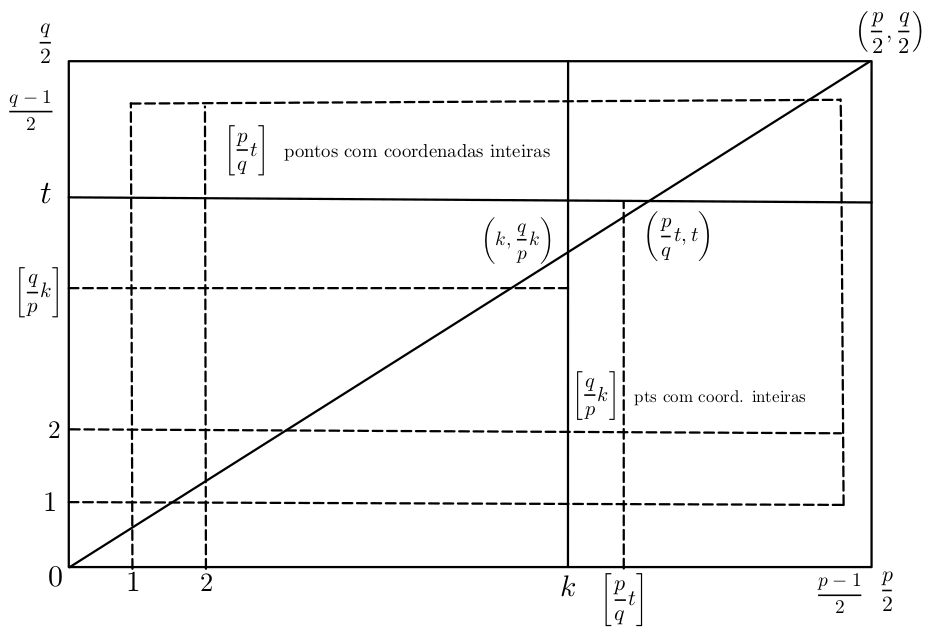
\includegraphics[width=\textwidth]{ImagemTN.png}
	\end{figure}
	A equação da reta por $(0,0), (p/2,q/2)$ é $y = x(q/p)$. Como $p/2,q/2\notin\mathbb{Z}$, os pontos interiores ao retângulo com coordenadas inteiras são aqueles no produto cartesiano
	\begin{align*}
	Z = \left\{ 1,2,\dots,\frac{p-1}{2} \right\}\times\left\{ 1,2,\dots,\frac{p-1}{2} \right\},
	\end{align*}
	de modo que 
	\begin{align*}
	|Z| = \frac{p-1}{2}\cdot\frac{q-1}{2}.
	\end{align*}
	Uma observação importante é que nenhum ponto de $Z$ está sobre a reta $y = x(q/p)$. Queremos contar a quantidade de pontos de $Z$ de uma maneira diferente e aplicar o Lema de Gauss II. 
	\par\vspace{0.3cm} Considerando a região entre a reta vertical $x_0 = k$ e abaixo da reta $y = x(q/p)$, sabemos que há $\displaystyle{ \left[ \frac{q}{p}\cdot k \right] }$ pontos com coordenadas inteiras. Logo, no interior de $\Delta{ABC}$ há
	\begin{align*}
	M_0 = \sum_{i=1}^{\frac{p-1}{2}}\left[ \frac{iq}{p} \right]
	\end{align*} 
	pontos com coordenadas inteiras. Analogamente, considerando a reta horizontal $y_0 = t$, vemos que há exatamente
	\begin{align*}
	M_1 = \sum_{i=1}^{\frac{q-1}{2}}\left[ \frac{ip}{q} \right]
	\end{align*}
	pontos com coordenadas inteiras no triângulo $\delta{ADC}$. Logo, 
	\begin{align*}
	M_0 + M_1 = |Z| = \frac{p-1}{2}\cdot\frac{q-1}{2}
	\end{align*}
	e, do Lema de Gauss II, segue que
	\begin{align*}
	\legendre[]{q}{p} = (-1)^{M_0}, \legendre[]{p}{q} = (-1)^{M_1},
	\end{align*}
	de modo que
	\begin{align*}
	\legendre[]{p}{q}\legendre[]{q}{p} = (-1)^{M_0+M_1} = (-1)^{\frac{p-1}{2}\cdot\frac{q-1}{2}}.
	\end{align*}
\end{proof}
\begin{lemma}
	\label{lema 92}
	Seja $p$ primo ímpar, $p\geq 5$. Então
	\begin{align*}
	\legendre[]{3}{37} = 1\Longleftrightarrow p\equiv \pm 1\bmod 12.
	\end{align*}
\end{lemma}
\begin{proof}
	Vamos dividir em casos.
	\begin{enumerate}[(i)]
		\item $p\equiv 1\bmod 3$
		Nesse caso, $\displaystyle{\legendre[]{p}{3} = 1}$. Pela LRQ,
		\begin{align*}
		\legendre[]{p}{3}\legendre[]{3}{p} = (-1)^{\frac{p-1}{2}} \Longrightarrow \legendre[]{3}{p} = (-1)^{\frac{p-1}{2}}.
		\end{align*}
		Logo, 
		\begin{align*}
		\legendre[]{3}{p} = 1 \Longleftrightarrow p\equiv 1\bmod 4 \Longrightarrow p\equiv 1\bmod 12\text{ pois } p\equiv 1\bmod 3.
		\end{align*}
		\item $p\equiv -1\bmod 3$
		Nesse caso, $\displaystyle{\legendre[]{p}{3} = -1}$. Pela LRQ,
		\begin{align*}
		\legendre[]{p}{3}\legendre[]{3}{p} = (-1)^{\frac{p-1}{2}} \Longrightarrow \legendre[]{3}{p} = -(-1)^{\frac{p-1}{2}}.
		\end{align*}
		Logo, 
		\begin{align*}
		\legendre[]{3}{p} = 1 \Longleftrightarrow p\equiv -1\bmod 4 \Longrightarrow p\equiv -1\bmod 12\text{ pois } p\equiv -1\bmod 3.
		\end{align*}
	\end{enumerate}
\end{proof}
\begin{example}
	A congruência $x^2\equiv 56\bmod 547$ tem solução?
\end{example}
\begin{solution}
	Temos que $547$ é primo e $56 = 2^3\cdot 7$, logo
	\begin{align*}
	\legendre[]{56}{547} = \legendre[]{2^3}{547}\legendre[]{7}{547} = \legendre[]{2}{547}\legendre[]{7}{547}.
	\end{align*}
	Como $547\not\equiv 1\bmod 8$, segue do Lema \eqref{lema 90} que $\displaystyle{\legendre[]{2}{547} = -1}$. Pela LRQ,
	\begin{align*}
	\legendre[]{7}{547}\legendre[]{547}{7} = (-1)^{273\cdot 3} = -1.
	\end{align*}
	Como $547\equiv 1\bmod 7$, então $\displaystyle{\legendre[]{547}{7} = 1}$, logo $\displaystyle{\legendre[]{7}{547} = -1}$ e $\displaystyle{\legendre[]{56}{547} = 1}.$ Logo, a congruência tem solução.
\end{solution}
\begin{example}
	A congruência $3x^2\equiv 466\bmod 467$ tem solução?
\end{example}
\begin{solution}
	Precisamos primeiro reescrever a congruência no formato $x^2\equiv b\bmod 467$ para aplicar a teoria. O primeiro passo é resolver $3z\equiv 1\bmod 467$, obtemos $z = 156$. Como $466\equiv -1\bmod 467$, então $3x^2\equiv 466\bmod 467$ é equivalente a $x^2\equiv -156\bmod 467$. Determinar se esta congruência tem solução é equivalente a determinar $\displaystyle{\legendre[]{-156}{467}}$. Note que $156 = 3\cdot 4\cdot 13$, logo
	\begin{align*}
	\legendre[]{-156}{467} = \legendre[]{-1}{467}\legendre[]{3}{467}\legendre[]{13}{467}, \text{ pois } 4 \text{ é quadrado.}
	\end{align*}
	Pelos Lemas \eqref{lema 85} e \eqref{lema 92}, $467\not\equiv 1\bmod 4$ e $467\equiv 1\bmod 12$, logo
	\begin{align*}
	\legendre[]{-156}{467} = -\legendre[]{13}{467}.
	\end{align*}
	Pela LRQ,
	\begin{align*}
	\legendre[]{13}{467}\legendre[]{467}{13} = (-1)^{6\cdot 233} = 1,
	\end{align*}
	ou seja,
	\begin{align*}
	\legendre[]{13}{467} = \legendre[]{467}{13}.
	\end{align*}
	Note que $467\equiv -1\bmod 13$ e $13\equiv 1\bmod 4$, logo
	\begin{align*}
	\legendre[]{467}{13} = \legendre[]{-1}{13} = 1.
	\end{align*}
	Daí, segue que
	\begin{align*}
	\legendre[]{-156}{467} = -\legendre[]{13}{467} = -1,
	\end{align*}
	e a congruência não tem solução.
\end{solution}


\end{document}